% =====================================================================
%  Data Mining  ·  SGH Warsaw School of Economics  ·  SMMD-ADA
%  Course script (skrypt): the lecture prose behind the slide decks.
%  Each block chapter follows its slide deck and adds what slides
%  cannot hold. Figures are shared with the decks (lecture_N/figures/).
%
%  Build:  pdflatex main.tex   (run twice for TOC/refs)
% =====================================================================
\documentclass[11pt,a4paper]{article}

% ---- encoding & fonts (pdflatex path) -------------------------------
\usepackage[T1]{fontenc}
\usepackage[utf8]{inputenc}
\IfFileExists{lmodern.sty}%
  {\usepackage{lmodern}\usepackage{microtype}}%
  {\usepackage[expansion=false]{microtype}}

% ---- layout ----------------------------------------------------------
\usepackage[a4paper,margin=2.6cm]{geometry}
\usepackage{amsmath,amssymb}
\usepackage{booktabs}
\usepackage{array}
\usepackage{multirow}
\usepackage{longtable}
\usepackage{enumitem}
\usepackage{graphicx}
\usepackage[hidelinks]{hyperref}

\newcommand{\yes}{\checkmark}
% Boxed aside for practical, from-the-trenches remarks.
\newenvironment{practice}
  {\par\medskip\noindent\begin{minipage}{\linewidth}
   \rule{\linewidth}{0.4pt}\par\smallskip
   \small\textbf{In practice.}\ }
  {\par\smallskip\rule{\linewidth}{0.4pt}\end{minipage}\medskip\par}

\title{\vspace{-1.5cm}\textbf{Data Mining}\\[0.3em]
\large Course script - a finance-first, problem-driven course\\[0.6em]
\normalsize SGH Warsaw School of Economics - SMMD-ADA}
\author{Daniel Wlazło}
\date{Autumn semester 2026 - Tuesdays 17:10--20:30 (4h blocks)}

\begin{document}
\maketitle
\thispagestyle{empty}

% =====================================================================
\section*{How to use this script}
\addcontentsline{toc}{section}{How to use this script}
This script is the written companion to the lecture slides: the same
argument, in full sentences, plus the details, caveats and worked numbers
that do not fit on a slide. Each block of the course has one chapter here,
one slide deck, and one lab notebook; the three are built from the same
dataset and tell one continuous story. Read the chapter after (or instead
of) the lecture; run the notebook alongside it.

\begin{center}\small
\begin{tabular}{@{}clll@{}}
\toprule
\# & Date & Topic & Lab notebook \\
\midrule
1 & 06.10 & Data mining \& CRISP-DM; EDA; \textbf{missingness}; features; project brief & \texttt{01} \\
2 & 13.10 & \textbf{Linear \& logistic regression}; regularisation; intro to evaluation & \texttt{02} \\
3 & 20.10 & Trees; SVM; \textbf{ensembles (RF, GBDT)}; honest evaluation; leakage & \texttt{03} \\
4 & 27.10 & Clustering (k-means, hierarchical, DBSCAN); PCA & \texttt{04} \\
5 & 03.11 & \textbf{Pattern discovery / Market Basket}; \textbf{text-mining basics} & \texttt{05} \\
6 & 10.11 & \textbf{Foundations of neural networks}; responsible ML & \texttt{06} \\
7 & 17.11 & Project defences (part I) + \textbf{Exam, term 0} (part II) & - \\
\bottomrule
\end{tabular}
\end{center}

Course organisation - learning outcomes, project rules and rubric, exam
format, datasets and tooling - is collected in Appendix~\ref{app:org}.

\tableofcontents
\newpage

% =====================================================================
% =====================================================================
\section{Block 1 - Data mining, EDA \& the anatomy of missing data}

\subsection{What data mining is - and is not}
Data mining is the craft of finding useful structure in data \emph{in order
to support a decision}, with methods that are honest about uncertainty. Every
part of that sentence carries weight. ``Useful'' rules out structure that is
statistically real but operationally irrelevant. ``Decision'' anchors the
whole exercise: someone will approve a loan, contact a customer, or set a
price differently because of what we find. And ``honest about uncertainty''
separates data mining from wishful thinking dressed in charts.

It is just as important to say what data mining is \emph{not}. It is not
running every algorithm in a library and keeping the one with the highest
accuracy - we will see in Block~3 how easily that procedure fools its
author. It is not ``the model said so'': a model output is an input to human
judgement, not a substitute for it. And it is not a replacement for
understanding the business problem; no amount of gradient boosting fixes a
mis-posed question. Throughout the course the direction is always the same:
we start from the decision and choose the method - never the reverse.

Where does the discipline sit on the map? Artificial intelligence is the
broadest ring: systems that behave ``intelligently'' by whatever mechanism.
Machine learning is the subset that learns from data rather than from
hand-written rules. Data mining is the part of machine learning (plus a good
deal of statistics and databases) aimed at extracting useful patterns from
business data. Statistics underpins all three rings - inference,
uncertainty quantification, experimental design. The borders are soft, and
industry job titles (``data scientist'') usually mean the union rather than
any single ring. Nothing in this course depends on the taxonomy; it exists
so that you can place what you learn here next to what you learn elsewhere.

\subsubsection{The promise - and where it fails in organisations}
Why do banks, telecoms and retailers fund this discipline at all? Because a
small \emph{relative} improvement applied to a large \emph{flow} of
decisions compounds into serious money. A toy calculation makes the logic
concrete (the numbers are invented, the structure is not). Suppose a lender
approves 100{,}000 loans a year at an average of 20{,}000 PLN, and credit
losses run at 3\% of the amount lent - 60 million PLN a year. A scoring
model that cuts those losses by 10\% \emph{relative}, at the same approval
rate, is worth 6 million PLN a year, every year, for the cost of a small
team and some computers. That is the promise: not one brilliant prediction,
but a slightly better decision repeated a hundred thousand times. The same
arithmetic explains why data mining lives most comfortably in businesses
with high decision volumes - lending, insurance pricing, marketing,
fraud - and least comfortably where decisions are few and each one is
idiosyncratic.

The same logic exposes where projects fail, and it is rarely in the
mathematics. The value of a data-mining project is a chain: data
$\rightarrow$ model $\rightarrow$ decision rule $\rightarrow$ execution -
and the weakest link caps the whole chain. In practice the chain breaks in
recognisable places. A model is built but nobody owns the decision it was
supposed to change, so it is admired and shelved. The predictions are
accurate but the business process cannot act on them - the collections
team has no capacity for the extra calls the model recommends. The model is
deployed but the input data pipeline differs subtly from the training
pipeline, so production scores drift away from notebook scores. Or - the
most common failure of all - the question was never a decision in the
first place: ``find something interesting in this data'' produces findings
that are interesting and change nothing. Industry surveys have reported for
years that a large majority of models never reach production; the reasons
above, not algorithmic weakness, dominate the post-mortems.

The lesson for this course is a habit of mind: before touching data, write
one sentence of the form ``because of this analysis, \emph{person X} will
do \emph{Y} differently''. If you cannot fill in the blanks, you do not yet
have a data-mining problem - you have data and curiosity, which is a fine
starting point but not a deliverable. Your course project is graded on
exactly this discipline: the framing marks are earned by the sentence
above, not by the model that follows it.

\subsection{A map of learning problems}
Before any method, a vocabulary. Machine-learning problems fall into three
broad paradigms:
\begin{description}[leftmargin=1.4em,style=nextline,itemsep=2pt]
  \item[Supervised learning.] The data come with \emph{labels} - for each
        historical case we know the outcome - and the goal is to predict the
        label for new cases. \emph{Will this applicant default?}
  \item[Unsupervised learning.] No labels; the goal is to find
        \emph{structure} in the data: groups of similar cases, co-occurrence
        patterns, compressed representations. \emph{Which customers are
        similar to each other?}
  \item[Reinforcement learning.] An agent takes actions, receives
        \emph{rewards}, and adapts its strategy. \emph{Which collections
        action should we try next?} We only mention this paradigm in the
        course, so that you can place it on the map.
\end{description}

Supervised learning itself comes in flavours, distinguished by the type of
target:
\begin{center}\small
\begin{tabular}{@{}lp{4.6cm}p{5.2cm}@{}}
\toprule
Task & Target & Credit example \\
\midrule
Binary classification & one of two classes & \texttt{default} $\in \{0,1\}$ \\
Multiclass classification & one of several classes & complaint category; rating grade \\
Regression & a continuous number & loss amount; recovery rate \\
Others (mentioned only) & ordinal, ranking, survival time & months until default \\
\bottomrule
\end{tabular}
\end{center}

The course concentrates on \textbf{binary classification} (the
probability-of-default thread of Blocks 2, 3 and 6) and \textbf{regression}
(Blocks 2--3); multiclass classification and the remaining task types appear in
passing where a method naturally generalises. The unsupervised paradigm gets
its own two blocks: clustering and dimensionality reduction (Block 4),
pattern discovery and text mining (Block 5).

Translating a business question into one of these tasks is the analyst's
job, and no algorithm does it for you. ``Will this applicant default?'' is
binary classification; ``how large will the loss be if they do?'' is
regression; ``which complaint team should read this email?'' is multiclass;
``do our customers form natural segments?'' is clustering; ``which products
are bought together?'' is association-rule mining. Getting this translation
wrong invalidates everything downstream, which is why it belongs to the
\emph{business understanding} phase, not to modelling.

Two subtleties hide inside the translation, and both will reappear later in
the course. First, \emph{the target itself is a design decision}, not a fact
of nature. ``Default'' sounds objective, but someone had to decide how many
days past due count as default, over what observation window, and measured
from which moment - and two teams with different definitions will build
models that cannot be compared. Whenever you receive a labelled dataset,
ask who defined the label, how, and whether that definition matches the
decision you are supporting. Second, the same business problem can often be
posed as more than one task: ``how risky is this applicant?'' can be binary
classification (default / no default), regression (expected loss), or
survival analysis (time until default). The cheapest formulation that
supports the decision wins; do not reach for the exotic one because it
sounds sophisticated. Retail credit overwhelmingly chooses binary
classification with a fixed outcome window precisely because the resulting
probability plugs directly into an approve/decline rule, a price, and a
capital calculation - the decision shapes the task.

\subsection{CRISP-DM: the spine of the course}
CRISP-DM (Cross-Industry Standard Process for Data Mining) structures every
project in this course: (1) business understanding, (2) data understanding,
(3) data preparation, (4) modelling, (5) evaluation, (6) deployment - drawn
as a loop, because deployment feeds back into business understanding. The
most important arrow in the diagram is the dashed one, from \emph{evaluation}
back to \emph{data understanding}: a disappointing evaluation is rarely fixed
by a fancier model; it is fixed by going back and understanding the data
better. Block~1 lives entirely in phases 1 and 2.

\begin{figure}[htbp]
\centering
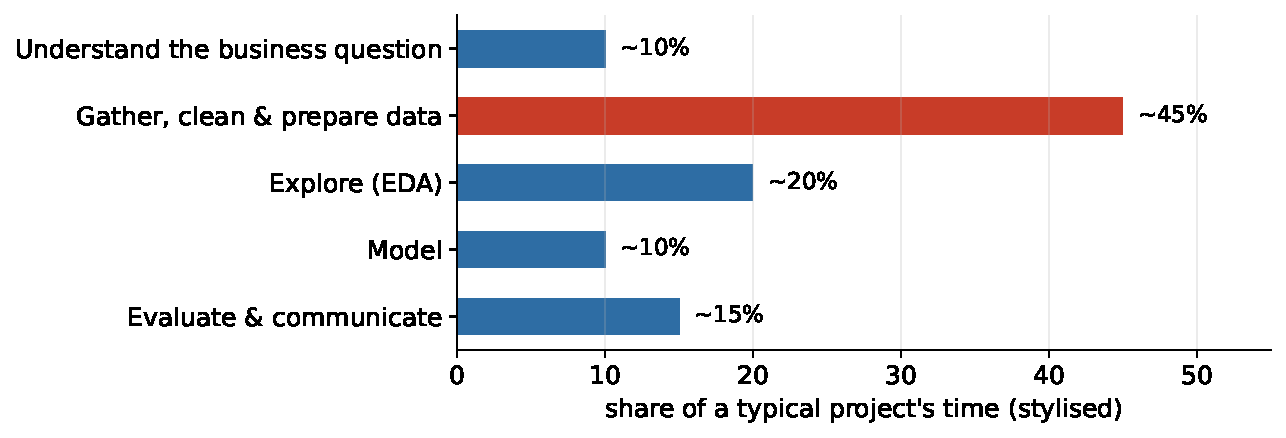
\includegraphics[width=0.62\textwidth]{lecture_1/figures/fig_time_split.pdf}
\caption{Where a typical project's time goes (stylised shares - surveys
differ, but data work always dominates). Modelling, the phase courses spend
most time on, is a small slice of real work.}
\label{fig:time}
\end{figure}

Figure~\ref{fig:time} explains why this course starts with data
understanding rather than algorithms: gathering, cleaning and exploring data
is where most of a project's calendar time - and most of its failure modes
- actually live.

\subsubsection{The six phases, seen from the trenches}
CRISP-DM reads like bureaucracy until you have watched a project die in
each phase. Here is what the boxes mean in practice, with the failure mode
each one exists to prevent.

\begin{description}[leftmargin=1.4em,style=nextline,itemsep=3pt]
  \item[1. Business understanding.] Turn a vague wish into a decision, a
        target, a unit of analysis, and success criteria \emph{in business
        terms}. The classic failure: a team spends months on ``predicting
        churn'' before anyone asks what the retention department would do
        with a churn score - and it turns out they have budget to contact
        two hundred customers a month, which changes the whole problem from
        ``predict churn'' to ``rank the two hundred most saveable
        customers''. One meeting in phase 1 would have replaced three
        months of phase 4.
  \item[2. Data understanding.] Collect the data, describe it, explore it,
        and audit its quality - the whole of this chapter. The failure it
        prevents is building on sand: documentation that lies (a field
        labelled ``monthly income'' that a legacy system has stored as
        annual income since a migration nobody remembers), keys that do not
        hold, missingness nobody counted. The cheapest place to discover a
        data problem is here; the most expensive is after deployment.
  \item[3. Data preparation.] Clean, join, transform, engineer features,
        and construct the modelling table. This is the phase that eats the
        calendar (Figure~\ref{fig:time}) and the phase where leakage traps
        are laid: joins that quietly use future information, transforms
        fitted on all rows, duplicates manufactured by a many-to-many merge.
        Every preparation step is a modelling decision wearing overalls.
  \item[4. Modelling.] Choose model families, fit, tune. Genuinely the
        easiest phase - a few library calls - which is exactly why
        beginners overweight it. The discipline: start with the simplest
        baseline that could work, so that every added complexity can be
        judged against it (Block~2 makes this concrete).
  \item[5. Evaluation.] Not ``compute the accuracy'' but: does the model,
        evaluated honestly, support the decision from phase 1 well enough
        to act on? This is where you discover that the brilliant score was
        leakage, that the model fails on exactly the segment the business
        cares about, or that the data does not contain the signal you hoped
        for. Hence the dashed arrow: evaluation routinely sends you back to
        phase 2, and a project plan with no room for that loop is a
        fiction.
  \item[6. Deployment.] The model leaves the notebook: scoring pipelines,
        monitoring, documentation, handover. Failure mode one: the feature
        code is re-implemented for production and computes something
        subtly different, so the deployed model is not the validated one.
        Failure mode two: nobody monitors, the world drifts, and the model
        degrades silently for a year. Deployment is where data mining
        stops being a study and starts being a liability - which is why
        regulated industries audit it.
\end{description}

Two remarks on using the framework well. First, the phases are a checklist
of \emph{questions}, not a waterfall of gates: real projects run several
loops, each deeper than the last, and a first pass through all six phases
in a week (a ``walking skeleton'' of the project) beats six weeks spent
perfecting phase 3. Second, the phase boundaries are where
misunderstandings hide, because responsibility changes hands - the
business owner frames, the analyst prepares and models, engineering
deploys. Write down what was agreed at each boundary; the written form is
the cheap insurance. Your course project is a miniature of exactly this
cycle, and its rubric mirrors the phases - framing, preparation,
modelling, evaluation, interpretation - so the process is not just
background theory; it is the marking scheme.

\subsection{The business problem for the whole term}
We are a retail lender. At application time we observe a customer's
characteristics; we must decide whether to grant credit. The modelling
question: given what we know \emph{at application time}, how likely is the
customer to default - and what should we do about it?

One row of our table is one customer with one loan application. This choice
of the \emph{unit of analysis} deserves a moment, because it is the first
decision nobody teaches. The unit fixes what a prediction means and when it
can be used. A customer with three loans could be three rows or one; your
metrics change either way. Mixing units - some rows customers, some
applications - silently double-counts people. Whenever you meet a new
table, ask what a row is before you ask anything else.

\subsubsection{The unit of analysis: a second worked example}
The application-level table is not the only way to slice a lending
portfolio, and seeing a second slicing makes the concept stick. Consider a
\emph{customer-month} panel: one row per customer per calendar month on the
books, with behavioural fields (balance, payments made, days past due) and
a target such as ``defaults within the next 12 months''. Banks use exactly
this shape for \emph{behavioural} scoring of existing customers, next to
the \emph{application} scoring we build in this course.

A toy portfolio shows how much the unit changes the numbers. Ten customers
are observed for twelve months each - 120 customer-month rows - and two
of the customers default once during the year. At the customer level the
default rate is $2/10 = 20\%$. At the customer-month level it is
$2/120 \approx 1.7\%$. Same portfolio, same events, a twelvefold difference in
the headline rate - and neither number is wrong; they answer different
questions (``will this customer ever default this year?'' versus ``will
this customer default in a given month?''). Every downstream choice moves
with the unit: the features (application data versus recent behaviour),
the moment the prediction is usable (once, at application, versus every
month), and the class balance the model faces.

The panel shape also plants a landmine we will defuse properly in Block~3:
the twelve rows of one customer are not twelve independent observations.
They share the same person, the same habits, the same eventual outcome. A
random row-level train/test split puts months 1--6 of a customer in
training and months 7--12 in test - the model has effectively seen the
test customers already, and every score is inflated. The split must be by
\emph{customer} (or by time), not by row. The general rule: whatever your
unit of analysis, ask what the true independent unit is, and split on
that. For our application-level table the two coincide, which is one
reason it is the right training ground.

The Block~1 portfolio has 4{,}000 customers and 18 columns; the primer and
Block~1 lab load it via \texttt{finance\_data.load\_credit()}, which fetches
the classic German Credit data from OpenML or generates a synthetic Polish
portfolio with the same interface (the labs pin the synthetic source for
reproducibility; from Block~2 onward the modelling labs switch to the real
Taiwan portfolio via \texttt{load\_taiwan()}). Alongside ordinary application fields - age, income,
housing, loan purpose, existing loans, savings - it contains three columns
placed there deliberately: \texttt{months\_since\_last\_delinquency}, which
is \emph{structurally missing} for customers who were never delinquent;
\texttt{monthly\_income\_pln} with income-dependent missingness; and
\texttt{collections\_contact}, a leakage trap we defuse in
Section~\ref{sec:leakage} and detonate, on purpose, in Block~3.

\subsubsection{The data you will never see: selection bias}
One question should precede even the first histogram: \emph{how did rows get
into this table?} A lender's portfolio contains only \emph{approved} loans.
Rejected applicants have no default outcome - they are simply absent -
so any model trained here learns the behaviour of the survivors of
yesterday's approval policy. For applicants unlike anyone previously
approved, the model extrapolates, and its confidence in that region is
borrowed, not earned. Credit scoring is unusual in having a name and a
toolbox for the problem (\emph{reject inference}: inferring what the
rejected would have done); most other domains quietly ignore the same
pattern - churn models see only customers who were acquired, hiring models
see only people who were hired. Two things matter on day one: selection
bias cannot be fixed by collecting more data \emph{from the same source},
and every dataset deserves the how-did-rows-get-here question before any
conclusion leaves the room.

\paragraph{Why the approved-only sample distorts what a model learns.}
It is worth seeing the mechanics, because ``the sample is biased'' sounds
abstract until you watch it bend a relationship. Toy numbers, chosen for
arithmetic rather than realism. In the full applicant population there are
two groups: low-utilisation applicants who default at 10\%, and
high-utilisation applicants who default at 50\% - a strong, honest risk
signal. Yesterday's policy approved essentially all of the low group but
only a carefully chosen tenth of the high group: the ones with high
incomes and long employment, who default at 20\% rather than 50\%. Now
look at the training table this policy left behind. Within it, moving from
low to high utilisation raises the observed default rate from 10\% to 20\%
- the model learns a modest slope, when the true population slope runs
from 10\% to 50\%. The signal is \emph{attenuated}, because the policy
systematically removed the worst cases from exactly the region where the
feature mattered most. Worse, the model has never seen an \emph{ordinary}
high-utilisation applicant at all, so when tomorrow's policy asks it to
score one, it confidently applies the 20\% pattern learned from an elite
subgroup. The general phenomenon: past selection on (or correlated with)
your features flattens, bends, or even reverses the relationships a model
estimates, and it does so invisibly - the training data contains no trace
of the people who were filtered out.

\paragraph{What reject inference tries to do.} Since the problem cannot be
ignored in credit scoring - the score will be applied to the full
applicant population, not the approved one - the industry has developed
partial remedies, worth knowing by name even though their details are
beyond this course. The cleanest is \emph{outcome data from elsewhere}:
credit-bureau records sometimes show how a rejected applicant performed on
a loan granted by a competitor, turning some rejects into labelled rows.
The statistical family includes \emph{reweighting} (make the approved
sample resemble the applicant population on observables) and
\emph{extrapolation or parcelling} (score the rejects with an interim
model and assign them inferred outcomes, in proportion to their estimated
risk). The honest caveat applies to all of them: they infer the rejects'
outcomes from a model trained on the approved - the very extrapolation we
distrust - so they encode assumptions rather than replace missing facts.
The gold standard is experimental: approve a small random slice of
applicants who would normally be rejected, and observe what actually
happens. It is the only approach that produces real labels from the
unseen region, and it costs real money in defaults - a controlled price
paid for knowledge, which risk departments weigh explicitly. If one idea
survives from this subsection, let it be this: the absence of data is
itself data about the process that produced your table, and no amount of
modelling sophistication can conjure the missing region back.

\subsection{Exploratory data analysis}
\label{sec:eda}
EDA is not a ritual to perform before the ``real work''. It \emph{is} real
work: most projects fail quietly here, not loudly in modelling. The
checklist: shape and types; target balance; univariate distributions;
bivariate relationships with the target; data quality (duplicates, outliers,
missingness).

\subsubsection{First contact}
Four commands before anything else: \texttt{df.shape} (how much data?),
\texttt{df.dtypes} (what does pandas think each column is?),
\texttt{df.head(10)} (do the values look like the documentation promised?),
and \texttt{df.describe(include="all")} (ranges, counts, uniques). You are
looking for numbers stored as strings (\texttt{"12 000"}, \texttt{"N/A"}),
categorical levels that differ only by case or spelling, minima and maxima
that make no physical sense, and \texttt{describe()} counts smaller than
\texttt{len(df)} - the first sign of missingness.

\paragraph{Reading \texttt{describe()} like a practitioner.} The output of
\texttt{describe()} is a dense little report, and experienced analysts read
it in a fixed order, each row answering a specific question. \texttt{count}
against \texttt{len(df)}: any shortfall is missingness - note the column
and the size of the gap before doing anything else. \texttt{mean} against
the \texttt{50\%} row (the median): a mean well above the median announces
right skew (income, balances, anything monetary); well below, left skew.
\texttt{std} against the mean: a standard deviation of the same order as
the mean, on a positive variable, is another skew fingerprint - a
symmetric variable that ``wanted'' to go negative but cannot. \texttt{min}:
should this variable ever be zero or negative? A negative income or a
zero age is a data-entry question, and a large pile of exact zeros may be
a hidden category (``no savings account'') rather than a measured amount.
\texttt{max}: is it physically plausible, and is it suspiciously round?
A maximum of exactly 999{,}999 is a sentinel wearing a number's clothing.
For categorical columns, \texttt{unique}, \texttt{top} and \texttt{freq}
carry the same kind of signal: \texttt{unique} close to \texttt{len(df)}
means the column is an identifier in disguise (and identifiers are never
features); \texttt{freq} close to \texttt{len(df)} means the column is
nearly frozen and likely carries no information; a \texttt{unique} count
higher than the documentation promises means phantom levels - typos, case
variants, or trailing spaces. Ten seconds per column, and you have a
working map of where the problems live. The point is not the tool - any
summary table works - but the habit of interrogating each number instead
of scrolling past it.

Then verify the key: does \texttt{customer\_id} really identify rows
uniquely? Duplicated rows are double-counted evidence, and a duplicate that
lands in both training and test data inflates every score you will ever
compute on it - a cousin of the leakage problem of Block~3. In our
portfolio the key holds and there are no full-row duplicates; in the wild,
repeated exports glued together and joins that multiplied rows are everyday
occurrences.

Know your variable types, because the type decides the plot, the summary
statistic, and (later) the encoding: numeric continuous (income, DTI),
numeric discrete (number of existing loans - often better treated as
categories), categorical nominal (purpose, region), categorical ordinal
(checking status: none $<$ low $<$ medium $<$ high - the order matters,
keep it), dates and times (time zones bite, and date columns enable
leakage), free text (its own pipeline, Block 5), and identifiers -
\emph{never} features.

Behind this practical typology sits the classical theory of
\emph{measurement scales} (Stevens, 1946), worth knowing because it says
which operations are meaningful at all:

\begin{center}\small
\begin{tabular}{@{}lllp{3.6cm}@{}}
\toprule
Scale & Defining property & Meaningful operations & Example \\
\midrule
Nominal & categories, no order & $=$, $\neq$ & purpose, region \\
Ordinal & ordered, unknown gaps & $<$, $>$ & checking status, ratings \\
Interval & equal gaps, no true zero & $+$, $-$ & temperature in °C; calendar dates \\
Ratio & true zero exists & $\times$, $\div$ & income, loan amount, age \\
\bottomrule
\end{tabular}
\end{center}

The scale limits the statistics: a mean of nominal codes is nonsense, a
median needs at least an ordinal scale, and ``twice as much'' requires a
true zero - 40°C is not twice as warm as 20°C, but a 40{,}000 PLN loan is
exactly twice a 20{,}000 one. The scale also constrains encodings, which
matters from Block 2 onward: coding a nominal variable as integers invents
an order that is not there, while one-hot-encoding an ordinal variable
throws a real order away.

\paragraph{Stevens' scales, seen through transformations.} There is an
elegant way to remember what each scale licenses: ask which
\emph{relabellings} of the data would leave its meaning intact. A nominal
variable survives any one-to-one renaming - call the purposes A, B, C or
1, 7, 42, nothing changes - so only statements invariant to renaming
(equality, counts, the mode) are meaningful. An ordinal variable survives
any order-preserving transformation - recode none/low/medium/high as
0/1/2/3 or as 0/10/11/99 and the order still holds - so medians and
quantiles are safe (they depend only on order), but means are not: the two
recodings above give different means for the same data. An interval
variable survives shifts and rescalings ($x \mapsto ax+b$): Celsius and
Fahrenheit disagree about every number yet agree about every
\emph{difference} of temperatures, which is why differences are meaningful
and ratios are not. A ratio variable survives only rescaling
($x \mapsto ax$): PLN and EUR disagree about the numbers but agree that one
loan is twice another. A statistic is meaningful on a scale exactly when
it is invariant under that scale's permissible transformations - a
one-line rule that settles most ``can I average this?'' arguments. One
practical footnote: applied work bends these rules constantly (survey
research averages ordinal rating scales as a matter of routine), and the
bending is often harmless. The theory is not a police force; it is a
warning system that tells you \emph{when} a summary depends on an
arbitrary coding choice - and therefore when a critic can legitimately
attack your number.

\subsubsection{The target comes first}
\begin{figure}[htbp]
\centering
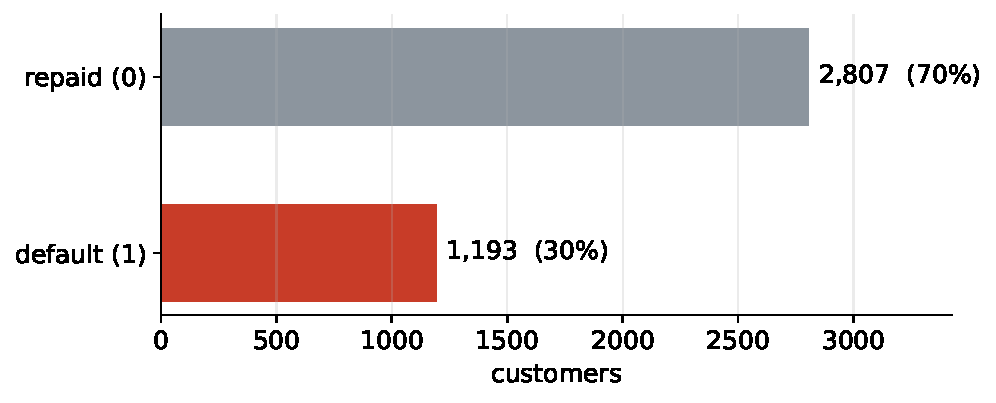
\includegraphics[width=0.66\textwidth]{lecture_1/figures/fig_target_balance.pdf}
\caption{Target balance in the course portfolio.}
\label{fig:balance}
\end{figure}

About 30\% of the portfolio defaults (Figure~\ref{fig:balance}). A model
that always predicts ``repaid'' is therefore right seven times out of ten
- and completely useless, because it approves everyone. This is the
\emph{accuracy trap}: on imbalanced problems, accuracy rewards ignoring the
minority class. Real PD portfolios are far more extreme (1--5\% default
rates), which makes the trap deeper. The honest metrics for imbalanced
classification are the subject of Block~3; for now, note the imbalance and
distrust accuracy.

Why check the target first, before any feature? Three reasons. The base
rate is your \emph{baseline}: every model you ever build must beat the
trivial strategy of predicting the majority class, and you cannot know
what that strategy scores until you know the balance. The base rate also
calibrates your reading of every bivariate plot to come - a segment
defaulting at 39\% is alarming against a 30\% portfolio and unremarkable
against a 38\% one. And the imbalance previews an economic asymmetry that
will drive Block~3: the two errors do not cost the same. Approving a
future defaulter loses (part of) the principal; declining a good customer
loses only the margin. When one error is many times dearer than the other,
a metric that weights them equally - accuracy - is answering a question
nobody asked. The target distribution is one number, and it silently
parameterises the entire project.

\subsubsection{Univariate structure}
\begin{figure}[htbp]
\centering
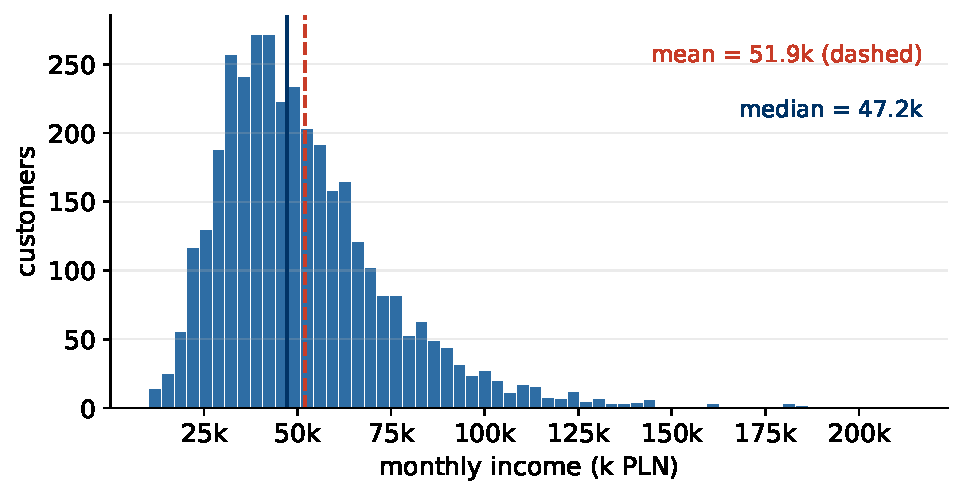
\includegraphics[width=0.72\textwidth]{lecture_1/figures/fig_income_hist.pdf}
\caption{Monthly income: right-skewed, mean above median.}
\label{fig:income}
\end{figure}

Income (Figure~\ref{fig:income}) is right-skewed: a minority of high earners
pulls the mean above the median. Skew is information. It tells you which
summary to report (the median, for skewed variables), and it hints that a
transform may help. Figure~\ref{fig:log} shows the same variable through a
log lens: nearly symmetric. Monetary amounts - income, savings, losses -
almost always deserve a log look, because money behaves multiplicatively: the
difference between 3 and 6 thousand PLN is a doubling, like the difference
between 30 and 60 thousand, not like the difference between 30 and 33.

\begin{figure}[htbp]
\centering
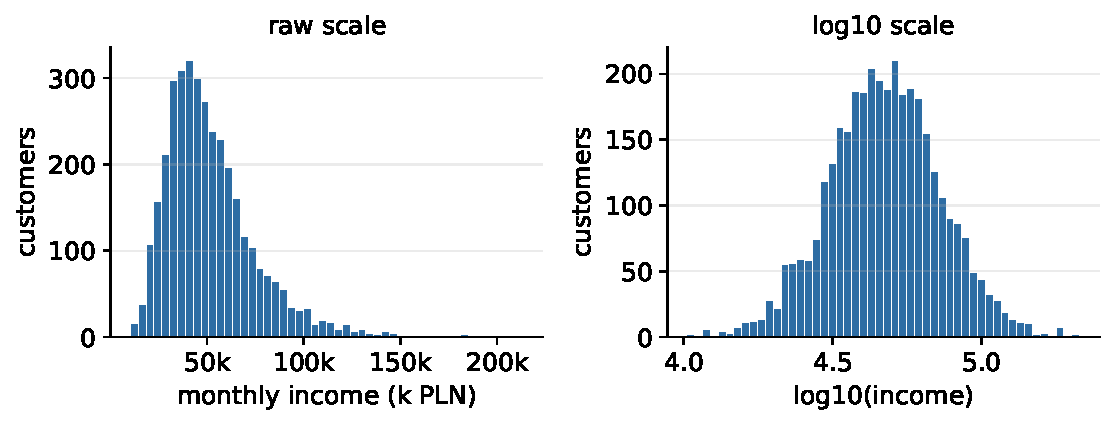
\includegraphics[width=0.8\textwidth]{lecture_1/figures/fig_income_log.pdf}
\caption{The same income variable, raw and log scale.}
\label{fig:log}
\end{figure}

\paragraph{Why the log lens works.} The pattern is too reliable to be a
coincidence, and it is not one. Quantities that grow by \emph{proportional}
steps - salaries raised by percentages, wealth compounding at rates,
firms growing relative to their size - are products of many multiplicative
factors: after $n$ periods, $x_n = x_0 \cdot g_1 \cdot g_2 \cdots g_n$.
Take logarithms and the product becomes a sum,
$\log x_n = \log x_0 + \sum_i \log g_i$, and sums of many small
independent contributions are exactly what the central limit theorem
domesticates: approximately normal. So a multiplicatively generated
variable is approximately \emph{log}normal - symmetric on the log scale,
right-skewed with a long tail in raw units. This is why the log transform
is not a cosmetic trick that happens to prettify histograms: it is the
change of coordinates in which the process that generated the data is
additive, and in which ``equal distances'' mean ``equal ratios'' - the
comparison that actually matters for money. Three practical footnotes.
Use $\log(1+x)$ (\texttt{np.log1p}) when the variable contains legitimate
zeros - a zero savings balance is information, not an error, and plain
$\log$ would discard the row. Never log a variable with genuine negative
values (profits, balance changes); other transforms exist for those.
And remember the lens metaphor cuts both ways: after modelling on the log
scale, effects are multiplicative in the original units - ``+0.1 in log
income'' means ``about 10\% more income'', a reading you must translate
back for any human audience.

Alongside the shapes, run sanity checks for implausible values: ages outside
$[18, 100]$; negative incomes; sentinel codes (a suspicious spike at
999{,}999 usually means ``missing'' coded as a number); unit mixes (monthly
versus annual salary, PLN versus EUR); too-round values (everyone earning
exactly 5{,}000 suggests a form default); and frozen columns with one value
everywhere (a broken export). Each red flag is a \emph{question for the data
owner}, not a value to silently ``fix''. The checks cost three lines of
pandas and have saved careers.

\paragraph{Sanity checks are hypotheses, not chores.} There is a mindset
shift hidden in the list above. A weak analyst runs generic checks and
scrolls the output; a strong one writes down, \emph{before looking}, what
the data must satisfy if it is what it claims to be - and then tests each
statement like a hypothesis. ``Every age lies in $[18,100]$, because the
bank does not lend to minors.'' ``No application date precedes the
product's launch.'' ``Instalment never exceeds the loan amount.''
``\texttt{debt\_to\_income} equals total debt divided by income, to
rounding error'' - derived columns can be recomputed and compared, and a
mismatch means either the documentation or the pipeline is wrong. Each
check has only two outcomes, and both are valuable: it passes, and one
corner of the data is certified; or it fails, and you have found - for
the cost of one line of code - either a data defect or a hole in your own
understanding of the business. The second discovery is the more valuable
one. Checks that pass also earn their keep later: rerun on every data
refresh, they become a tripwire that catches upstream changes before the
model does.

For categorical variables, inspect the levels. Typos and case variants
create phantom categories. Rare levels (below 1--2\% of rows) often get
grouped into \texttt{other} before modelling - but only after checking
that they are not special: a tiny segment can carry a very high default
rate, and grouping it away destroys exactly the signal a lender cares about.

\subsubsection{Bivariate structure: what moves with the target}
The quickest model-free signal check is the binned default-rate plot: cut a
numeric feature into quantile bins and plot the default rate per bin.
Figure~\ref{fig:util} shows the result for credit utilisation - monotone
and steep, the signature of a strong candidate feature, and exactly what
credit-risk domain knowledge predicts.

\begin{figure}[htbp]
\centering
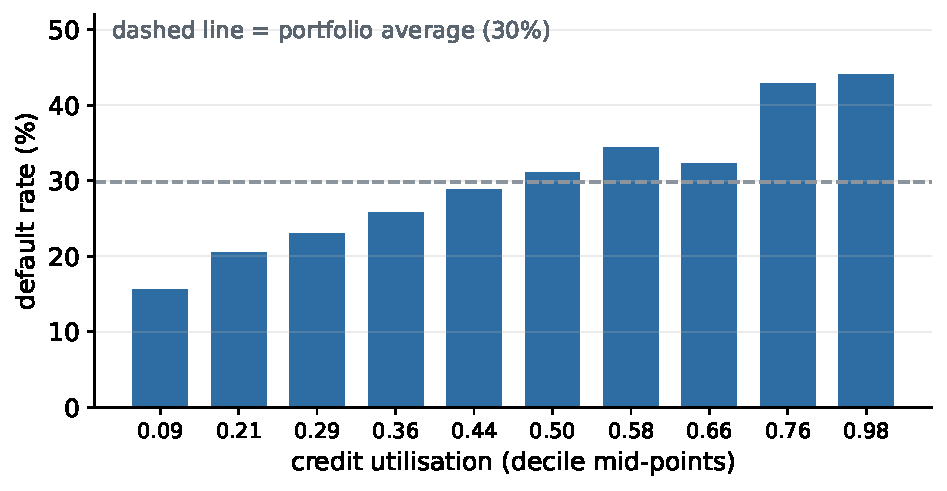
\includegraphics[width=0.72\textwidth]{lecture_1/figures/fig_default_by_utilization.pdf}
\caption{Default rate by credit-utilisation decile.}
\label{fig:util}
\end{figure}

\begin{figure}[htbp]
\centering
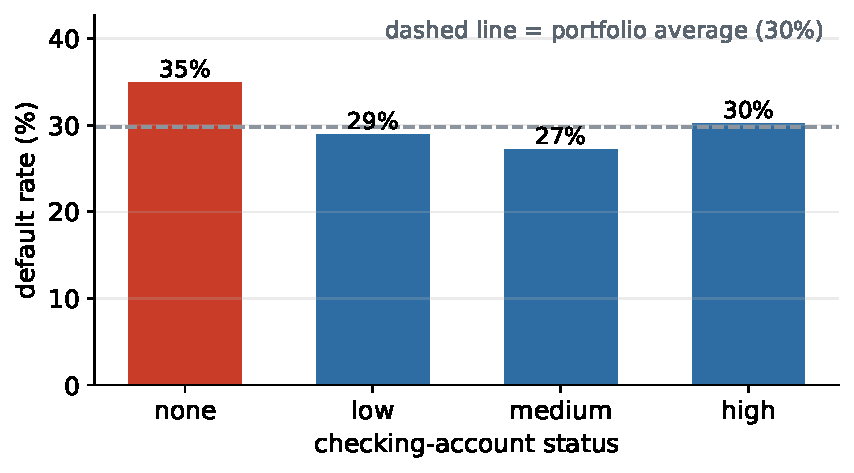
\includegraphics[width=0.6\textwidth]{lecture_1/figures/fig_default_by_checking.pdf}
\caption{Default rate by checking-account status.}
\label{fig:checking}
\end{figure}

For categorical features, compare each level's default rate with the
portfolio average (Figure~\ref{fig:checking}). ``No checking account'' is
the riskiest level - the bank cannot see those customers' cash flows, an
effect so robust that it survives from the 1990s German Credit data to
today's portfolios. Two cautions. First, mind the group sizes: a default
rate computed on thirty customers is noise, and eyeballing differences of a
few percentage points between small groups is how false ``insights'' are
born. Second, these are raw associations, not effects: the ``none'' group
differs from the ``high'' group in many other ways at once.

\paragraph{How noisy is a rate on $n$ customers?} The first caution
deserves numbers, because ``small groups are noisy'' becomes usable only
when you can say \emph{how} noisy. A default rate estimated on $n$
customers with true rate $p$ has standard error
$\sqrt{p(1-p)/n}$. Plug in toy values near our portfolio's balance:
with $p = 0.3$ and $n = 30$, the standard error is
$\sqrt{0.3 \cdot 0.7 / 30} \approx 0.084$ - more than eight percentage
points. Two thirty-customer groups drawn from the \emph{same} population
will routinely show rates like 27\% versus 37\%, a gap that looks like an
insight and is pure sampling noise. Grow the group to $n = 300$ and the
standard error falls to about 2.6 points; at $n = 3{,}000$, to under one
point. A serviceable habit: annotate every grouped-rate plot with the
group sizes (or error bars), and refuse to interpret any difference
smaller than a couple of standard errors. This is also why the interaction
segment of Section~\ref{sec:fe} quotes its $n$ alongside its rate - a
rate without its denominator is an anecdote wearing a percentage sign.

\subsubsection{Correlations - a first map, handled with care}
\begin{figure}[htbp]
\centering
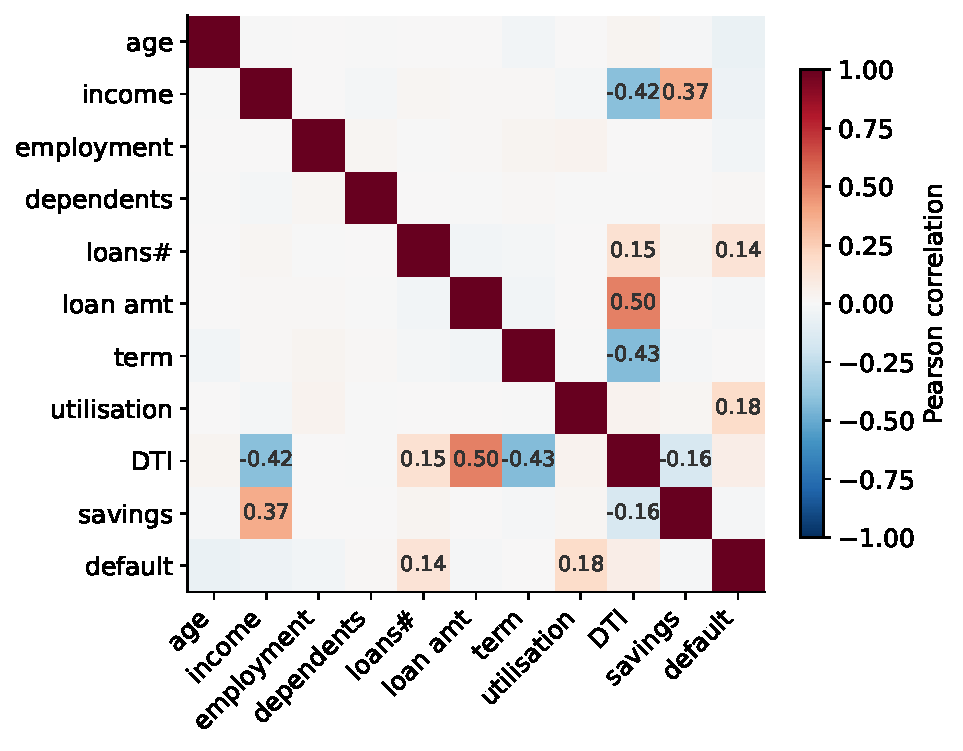
\includegraphics[width=0.6\textwidth]{lecture_1/figures/fig_corr_heatmap.pdf}
\caption{Pearson correlations among numeric features and the target
(only $|r| \geq 0.25$ annotated).}
\label{fig:corr}
\end{figure}

The correlation matrix (Figure~\ref{fig:corr}) gives one picture of which
features move together and which move with the target. In our portfolio,
credit utilisation ($r \approx 0.18$) and the number of existing loans
($r \approx 0.14$) stand out for \texttt{default} - current debt load
beats income - and income correlates visibly with savings, as the domain
would predict. Strongly correlated feature pairs ($|r| > 0.8$) are
candidates for dropping one member; nearly-duplicate features add
instability without adding information.

Four caveats keep the tool honest. Correlation is not causation - ice
cream sales correlate with drownings because summer causes both. Pearson's
$r$ sees only straight lines - a perfect U-shaped relationship can score
$r \approx 0$. A single extreme point can manufacture correlation where none
exists. And when variables are heavily skewed, Spearman's rank correlation
- which only asks ``do they move in the same direction?'' - is the more
robust lens. A correlation matrix generates \emph{hypotheses}, never
conclusions.

\paragraph{Correlation, formally.} Pearson's product-moment correlation
between variables $x$ and $y$ over $n$ observations is
\[
r_{xy} \;=\; \frac{\sum_{i=1}^{n}(x_i-\bar{x})(y_i-\bar{y})}
{\sqrt{\sum_{i=1}^{n}(x_i-\bar{x})^2}\,\sqrt{\sum_{i=1}^{n}(y_i-\bar{y})^2}}
\;=\; \frac{\operatorname{cov}(x,y)}{s_x\, s_y},
\]
a number in $[-1,1]$ measuring the strength of the \emph{linear}
relationship; it is invariant to shifting and (positive) rescaling of either
variable, which is why units do not matter. \emph{Spearman's} $\rho$ is
simply Pearson's $r$ computed on the \emph{ranks} of the data; with no ties
it reduces to
\[
\rho \;=\; 1 - \frac{6\sum_{i=1}^{n} d_i^{2}}{n(n^{2}-1)},
\qquad d_i = \operatorname{rank}(x_i) - \operatorname{rank}(y_i),
\]
and measures \emph{monotone} association: it is immune to any monotone
transform (log included) and far more robust to outliers. \emph{Kendall's}
$\tau$ counts concordant versus discordant pairs,
$\tau = (n_c - n_d)/\binom{n}{2}$; it has a clean probabilistic reading
(``how much more likely are two random customers to be ordered the same way
on both variables?'') and is preferred for small samples with many ties,
at $O(n \log n)$ cost against $O(n)$ once ranks are sorted.

Two practical remarks complete the picture. First, a Pearson correlation
against a \emph{binary} target (our \texttt{default}) is the
\emph{point-biserial} correlation. Its magnitude is mechanically bounded
well below 1 when the classes are imbalanced, so small-looking numbers can
accompany strong signals: utilisation's modest $r \approx 0.18$ coexists
with the steep decile gradient of Figure~\ref{fig:util} - from 15\% to
44\% default. Judge features against a 0/1 target by grouped rates and
(later) by model-based measures, not by $r$ alone. Second, Pearson and
Spearman apply to numeric (at least ordinal, for Spearman) variables; for a
pair of \emph{nominal} variables the analogous tool is Cramér's $V$, built
from the $\chi^2$ statistic of the contingency table,
$V=\sqrt{\chi^{2}/\bigl(n\cdot(\min(k,l)-1)\bigr)}$ for a $k \times l$
table, ranging from 0 (independence) to 1.

\paragraph{The ecological fallacy.} One more caveat belongs on the list,
because aggregated data invites it constantly: a correlation computed
across \emph{groups} says nothing reliable about individuals within them.
Suppose you correlate, across the regions of a country, average income
with regional default rate, and find that richer regions default less. It
does not follow that richer \emph{individuals} default less - the
individual-level relationship could be weaker, absent, or even reversed,
because regions differ in a hundred other ways (industry mix, product mix,
the lender's regional policies) that are averaged into the group figures.
The classic demonstrations in the statistics literature show group-level
and individual-level correlations differing not just in size but in sign.
The trap matters in practice because aggregated data is so often the only
data available - published statistics, market research, competitor
benchmarks all come pre-averaged. The discipline: state explicitly at
which level a correlation was computed, and refuse to let a group-level
number masquerade as a statement about persons. It is the mirror image of
Simpson's paradox below - both are failures of moving between levels of
aggregation without paying the toll.

\paragraph{Simpson's paradox.} One more way a bivariate summary can lie:
the aggregate trend can point the opposite way from the trend inside every
subgroup. Figure~\ref{fig:simpson} shows a constructed credit example -
in aggregate, bigger loans look \emph{safer}, because high-income customers
take the big loans; within each income band, bigger loans are riskier. Both
statements are true; only the within-band one is useful for a lending
decision. Before concluding from any bivariate plot, ask: \emph{compared
within what?} Segment first, conclude second.

The paradox stops feeling like magic once you do the arithmetic yourself,
so here is a toy portfolio (invented numbers, engineered to be transparent)
with two income bands and two loan sizes:

\begin{center}\small
\begin{tabular}{@{}llrrr@{}}
\toprule
Income band & Loan size & Loans & Defaults & Default rate \\
\midrule
Low income  & small & 200 & 40 & 20\% \\
Low income  & big   &  50 & 15 & 30\% \\
High income & small &  50 &  4 &  8\% \\
High income & big   & 200 & 24 & 12\% \\
\bottomrule
\end{tabular}
\end{center}

Within the low-income band, big loans are riskier (30\% versus 20\%);
within the high-income band, big loans are riskier again (12\% versus
8\%). Now pool the bands. Small loans: $200+50=250$ loans with $40+4=44$
defaults - a rate of $44/250 = 17.6\%$. Big loans: $50+200=250$ loans
with $15+24=39$ defaults - a rate of $39/250 = 15.6\%$. In aggregate,
big loans look \emph{safer}, even though they are riskier inside every
single band. The engine of the reversal is the lopsided mix: 80\% of big
loans sit in the low-risk high-income band, while 80\% of small loans sit
in the high-risk low-income band, so the pooled comparison is mostly
comparing income bands, not loan sizes. Income here is a
\emph{confounder} - a variable associated with both the feature and the
outcome - and pooling lets it impersonate the feature. The practical
defences: segment by the suspected confounder before concluding (as the
within-band rows do); and be suspicious whenever a pooled comparison
contradicts domain sense, because an unbalanced mix is usually hiding
underneath. Note finally what the paradox does \emph{not} say: neither
level of aggregation is automatically the truth. Which comparison is
right depends on the causal question being asked - for ``should loan
size worry me for a given applicant?'', the within-band answer is the
relevant one, because the applicant's income is known at decision time.

\begin{figure}[htbp]
\centering
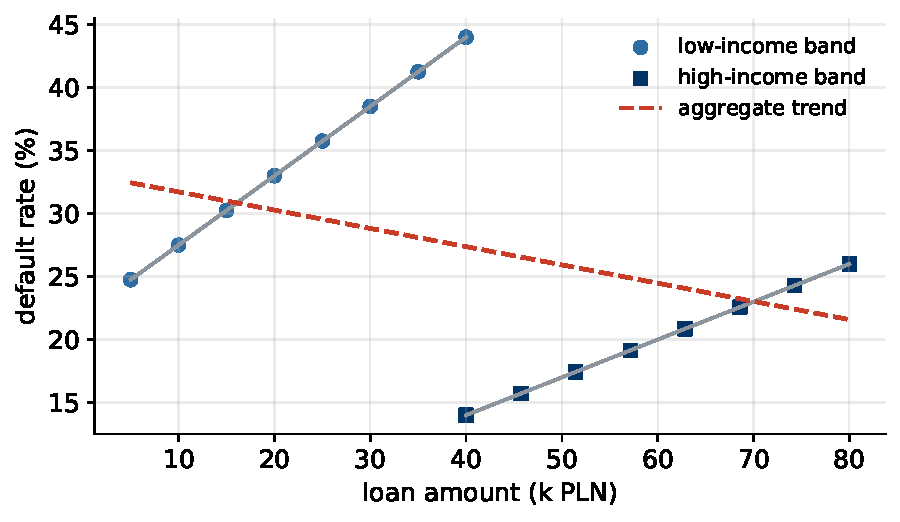
\includegraphics[width=0.56\textwidth]{lecture_1/figures/fig_simpson.pdf}
\caption{Simpson's paradox (illustrative data): the aggregate slope (dashed)
reverses the within-group slopes.}
\label{fig:simpson}
\end{figure}

The definitive argument for plotting rather than trusting summaries is
Anscombe's quartet (Figure~\ref{fig:anscombe}): four datasets with the same
means, variances, correlation ($r = 0.816$) and regression line - and four
completely different stories, including one where the ``relationship'' is a
single outlier. Summary statistics hide; plots reveal.

Anscombe built the quartet by hand in 1973 to attack a then-common
attitude he quoted as ``numerical calculations are exact, but graphs are
rough'' - and his deeper point survives every improvement in tooling
since. A summary statistic is a lossy compression of the data, chosen in
advance; it can only answer the question it was designed for, and it is
silent about everything else. The four panels are precisely the failure
modes an analyst meets in the wild: a genuinely linear relationship (the
one case where the summaries tell the truth); a smooth \emph{curve}, for
which a correlation is the wrong question; a clean line plus one outlier
that drags the fitted slope; and a pathological case where a single
extreme point manufactures the entire ``relationship'' - remove one row
and $r$ collapses. The moral is not ``distrust statistics'' but
``statistics answer prepared questions; plots let the data volunteer
what you did not think to ask''. In a modern workflow the quartet
translates into one cheap habit: for any relationship you are about to
report - to a colleague, a committee, a model - spend the ten seconds
to look at its scatter plot first. The habit costs nothing and has,
more than once, saved an analyst from presenting panel four as a
finding.

\begin{figure}[htbp]
\centering
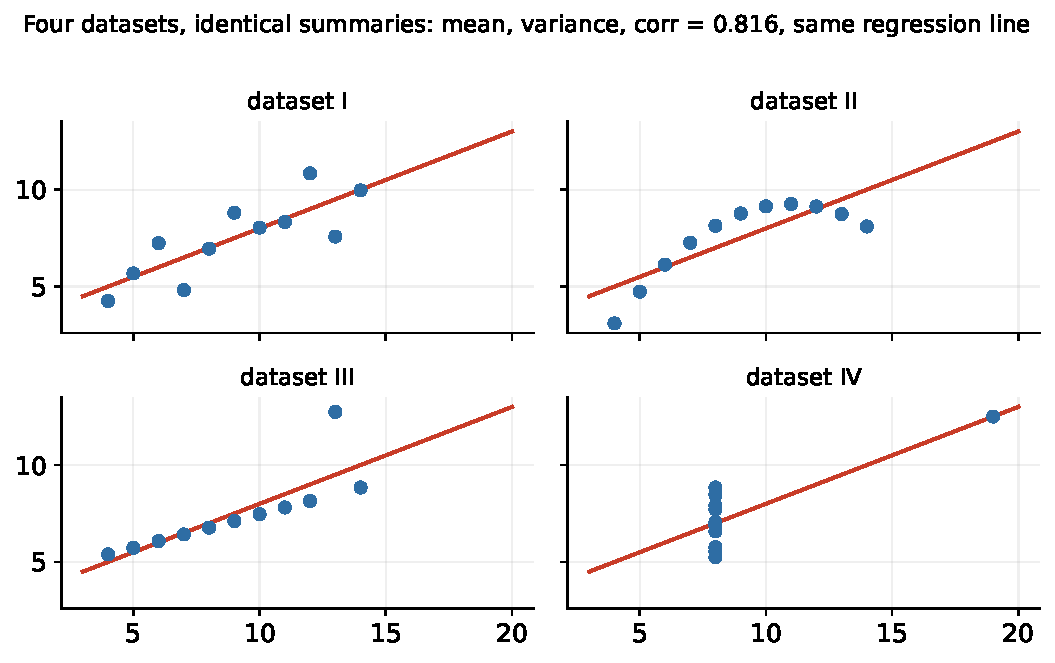
\includegraphics[width=0.7\textwidth]{lecture_1/figures/fig_anscombe.pdf}
\caption{Anscombe's quartet: identical summaries, different data.}
\label{fig:anscombe}
\end{figure}

\subsubsection{Outliers: spot, then decide}
\begin{figure}[htbp]
\centering
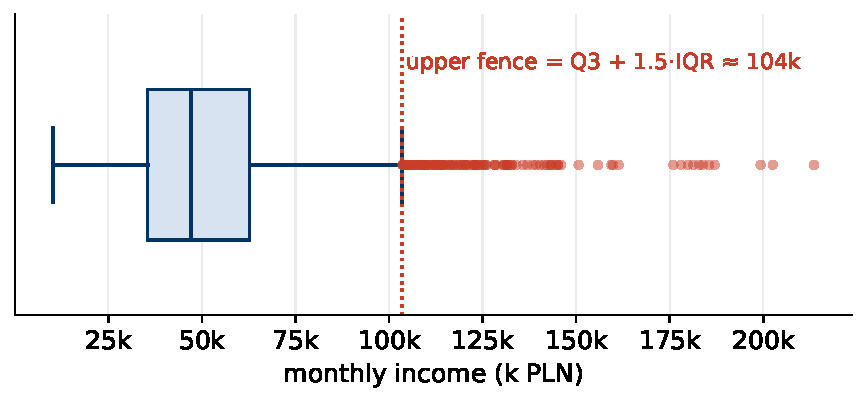
\includegraphics[width=0.78\textwidth]{lecture_1/figures/fig_outliers_box.pdf}
\caption{Income with the IQR fence. Every flagged point here is a genuine
high earner, not an error.}
\label{fig:outliers}
\end{figure}

The boxplot's IQR rule flags points beyond $Q_3 + 1.5\cdot\mathrm{IQR}$
(Figure~\ref{fig:outliers}). It is a convention, not a law: for skewed
variables it flags many perfectly genuine values - log-transform first and
look again. What to \emph{do} about an outlier is a four-step decision, in
order: investigate (error or real?); if an error, fix it at the source or
set it to missing - do not invent a replacement value; if genuine, keep it,
possibly capped (winsorised) or log-transformed so it stops dominating; and
document the rule, because ``we capped income at the 99th percentile'' must
be applied identically to every future dataset the model scores.

\paragraph{Where the $1.5 \times$IQR rule comes from - and when it
misleads.} The magic constant is not magic. For a normal distribution the
quartiles sit at $\mu \pm 0.674\,\sigma$, so the interquartile range is
$\mathrm{IQR} = 1.349\,\sigma$, and the upper fence lands at
\[
Q_3 + 1.5\cdot\mathrm{IQR}
\;=\; \mu + 0.674\,\sigma + 1.5 \times 1.349\,\sigma
\;\approx\; \mu + 2.70\,\sigma .
\]
Under normality about $0.35\%$ of values fall beyond each fence - roughly
$0.7\%$ flagged in total, a pleasantly small ``worth a second look'' pile.
Tukey, who proposed the rule, reportedly chose $1.5$ because $1$ flagged
too much and $2$ too little; it is a calibrated convention for
approximately symmetric data, nothing deeper. Knowing the derivation tells
you exactly when the rule breaks. On \emph{skewed} data the normal
calibration is void: a right-skewed income variable will have a crowd of
genuine values beyond the upper fence (as in
Figure~\ref{fig:outliers}) while the lower fence sits below zero,
flagging nothing - the rule turns into a skew detector, not an outlier
detector, which is why the advice is to log-transform first and look
again. On \emph{heavily discrete} data the rule can degenerate: if more
than half the customers have, say, the same number of existing loans, the
IQR can be tiny or zero and the fences collapse onto the median, flagging
every other value in the column. On \emph{small samples} the quartiles
themselves are noisy, so the fences wobble. And on \emph{mixtures} - two
populations glued into one column, such as retail and private-banking
customers in one income field - the rule flags the smaller population
wholesale, which is a finding about segmentation, not about data errors.
The practitioner's summary: the IQR rule is a cheap tripwire that draws
your attention; the four-step decision above - investigate, fix or keep,
transform, document - is the actual outlier policy.

\begin{practice}
Whether an outlier is a problem depends entirely on the business question.
In fraud detection the outliers often \emph{are} the signal - the analyst
who routinely deletes them is deleting the fraud. The same customer that
distorts an income histogram may be the case your model exists to catch.
\end{practice}

EDA, finally, is a loop, not a phase: ask a question, make the one plot that
answers it, let the answer raise two new questions, and repeat until the
surprises stop. Keep an evidence log - one sentence plus one plot per
finding. ``Income is MNAR-missing for high earners'' is worth more than
forty unlabelled histograms, and your future self will re-read it.

\subsection{Missing data: the anatomy}
\label{sec:missing}
Missing data is where Block 1 earns its keep, because missingness is not one
thing. The \emph{mechanism} behind the gaps decides what treatments are
safe:

\begin{center}\small
\begin{tabular}{@{}lp{5.4cm}p{5.4cm}@{}}
\toprule
Type & Meaning & Example in our portfolio \\
\midrule
\textbf{MCAR} & missing completely at random - unrelated to anything & a form field lost to a system glitch \\
\textbf{MAR} & depends on \emph{observed} data & employment length missing far more often for renters \\
\textbf{MNAR} & depends on the \emph{unobserved} value itself & high earners decline to state income \\
\textbf{Structural} & the value cannot exist & months since last delinquency, when there was none \\
\bottomrule
\end{tabular}
\end{center}

\begin{figure}[htbp]
\centering
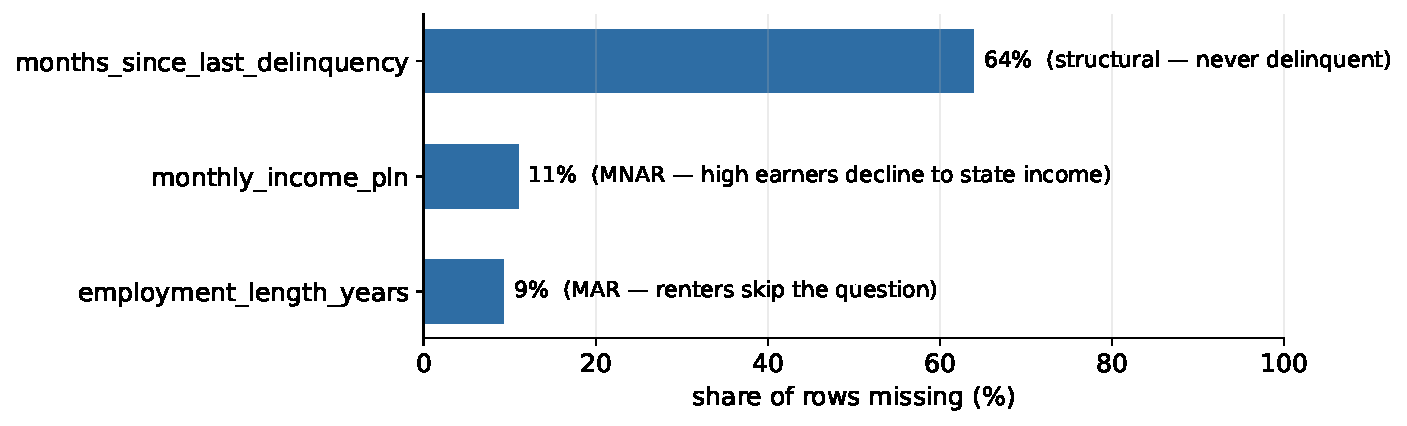
\includegraphics[width=0.86\textwidth]{lecture_1/figures/fig_missingness.pdf}
\caption{Missingness in the course portfolio: three columns, three
mechanisms, three different correct treatments.}
\label{fig:miss}
\end{figure}

Our portfolio exhibits three of the four (Figure~\ref{fig:miss}), and the
lab notebook finds evidence for each. The MAR case is directly checkable:
group the missingness indicator of employment length by housing status, and
renters show a $\sim$16\% missing rate against $\sim$4\% for owners - the
missingness depends on an \emph{observed} column. The MNAR case is subtler,
and this is the uncomfortable truth about MNAR in general: it is invisible
in principle, because the missingness depends on the value we never see. It
can, however, leave fingerprints on correlated, observed variables. Savings
correlate with income; in our data, customers with missing income show a
median savings balance of about 3{,}000 PLN against about 2{,}400 for the
rest - indirect evidence that the unstated incomes were high. No
statistical test proves MNAR from observed data alone; the diagnosis comes
from proxies like this plus domain knowledge (wealthy applicants often
decline to state income).

\subsubsection{Rubin's formalism, in plain mathematics}
The MCAR/MAR/MNAR taxonomy comes from Rubin (1976), and its formal version
is worth thirty seconds because it makes precise what the table above says
loosely - and because it explains, rather than merely asserts, why the
mechanism dictates the treatment. Write $Y$ for the complete data we wish
we had (all features and the target, for every customer), split it into
the part we actually observe, $Y_{\mathrm{obs}}$, and the part that is
missing, $Y_{\mathrm{mis}}$, and let $M$ be the missingness indicator -
a matrix of the same shape as the data with $M_{ij}=1$ where value $j$ of
row $i$ is missing. The mechanism is the conditional distribution
$P(M \mid Y_{\mathrm{obs}}, Y_{\mathrm{mis}})$: how does the pattern of
gaps depend on the data? The three cases are three assumptions about this
distribution:
\[
\textbf{MCAR:}\quad
P(M \mid Y_{\mathrm{obs}}, Y_{\mathrm{mis}}) \;=\; P(M),
\]
the gaps depend on nothing - a coin flip decides who answers;
\[
\textbf{MAR:}\quad
P(M \mid Y_{\mathrm{obs}}, Y_{\mathrm{mis}}) \;=\;
P(M \mid Y_{\mathrm{obs}}),
\]
the gaps may depend on what we \emph{did} observe (renters skip the
employment field more often - and housing status is on file), but given
the observed data, they carry no further information about the missing
values themselves;
\[
\textbf{MNAR:}\quad
P(M \mid Y_{\mathrm{obs}}, Y_{\mathrm{mis}})
\text{ genuinely depends on } Y_{\mathrm{mis}},
\]
the gap depends on the value hiding inside it - high earners decline to
state income \emph{because} it is high. Structural missingness sits
outside the trio: there $Y_{\mathrm{mis}}$ does not exist even in
principle, so the question ``what would the value have been?'' has no
answer to estimate.

Two consequences follow directly from the definitions. First, MAR is the
weakest assumption under which the missing values can be handled by
looking only at observed data: under MAR, everything the gaps could tell
us about the missing values is already carried by the observed columns,
so methods that condition on those columns (group-wise or model-based
imputation, likelihood methods) are on solid ground. Under MNAR the gaps
carry information that no observed column can recover, and any method
pretending otherwise is quietly assuming MAR. Second - and this is the
uncomfortable part - the distinction between MAR and MNAR is
\emph{untestable from the observed data alone}: both mechanisms can
produce identical observed datasets. You can test MCAR against MAR (our
16\%-versus-4\% grouping does exactly that, and rejects MCAR), but the
MAR-versus-MNAR verdict always rests partly on domain knowledge, which is
why the income diagnosis above leaned on the savings proxy \emph{plus} an
argument about applicant behaviour.

\paragraph{Why the mechanism dictates the estimator: a worked miniature.}
Abstract definitions become believable when you watch a simple estimator
fail. Toy numbers, arranged around our MAR example. Suppose a portfolio is
60\% homeowners and 40\% renters, owners earn 7{,}000 PLN a month on
average and renters 4{,}000, so the true average income is
$0.6 \times 7{,}000 + 0.4 \times 4{,}000 = 5{,}800$. Now let the
employment-style MAR mechanism act on income instead: owners fail to state
income 4\% of the time, renters 16\% of the time (the chapter's observed
missingness rates, borrowed for the toy). Compute the naive complete-case
average - the mean over rows where income is present. The owners
contribute $0.6 \times 0.96 = 0.576$ of the original population, the
renters $0.4 \times 0.84 = 0.336$; among complete cases the owner share
has risen to $0.576/0.912 \approx 0.632$. The complete-case mean is
therefore about
$0.632 \times 7{,}000 + 0.368 \times 4{,}000 \approx 5{,}896$ - biased
upward, because deletion silently reweighted the sample toward the
better-earning group. The bias is small here because the missingness
rates are moderate; make the mechanism stronger and it grows without
bound. Notice also what repairs it: within each housing group the data is
(by assumption) missing at random, so the group means are unbiased, and
recombining them with the \emph{true} group weights
($0.6$ and $0.4$, which we know, because housing is observed) recovers
5{,}800 exactly. That is the MAR recipe in miniature - condition on the
observed variables that drive the missingness, and the damage is undone;
ignore them, and every ``simple'' summary inherits a tilt. Under MNAR no
observed variable carries the needed information, and no reweighting or
imputation built from observed data can fully repair the bias - which is
precisely why the taxonomy matters before any treatment is chosen.

A missingness \emph{matrix} - rows as customers, columns as variables,
gaps in white - shows the structure at a glance: which columns, how often,
and whether gaps co-occur in the same rows
(Figure~\ref{fig:missmatrix}). No dedicated library is needed;
\texttt{df.isna()} is the whole trick.

\begin{figure}[htbp]
\centering
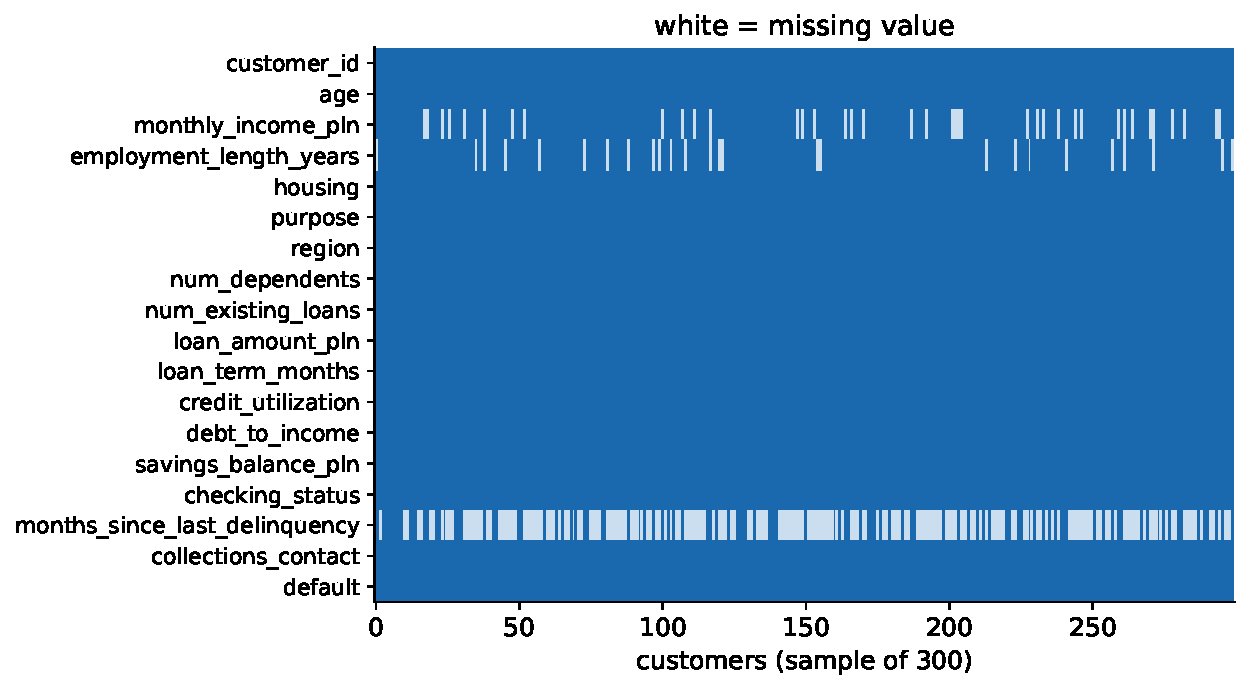
\includegraphics[width=0.72\textwidth]{lecture_1/figures/fig_missing_matrix.pdf}
\caption{Missingness matrix for a 300-customer sample.}
\label{fig:missmatrix}
\end{figure}

\subsubsection{Deletion, and when it is (not) safe}
The simplest treatment is to drop rows with gaps (listwise deletion). Under
MCAR this is safe-ish: you lose statistical power but introduce no bias.
Under MAR or MNAR it biases the sample toward whoever answers the question.
In our portfolio, dropping the income-missing rows would remove
disproportionately wealthy customers - the median savings of the removed
group is visibly higher - so the surviving ``complete'' dataset
systematically under-represents high earners. Dropping a mostly-empty
\emph{column} is defensible only when it also carries no signal, and both
conditions must be checked: our delinquency column is $\sim$64\% missing and
still among the most informative variables in the data. Deletion is a
modelling decision, not housekeeping; justify it like one.

There is also a compounding cost that the per-column view hides: listwise
deletion drops a row if \emph{any} of its columns is missing, so modest
per-column gaps multiply into a large row-level loss. As a toy
illustration, ten columns that are each independently missing for 5\% of
customers leave only $0.95^{10} \approx 60\%$ of rows fully complete -
you would discard four rows in ten to avoid handling gaps that
individually looked negligible. Real missingness is usually correlated
across columns (the same customers skip several fields), which softens the
arithmetic, but the direction of the lesson stands: deletion is priced per
row, not per gap, and the price grows with the width of the table.

\subsubsection{The imputation menu}
\begin{center}\small
\begin{tabular}{@{}lp{5.2cm}p{5.2cm}@{}}
\toprule
Method & Good & Risky \\
\midrule
Mean / median & simple, fast; median survives skew & shrinks variance; distorts under MAR/MNAR \\
Mode (categorical) & simple & inflates the majority level \\
Group-wise median & respects segments (e.g.\ per region) & groups must be big enough \\
Model-based / KNN & uses relationships between features & complexity; leakage risk if fitted on all data \\
Constant + \textbf{indicator} & keeps ``was missing'' as signal & adds columns \\
\bottomrule
\end{tabular}
\end{center}

One golden rule spans every row of the menu: any imputation with fitted
parameters (a mean, a median, a model) must be fitted on the \emph{training
data only} and then applied to the test data - otherwise information leaks
across the split. This is a preview of Block~3's leakage discussion.

\paragraph{Why the indicator works.} The ``constant + indicator'' row
deserves a mechanical explanation, because it looks like a hack and is in
fact the honest option. Adding a 0/1 column \texttt{was\_missing} lets any
downstream model treat the missing group as its own segment: a linear
model gains a separate intercept shift for rows with the gap, a tree can
split on the indicator directly. In effect the model estimates ``the
default rate given that this field is absent'' as a quantity in its own
right - which is exactly the right target, because at scoring time future
applicants will arrive with the same kinds of gaps, and the model must
say something sensible about them. This is also where \emph{prediction}
parts company with classical \emph{inference}. For estimating a
population parameter, MNAR missingness is a wound that observed data
cannot fully heal. For prediction, the question is milder: we only need
$P(\text{default} \mid \text{what we observe})$, and ``this field is
missing'' is itself an observable fact. The indicator turns the gap into
data, and the model conditions on it like on any other feature - valid
under any mechanism, MNAR included, with one condition attached: the
missingness process must be \emph{stable} between training and
deployment. If the application form changes and a field that used to be
optional becomes mandatory, the indicator's meaning evaporates overnight
- one more reason data provenance belongs in your documentation.

\paragraph{Multiple imputation - an honourable mention.} The statistics
literature's gold-standard answer to missing data is \emph{multiple
imputation}: instead of filling each gap with one number, draw several
plausible values from a model of the missing data given the observed
data, produce $m$ completed datasets, run the analysis on each, and pool
the results (with rules, due again to Rubin, that combine
within-imputation and between-imputation variability). Its virtue is
honesty about uncertainty: a single-value imputation pretends the gap is
known, and every downstream standard error is too small; multiple
imputation propagates ``we are not sure what this value was'' into the
final answer. It is standard practice in medical and social-science
inference. In production credit scoring it is rare - a deployed
scorecard needs one deterministic score per applicant, not a
distribution of scores - so industry practice leans on the
indicator-plus-impute pattern instead. Know that multiple imputation
exists, know what problem it solves (uncertainty, not prediction), and
reach for it when your goal is an estimate with an honest confidence
interval rather than a scoring pipeline.

\subsubsection{The punchline: a missing value can be a signal}
\begin{figure}[htbp]
\centering
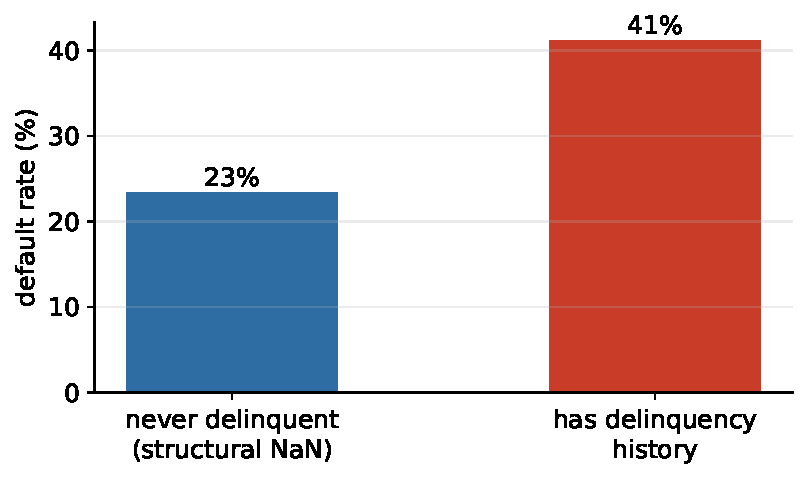
\includegraphics[width=0.5\textwidth]{lecture_1/figures/fig_structural_signal.pdf}
\caption{Default rate by presence of the structural gap: never-delinquent
customers (NaN) versus customers with a delinquency history.}
\label{fig:signal}
\end{figure}

The structural gap in \texttt{months\_since\_last\_delinquency} is the
centrepiece of the block. Customers with the NaN - who were never
delinquent - default at about 23\%; customers with a real value default at
about 41\% (Figure~\ref{fig:signal}). The \emph{fact} of missingness is
itself one of the strongest predictors in the dataset.

Now watch what naive mean imputation does. The observed values average about
31 months, so imputation assigns every never-delinquent customer a synthetic
delinquency roughly 31 months ago. Two very different groups now carry the
same feature value: the genuinely delinquent customers with values near the
mean default at about 40\%, the imputed never-delinquents at about 23\% -
and the model can no longer tell them apart. In the lab, the model-free
quantification is stark: the mean-imputed column's correlation with default
is $0.02$; the missing-\emph{indicator}'s is $-0.19$. Nearly all the signal
lives in the gap, and imputation erased it. The honest first move is
therefore: add a missing-indicator column, \emph{then} impute the number.

\paragraph{The economics of missingness-as-signal.} Why should the
\emph{absence} of a number predict anything? Because in business data,
gaps are rarely accidents of measurement - they are the traces of
decisions, and decisions are made by people with information. The
delinquency NaN encodes a clean credit history: here the absence of a
record \emph{is} the record, and it is the single most valuable fact a
lender can know about repayment behaviour. The income gap has a different
economics - self-reported fields are subject to a mild form of adverse
selection, where what a customer chooses not to disclose correlates with
what the disclosure would reveal; the same logic makes ``no checking
account'' (Figure~\ref{fig:checking}) informative, since it deprives the
bank of exactly the cash-flow visibility that reassures it. Once you see
gaps as traces of processes, you also see the caveats. Some
missingness patterns encode the \emph{pipeline} rather than the customer
- applications arriving through a broker channel may lack fields the
branch form collects, so the indicator quietly becomes a channel flag,
predictive today and gone after the next IT release. And an indicator can
proxy for things a lender must not use: if declining to state a field
correlates with a protected characteristic, the ``signal'' walks the
model into fairness territory that Block~6 treats seriously. The craft
position: harvest missingness as signal deliberately - indicator first,
impute second - but document what each indicator most likely
\emph{means}, and treat an indicator whose meaning you cannot explain as
a risk, not a free lunch.

\begin{practice}
In regulated lending this is not merely a modelling nicety. Adverse-action
reasons given to a declined customer must be truthful. ``You were declined
because of a delinquency 28 months ago'' would be a false statement about a
customer who was never delinquent - an invented history, manufactured by
an imputation default. Imputation choices are not cosmetic; they change the
story the institution tells about a person.
\end{practice}

\subsection{Feature engineering: a first look}
\label{sec:fe}
Feature engineering is the craft of building new columns that expose
structure a model would struggle to find alone - the step of CRISP-DM's
\emph{data preparation} phase where domain knowledge becomes signal. The
missing-indicator of the previous section \emph{is} feature engineering; the
wider toolbox consists of five recurring moves:

\begin{center}\small
\begin{tabular}{@{}llp{5.2cm}@{}}
\toprule
Move & Recipe & Portfolio example \\
\midrule
Ratio & divide two raw columns & instalment / income \\
Flag & boolean condition & \texttt{has\_delinquency\_history} \\
Binning & continuous $\to$ bands & utilisation: low / mid / maxed-out \\
Interaction & combine two features & renter \emph{and} no checking account \\
Date arithmetic & differences, tenures & months since last delinquency \\
\bottomrule
\end{tabular}
\end{center}

Look at the portfolio's data dictionary again with this table in mind:
\texttt{debt\_to\_income} is a ratio - someone engineered it before us.

\subsubsection{Why ratios beat raw pairs - especially for linear models}
The ratio row of the table is the workhorse of credit features
(debt-to-income, utilisation, instalment-to-income, loan-to-value), and
there is a precise reason it earns its keep. Affordability is inherently
\emph{relative}: a 1{,}500 PLN monthly instalment is a heavy burden on a
3{,}000 PLN income (half of it) and a light one on a 15{,}000 PLN income
(a tenth). The risk-relevant quantity is the quotient, not either raw
number. Now consider what a linear model - the family we meet in
Block~2 - can express with the raw pair: a score of the form
$a \cdot \text{instalment} + b \cdot \text{income} + c$. Whatever weights
you choose, the instalment's contribution to the score is the same
$a \cdot 1{,}500$ for both customers above; the income term shifts their
scores apart, but it cannot make the \emph{effect of the instalment
depend on the income} - that would require a product or quotient of the
two inputs, which is exactly the nonlinearity a linear form excludes.
Handing the model the ratio $\text{instalment}/\text{income}$ as a column
supplies that nonlinearity ready-made, in one interpretable number, and
turns an unlearnable relationship into a single well-behaved slope. This
is the general shape of good feature engineering: you spend domain
knowledge to buy the model a coordinate system in which the true
relationship becomes simple. Flexible models blunt but do not remove the
argument - a deep tree ensemble can approximate a ratio threshold with a
staircase of axis-aligned splits, at the price of many splits and shakier
extrapolation - and in regulated lending the interpretable ratio wins on
explainability grounds anyway. Two cautions for the craft: guard the
denominator (a zero or near-zero income makes the ratio explode - decide
the convention and document it), and keep the raw columns in view during
EDA even if the model only sees the ratio, because errors are easier to
spot in raw units.

\paragraph{Interactions, by the same logic.} The interaction move is the
categorical sibling of the ratio. An additive model forced to score
``renter'' and ``no checking account'' separately must give the
combination the sum of the two individual effects - it has no way to
express ``the combination is worse than the sum of its parts''. An
explicit interaction column (the boolean AND of the two flags) grants
exactly that freedom, one column at a time, guided by domain sense about
\emph{which} combinations plausibly matter. The worked example below shows
the payoff on our portfolio.

\paragraph{A worked example.} Renting alone is mildly risky (34\% default
against the 30\% portfolio average), and having no checking account alone is
similar (35\%). The \emph{interaction} flag - renter \emph{and} no
checking account - isolates a segment defaulting at 39\%, on $n=318$
customers, comfortably enough to trust (Figure~\ref{fig:interaction}). Two
weak signals, combined by domain sense, concentrate into a strong one. And
the strongest engineered feature of the whole block is one we built in
Section~\ref{sec:missing} without calling it that: the
\texttt{delinq\_missing} indicator, whose correlation with default
($|r| \approx 0.19$) exceeds that of any raw numeric column in the data.

\begin{figure}[htbp]
\centering
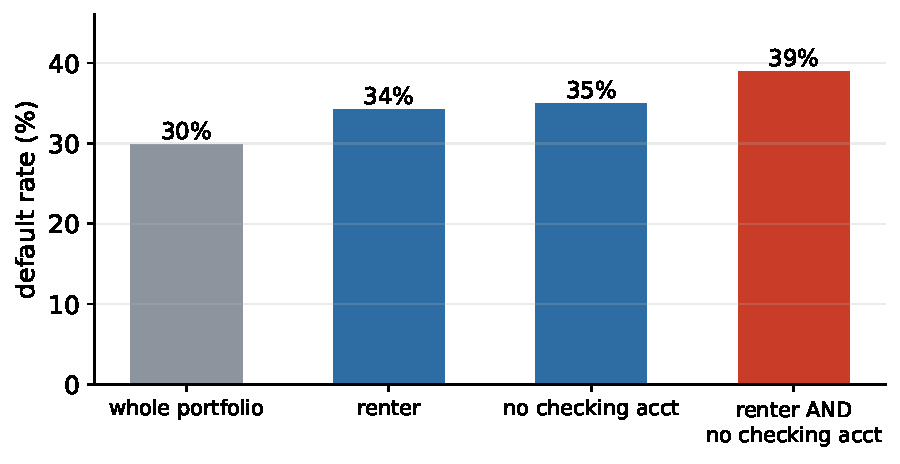
\includegraphics[width=0.56\textwidth]{lecture_1/figures/fig_interaction.pdf}
\caption{Combining two weak flags isolates the riskiest segment.}
\label{fig:interaction}
\end{figure}

\paragraph{Encodings: making categories digestible.} Most models eat
numbers, not labels, so categorical features must be encoded - and the
scale of measurement picks the encoding. \emph{One-hot encoding} (one 0/1
column per level) is the safe default for nominal variables like purpose or
region; its cost is column explosion when a variable has many levels.
\emph{Ordinal codes} (none $=0$, low $=1$, \ldots) are right exactly when
the order is real, as for checking status - and wrong otherwise, because
they invent distances. \emph{Target encoding} (replacing a level by the
average target within it) handles high-cardinality nominals elegantly and
is a leakage machine when fitted on all data - it must be fitted on the
training split only, one more instance of Block~3's golden rule. Credit
scoring's own tradition is \emph{Weight of Evidence} (WoE): bin a feature,
then encode each bin by $\ln(\%\text{good}/\%\text{bad})$; it pairs
naturally with scorecards and returns in Block~2. Encoding choices look
mechanical but change what a model can learn - scale first, encoding
second.

\paragraph{Why target encoding is dangerous: a five-row disaster.} The
target-encoding warning deserves its own toy example, because the failure
is subtle enough to survive code review. Suppose the loan-purpose column
contains a rare level - say, ``boat'' - with just two customers in the
data, and both happened to default. Naive target encoding replaces
``boat'' with the level's observed default rate: $2/2 = 1.0$. The model
now receives a feature announcing that boat purchasers default with
certainty - a ``fact'' manufactured from two data points, i.e.\ from
noise. Worse, if the encoding was computed on \emph{all} rows before the
train/test split, the test-set boat customer's own outcome is baked into
the feature value used to predict that same outcome - the model is shown
the answer in disguise, and cross-validation will cheerfully report a
score the model can never achieve on genuinely new data. Two standard
repairs, both worth knowing by name. \emph{Smoothing} shrinks each
level's rate toward the global prior in proportion to how little data the
level has: with the formula
$(n \cdot \text{rate} + k \cdot \text{prior})/(n + k)$ and a prior
strength of $k=20$, the boat level's encoding becomes
$(2 \times 1.0 + 20 \times 0.3)/22 \approx 0.36$ - pulled firmly back
toward the portfolio's 30\% base rate, as two observations deserve.
\emph{Out-of-fold fitting} computes each row's encoding from data that
excludes that row's fold, so no row's own target ever touches its own
feature. Used with both repairs and fitted on the training split only,
target encoding is a respectable tool for fifty-level categoricals; used
naively, it is the single most common source of the too-good-to-be-true
scores that Block~3 teaches you to distrust.

Two rules discipline the craft. First, every engineered feature must pass
the \emph{time-travel test} (Section~\ref{sec:leakage}): it may use
application-time information only. Second, any transform with fitted
parameters - bin edges, scaling means, encodings - must be fitted on the
training data only; this is the leakage-safe pipeline of Block~3. In
regulated lending a third constraint joins them: features must remain
explainable, because any of them may end up in an adverse-action reason.
Expect diminishing returns - five features built from domain sense
routinely beat five hundred generated blindly - and document every recipe,
because production must compute the feature \emph{identically} or the model
silently degrades.

Feature engineering runs through the whole course rather than owning one
block: missing-value indicators here, encodings for regression in Block~2,
leakage-safe pipelines in Block~3, and turning raw text into a feature
matrix in Block~5.

\subsection{A first warning about leakage}
\label{sec:leakage}
Leakage is using information at training time that will not exist at
prediction time. Our dataset carries a deliberate example:
\texttt{collections\_contact} records whether the collections department
contacted the customer - which happens mostly \emph{after} default. A
model given this column looks brilliant in the notebook and is worthless in
production, because at application time the collections call has not
happened yet.

The universal antidote is the \emph{time-travel test}, asked of every
feature, raw or engineered: \emph{would I have known this value at the
moment of the decision?} If the answer is no, the feature is a time
traveller; drop it. Block~3 stages a live demonstration - training with
and without the leaky column - and generalises the test to subtler forms
of leakage (duplicates across the train/test split, transforms fitted on all
data, target information smuggled through encodings).

\paragraph{Making the test a discipline, not a vibe.} Asked casually, the
time-travel test catches only the obvious offenders; the subtle ones
require it to be asked \emph{per column, in writing}. The working form is
a feature inventory: one row per candidate feature, recording what the
value means, which system it comes from, and - the load-bearing entry -
\emph{at what moment the value becomes known and frozen}. Filling in that
last column is where the quiet time travellers surface. A ``current
balance'' field extracted from an operational system is current as of the
\emph{extraction} date, not the application date - for a two-year-old
application it embeds two years of the future. A customer table that is
updated in place (address, employment, income corrected over time) shows
you today's version of yesterday's applicant. An aggregate like ``average
utilisation over the last 12 months'', computed once over the whole
dataset, spans the outcome window for early applications. None of these
columns is labelled ``leak''; each is discovered only by asking, pedantically,
when its value was written. Hence the discipline: no feature enters the
modelling table without a stated as-of time, and any feature whose as-of
time cannot be established is treated as leaky until proven otherwise -
the burden of proof sits with the feature, not with the doubter. The
inventory feels bureaucratic on a 18-column teaching portfolio; on a
production system with hundreds of candidate columns from a dozen source
systems, it is the difference between an audit and an incident.

\subsection{The craft: habits that save beginner data scientists}
Beyond methods, Block 1 closes with the working habits that distinguish
reliable analysts. Each of these exists because of a common, expensive
failure mode.

\paragraph{Reproducibility from day one.} Fix random seeds everywhere a coin
is flipped (splits, models, samples). Pin the environment - the course
repository ships a \texttt{uv} lockfile; ``works on my machine'' is not a
result. Follow the one-command rule: a colleague should reproduce your
numbers by running one thing top to bottom. Record data provenance -
where the data came from and when, because datasets change under your feet.
If it cannot be reproduced, it is an anecdote, not an analysis - and the
project rubric scores it.

Why so much ceremony for a student project? Because every element answers
a failure you will otherwise meet personally. Unseeded randomness means
your headline number changes each run, and you cannot tell an improvement
from a reroll - the seed converts ``the score moved'' into ``my change
moved the score'', which is the only comparison worth making. Unpinned
environments mean a teammate installs a newer library version and gets
different results from identical code; the lockfile makes the environment
part of the analysis, versioned like the code. Unrecorded provenance
means that when the source data is refreshed - and business data is
refreshed constantly - nobody can say whether today's disagreement with
last month's numbers is a bug or a data change. And the one-command rule
is ultimately a social contract: it is the difference between ``trust
me'' and ``check me'', and in any serious setting - a regulator, a model
validator, a co-author, your own team six months later - only the second
is acceptable. Reproducibility is cheap when built in from the first
commit and painfully expensive to retrofit; day one is the discount
window.

\paragraph{Notebooks: superpower and trap.} Notebooks put code, plots and
narrative in one place, which makes them perfect for EDA and for the course
project. Their trap is hidden state: cells run out of order produce results
that cannot be recreated, and deleted cells leave live variables behind. The
habit that saves you: before trusting any result, \textbf{Restart kernel \&
run all}. If it breaks, it was already broken - you just did not know.

\paragraph{Version control - yes, for analysts too.} Commit small and
often, with messages that say why. Code, notebooks, configs and figure
scripts go in; raw data (use loaders), credentials and hundred-megabyte
artefacts stay out. In a student project the payoff is concrete: at 23:50
before the deadline you will want yesterday's working version back.

\paragraph{Reading errors and asking good questions.} Read tracebacks
bottom-up - the last line is the error, the lines above are where it
happened. Reproduce the bug in the smallest possible example; half the time
it evaporates as you shrink it. When asking for help (a colleague, a forum,
an AI assistant), state what you expected, what happened instead, and what
you tried, with the minimal example attached. The discipline of writing the
question well often answers it.

\paragraph{Communicating to humans.} Lead with the decision, not the method:
``we can cut losses 12\% at the same approval rate'' beats ``our AUC is
0.79''. State uncertainty honestly - ranges and caveats build trust, false
precision destroys it. One chart, one message. And know your audience: the
risk committee, the regulator and a fellow data scientist need three
different stories. A model's impact is capped by its author's ability to
explain it.

\paragraph{Beginner traps.} Six mistakes account for most early-career
disasters, and the course meets each one deliberately: evaluating on
training data (Block 2); optimising accuracy on a 97/3 problem (Block 3);
reaching for complex models before a baseline, so the extra complexity can
never be judged (Blocks 2 and 6); not looking at the data - Block 1's
whole point; torturing the data until it confesses (testing a hundred
hypotheses and reporting the five that ``worked''); and silently deleting
inconvenient rows, when outliers and missing values carry signal. The course
subtitle is a promise: how not to fool yourself.

\subsection{Lab and hand-in}
The lab notebook \texttt{01\_eda\_missingness} walks the full arc of this
chapter on the live portfolio: first contact and keys; target balance;
univariate shapes, the log lens and sanity checks; bivariate default-rate
plots; correlations and outliers; the missingness taxonomy with evidence for
each mechanism; and the imputation experiment that reproduces the numbers of
Section~\ref{sec:missing}. Five exercises extend it, including engineering
one feature from loan amount, term and income - and defending it.

``Done'' for Block 1 means: you can defend, in one paragraph, how you would
treat each missing column and why. The project-team hand-in is a
one-paragraph \emph{data understanding} note: the target, the class balance,
and the top three data-quality risks you found. A useful self-check before
submitting: for every claim in your paragraph, you should be able to point
at the one plot or one number that backs it - the evidence-log habit of
Section~\ref{sec:eda}, applied to your own work.

% =====================================================================
\section{Block 2 - Regression, re-framed: from inference to prediction}

Block 1 ended with a feature matrix and a promise: this week the features
meet their first models. The models themselves - linear and logistic
regression - you have seen before, in econometrics, and that is precisely
why this chapter exists. The mathematics will be familiar; the
\emph{question asked of it} will not. Econometrics fits a regression to
learn about the world; this course fits the same regression to score the
next applicant. Almost every habit you carry from the first tradition -
staring at p-values, celebrating $R^2$, trusting in-sample fit - must be
re-examined under the second, and some must be unlearned. By the end of
the block you will have a defensible probability-of-default baseline on a
real portfolio, and, more importantly, the discipline that makes the word
``defensible'' mean something: held-out evaluation, honest metrics, and a
threshold chosen by economics rather than habit.

\subsection{Why these models, in the age of LLMs}
A fair question opens the block: large language models exist - why learn
logistic regression? Five reasons, each sufficient on its own. First,
structured data is not language: on tabular problems like a credit
portfolio, small dedicated models still match or beat LLMs, at a millionth
of the cost per decision. Second, explainability is a legal requirement -
a declined customer is entitled to reasons, and ``the LLM said so'' is not
one, while coefficients and odds ratios are. Third, regulation: credit
models live inside model-risk frameworks - validated, monitored, audited,
reproducible - and a deterministic model with fixed coefficients can be
audited in a way a prompt cannot. Fourth, insight: the point is often the
\emph{drivers} rather than the prediction, and a coefficient answers where a
chat completion gestures. Fifth, engineering economics: millions of scoring
calls a day, identical output for identical input, fractions of a cent
each.

It is worth pausing on what ``auditable'' means concretely, because the
word carries the weight of the argument. A validator receiving a logistic
scorecard gets a finite list of inputs, a fixed vector of coefficients,
and a deterministic formula; she can recompute any decision the bank ever
made, test the model on her own held-out sample, check monotonicity
(does risk really rise with delays?), and sign her name to the result. A
validator receiving a prompt and an API key gets none of that: the
weights are not hers to inspect, the vendor may update the model under
her feet, and the same input can, depending on settings, produce
different outputs on different days. Model-risk frameworks were written
by people who had watched opaque models fail expensively; the frameworks
do not forbid complexity, but they price it, and the price of an
unauditable decision engine in retail credit is currently: not
approvable.

None of this makes LLMs irrelevant here. They are excellent
\emph{assistants} - writing pandas code, explaining tracebacks, drafting
documentation (verify what they produce; Block 1's advice on reading errors
applies doubly). They are promising \emph{feature factories}, turning
complaint texts into categories or embeddings that feed a classical model
- Block 5's pipeline, modern edition. What they are not, for regulated,
high-volume, structured decisions, is the decision engine. The division of
labour: LLMs help you build the model; the model makes the decision; you
remain responsible for both.

\subsection{Tools: scikit-learn and the three samples}
scikit-learn is the standard Python library for classical machine learning
and the workhorse of this course. Its one design idea worth the fame: every
model is an \emph{estimator} with the same interface. \texttt{fit(X, y)}
learns parameters from training data; \texttt{predict(X)} outputs numbers or
classes; classifiers add \texttt{predict\_proba(X)} for class probabilities;
preprocessing objects (scalers, encoders) are \emph{transformers} with
\texttt{transform(X)}. The consequence is strategic: swapping logistic
regression for a random forest is a one-line change, which is exactly why
baselines cost nothing to keep. One warning attaches to \texttt{predict}:
for classifiers it silently applies a 0.5 threshold. In credit we almost
always want \texttt{predict\_proba} and our own threshold
(Section~\ref{sec:eval1} explains why).

The uniform interface deserves one more sentence of appreciation, because
it encodes a methodological stance, not just a convenience. By forcing
every model behind the same three verbs, sklearn makes the \emph{model} a
swappable component and the \emph{protocol} - split, fit, judge - the
part you actually author. That inversion is the right mental model for
the whole course: Blocks 2 through 6 change what sits behind
\texttt{fit}, while the evaluation discipline around it stays fixed. A
student who internalises the protocol can adopt any future model family
in an afternoon; a student who memorises one model's API has learned one
model.

Data, meanwhile, plays three roles, and mixing them is how optimism sneaks
into results. The \textbf{training} sample fits the parameters (the
coefficients). The \textbf{validation} sample compares models and tunes
hyperparameters. The \textbf{test} sample delivers the final judgement -
and is touched \emph{once}. Three questions, three datasets: \emph{what are
the coefficients? which model or setting? how good is the winner, really?}
When data is scarce, cross-validation (Block 3) makes the validation role
cheap by rotating it; today's lab tunes nothing, so a simple train/test
split suffices.

Why three samples and not two? Because any dataset that influences a
choice gets optimistically biased as a judge of that choice. The training
data chose the coefficients, so training error flatters the coefficients.
If the same held-out data then chooses the hyperparameters - you sweep
twenty settings and keep the best score - that best score flatters the
winning setting, for the same reason: among twenty noisy numbers, the
maximum is biased upward. Hence the third sample, reserved for the one
question no earlier sample can answer honestly: how good is the final,
frozen model? Each sample is spent the moment it influences a decision;
budgeting them is part of the craft.

\subsection{The real portfolio}
From this chapter on, the modelling work runs on real data: the UCI
\emph{Default of Credit Card Clients} study - 30{,}000 credit-card
clients of a Taiwanese bank, observed in 2005 (Yeh \& Lien), with the
target ``default next month'' at a base rate of 22.1\%. Each client
carries a credit limit, four demographic fields (sex, age, education,
marriage) and six months of behaviour: monthly repayment status, bill
amounts and payment amounts. The course loader
(\texttt{finance\_data.load\_taiwan()}) downloads the file once and caches
it in the repository, so students work offline; the shared feature matrix
(\texttt{taiwan\_features()}) mixes raw application-time columns with the
engineered features of Blocks 1-2 - utilisation (bill over limit),
payment ratio, delay counters. One column is planted and documented:
\texttt{collections\_contact} is injected from the outcome exactly as in
the synthetic portfolio, and Block 3 detonates it on schedule. Block 1's
synthetic portfolio retires to the missingness lab, where it belongs:
real data never labels its missingness mechanisms, and ours did, by
design. Two side notes for completeness: the classic 1{,}000-row German
Credit (Statlog) set remains available through
\texttt{load\_credit(source="openml")} as the historical reference, and
the Kaggle \emph{Give Me Some Credit} competition set - with genuinely
missing income and a real months-since-delinquency column - is
recommended as an optional Block 1 exercise and a project-pool dataset
for teams with Kaggle accounts.

Two properties make this dataset pedagogically ideal. The 22.1\% base
rate is \emph{friendly} imbalance: rare enough that the accuracy trap of
Section~\ref{sec:eval1} bites visibly, common enough that models still
see thousands of positive examples - real loan books at 1--5\% default
rates are harsher, and we will discuss how. And the six months of
repayment behaviour make it a \emph{behavioural} scoring problem, not an
application-scoring one: the strongest predictors are things the customer
\emph{did} (paid late, revolved a balance), not things the customer
\emph{is} (age, marital status). That ordering - behaviour beats
demographics - is one of the most robust empirical regularities in
retail credit, and you will watch it emerge from the coefficients within
the hour.

\subsection{From inference to prediction}
Students meet regression twice in their education, with different
loyalties. Econometrics asks whether $\hat\beta_1$ is significant and what
its causal story is; prediction asks how accurate $\hat{y}$ is on customers
never seen before. Same fitted coefficients, different success criteria.
This course sits on the prediction side, while borrowing econometrics'
discipline about interpretation - and both traditions share the question
``can I defend this model to a regulator?''

\subsubsection{Shmueli's argument: to explain or to predict}
The cleanest statement of the divide is Shmueli's paper \emph{To Explain
or to Predict?} (Statistical Science, 2010), on the block's reading list
and worth your evening. Its central, initially uncomfortable claim: the
best explanatory model and the best predictive model are, in general,
\emph{different models} - not because one camp is sloppy, but because
the two goals decompose error differently. For a new observation, the
expected squared prediction error splits into three parts:
\[
  \underbrace{\sigma^2_{\varepsilon}}_{\text{irreducible noise}}
  \;+\;
  \underbrace{\text{bias}^2}_{\text{wrong functional form}}
  \;+\;
  \underbrace{\text{estimation variance}}_{\text{finite-sample wobble of }\hat\beta} .
\]
Explanation cares almost exclusively about the bias term: a mis-specified
model gives wrong structural conclusions, full stop. Prediction cares
about the \emph{sum} of the last two terms - and they trade off. Adding
the theoretically correct but weakly identified variable removes a sliver
of bias while adding a slab of estimation variance; dropping it biases
the model and \emph{improves} its predictions. A deliberately
mis-specified model can therefore out-predict the true one, and with
noisy features and modest samples it routinely does. This is not a
paradox; it is the bias-variance trade-off wearing its formal clothes,
and it licenses everything this chapter later does on purpose -
shrinking coefficients toward zero (regularisation) is nothing but
deliberately buying bias to sell variance.

The same argument dethrones the standard error. A standard error
quantifies uncertainty about a \emph{coefficient} - useful when the
coefficient is the product. When the prediction is the product, the
relevant uncertainty is the error of $\hat y$ on new data, and the two
are not interchangeable. With our 30{,}000 rows, utterly negligible
effects clear the 5\% significance bar easily - significance is a
statement about sample size as much as about the world - while a
significant coefficient can add exactly nothing to out-of-sample
accuracy if its information is already carried by other features.
Conversely, prediction has no objection to a coefficient whose sign
makes no causal sense, so long as it helps on held-out data (we will
meet exactly such a coefficient in the logistic baseline). The
practical rule: p-values answer ``is this effect distinguishable from
zero in this sample?''; they do not answer ``will this model score
tomorrow's applicants well?''. This block builds the machinery that
does.

\subsubsection{The golden rule and the split protocol}
Prediction's first principle is the golden rule: \emph{never judge a model
on the data it was fitted on}. A model that reproduces its training data
has proven only that it can memorise; the product we sell is
\emph{generalisation}. The minimum honest protocol is the train/test split:
split once (say 70/30), fit the model and every transform on the training
part only, judge on the test part, and touch the test set as rarely as
possible. Details that bite in practice: stratify classification splits so
the default rate matches in both halves; fix the random seed for
reproducibility; remember that a duplicate landing on both sides of the
split is leakage (Block 1's keys check just became modelling advice); and
with time-stamped data, split by time, not at random (Block 3).

\subsubsection{What the test score actually estimates}
It pays to be precise about what the test number \emph{is}, because the
precision changes how you read it. The quantity we care about is the
generalisation error: the expected loss of our frozen model on a fresh
customer drawn from the same population. That is a population quantity we
can never observe. The test score is its \emph{estimator}: an average of
losses over the particular customers who happened to land in the test
set. Like every estimator, it has sampling variance - re-deal the split
and the number moves. How much? For accuracy the arithmetic is
back-of-envelope binomial: a score of about $0.8$ on $9{,}000$ test rows
has standard error $\sqrt{0.8 \times 0.2 / 9000} \approx 0.004$, so the
honest reading of ``80.6\%'' is ``80.6\%, give or take roughly $0.4$
percentage points; a 95\% interval is about $\pm 0.8$ points''. Three
consequences follow. First, differences in the third decimal place
between two models on a test set this size are noise, not ranking -
resist the leaderboard instinct. Second, small test sets give noisy
verdicts: a 300-row test set has a standard error near $2.3$ points, wide
enough to reverse most model comparisons; this is one reason Block 3's
cross-validation, which averages several held-out estimates, is worth
its cost. Third, the estimator is unbiased \emph{only if} the test set
never influenced any choice - which is exactly why the peeking rule
below exists, and why ``we picked the model that did best on test'' is a
confession, not a methodology.

\begin{figure}[htbp]
\centering
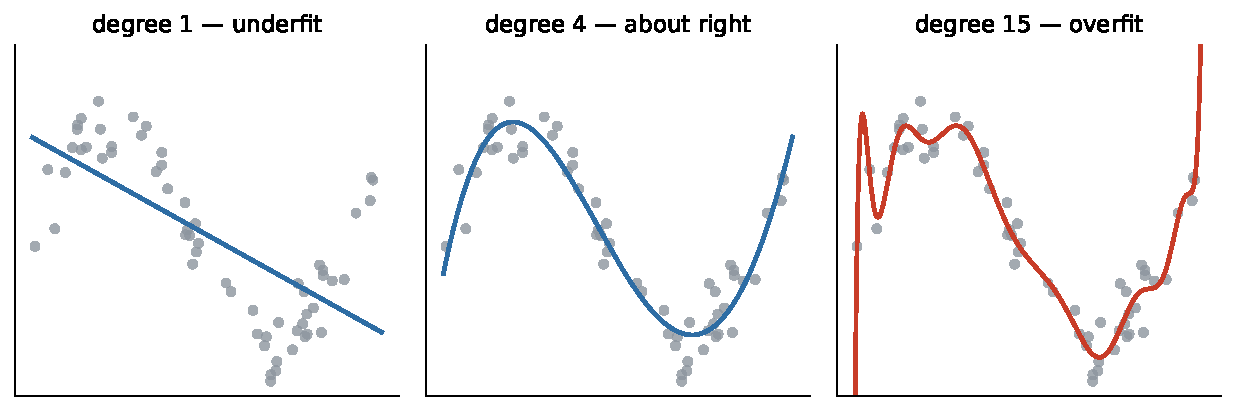
\includegraphics[width=0.86\textwidth]{lecture_2/figures/fig_overfitting.pdf}
\caption{One dataset, three polynomial fits: underfit, about right, overfit.
The overfit curve fits the \emph{training} points best - exactly why
training error cannot be trusted.}
\label{fig:overfit}
\end{figure}

Figure~\ref{fig:overfit} shows why the rule exists. The degree-15
polynomial hugs the training points more closely than the sensible
degree-4 fit - and predicts worse everywhere between them. Sweep the
complexity dial and the pattern generalises into
Figure~\ref{fig:ucurve}: training error falls monotonically with
complexity, while test error traces a U - underfitting on the left,
overfitting on the right. Model selection means finding the bottom of that
U without peeking at the test set; regularisation
(Section~\ref{sec:regularisation}) is one steering wheel for it.

\subsubsection{The U-curve worked in numbers}
The U-curve deserves one pass in explicit numbers, because the picture
alone lets you nod along without feeling the mechanism. Set up a toy
problem: ten observations $(x_i, y_i)$ generated from a gently curved
truth - say a quadratic in $x$ - plus noise with variance 1. Now fit
polynomials of increasing degree and count parameters. A degree-1 fit
spends 2 parameters; it cannot bend, so its training error contains both
the noise \emph{and} a bias term from the missed curvature. A degree-2
fit spends 3 parameters, matches the truth's shape, and its training
error settles near the noise floor of 1 - it cannot honestly go lower,
because the remaining scatter is genuinely random. A degree-9 fit spends
10 parameters on 10 points, and here a small algebraic fact does the
teaching: a polynomial of degree $n-1$ through $n$ points can
\emph{interpolate} them exactly. Training error: precisely zero. Zero!
And precisely uninformative - the fit has spent its entire budget
memorising the noise, and between the training points it swings through
wild excursions to honour each memorised wiggle. On fresh data from the
same truth, a representative run of this experiment reads roughly:
degree 1, training error $4$, test error $4.5$ (biased both sides);
degree 2, training $0.9$, test $1.2$ (near the irreducible floor);
degree 9, training $0.0$, test in the hundreds. The numbers vary run to
run; the shape never does. Two morals to carry out of the toy. Training
error is a \emph{biased} estimator of generalisation error, and the bias
grows with model flexibility - at the interpolation extreme the training
score contains no information at all. And the bottom of the test-error U
sits where the model is just flexible enough for the structure and no
more; every parameter past that point is purchased with test error.

\begin{figure}[htbp]
\centering
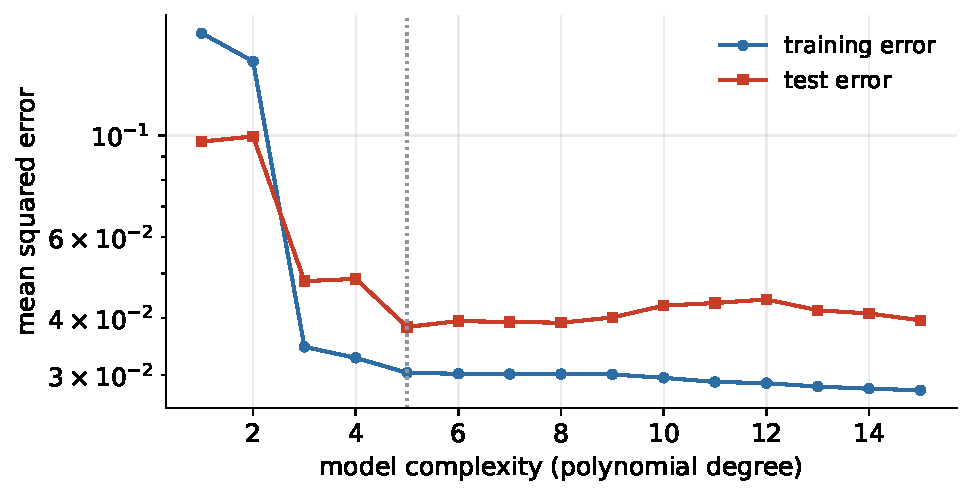
\includegraphics[width=0.6\textwidth]{lecture_2/figures/fig_bias_variance.pdf}
\caption{Training and test error versus model complexity. The test-error U
is the central picture of applied machine learning.}
\label{fig:ucurve}
\end{figure}

Two more self-deceptions complete the set. \emph{Extrapolation}: a model is
trustworthy inside the range of its training data; our portfolio's incomes
top out around 1M NT\$, so for a 5M NT\$ applicant the model will output a
number confidently and baselessly - and Block 1's selection bias makes
this worse, since the training data contains approved customers only.
\emph{Test-set peeking}: check the test score, tweak, check again - after
a dozen rounds you have manually fitted the test set and its verdict is
contaminated. The test set answers one question, once, at the end.
Peeking is worth spelling out mechanically, because nobody plans to do
it. You fit model A, check the test score, feel dissatisfied, add a
feature, check again, remove an outlier, check again. Each check was
innocent; the sequence was not. You have run an informal search whose
objective function was the test score, and the winning configuration
won partly because it fit that particular test sample's quirks - the
same optimism-of-the-maximum that made a third sample necessary in the
first place, reproduced by hand. The defence is procedural, not moral:
decide the full recipe on train and validation data, then run the test
evaluation once, and let the number be what it is.

\subsection{Linear regression as a prediction machine}
The model is the familiar
$y = \beta_0 + \beta_1 x_1 + \dots + \beta_k x_k + \varepsilon$ - linear
in the \emph{coefficients}, not in the world: the $x_j$ can be logs, flags,
interactions or squares, so feature engineering supplies the nonlinearity.
Ordinary least squares picks the coefficients minimising
$\sum_i (y_i - \hat y_i)^2$; squares make big misses hurt
disproportionately, keep the objective smooth, and admit a closed-form
solution - at the price of sensitivity to outliers, which turns Block 1's
boxplots into modelling advice. The classical assumptions (linearity,
independent errors, equal error variance) we treat as things to check with
plots, not articles of faith.

\subsubsection{Least squares as projection}
One geometric picture, in words, organises everything else you know
about OLS. Think of the target as a single vector $y$ in an
$n$-dimensional space - one axis per customer. The feature columns
(plus the intercept's column of ones) span a small flat subspace inside
it, at most $k+1$ dimensions: the set of all predictions any coefficient
vector could produce. Least squares does one thing: it finds the point
of that subspace \emph{closest} to $y$. The fitted values $\hat y$ are
the orthogonal projection of $y$ onto the feature subspace, and the
residual vector $y - \hat y$ is the perpendicular dropped from $y$ to
the plane. Every classical OLS fact is a corollary of this picture.
Residuals are exactly uncorrelated with every feature and with $\hat y$
- perpendicularity, nothing deeper. Adding a feature enlarges the
subspace, and a larger subspace can only be closer to $y$ - hence
in-sample fit \emph{never} worsens when you add a column, which is
$R^2$'s original sin (next subsection). And multicollinearity acquires a
picture too: two nearly-parallel feature columns span the subspace
between them ambiguously - the projection $\hat y$ is perfectly stable,
but its \emph{decomposition} into ``how much along column one, how much
along column two'' teeters, because nearly-parallel directions offer
infinitely many near-equivalent decompositions. Prediction lives on the
projection; interpretation lives on the decomposition. Hold that
asymmetry - it returns twice below.

\subsubsection{Which assumptions still matter for prediction}
The classical assumption list was written for inference, and re-reading
it with prediction's eyes is clarifying, because most of it relaxes.
\emph{Normality of errors}: never needed for the fit at all, only for
exact small-sample inference - for prediction, irrelevant.
\emph{Homoscedasticity}: its violation invalidates the textbook standard
errors and makes OLS inefficient, but the fitted line remains a
sensible least-squares approximation; for prediction, heteroscedasticity
mainly warns that your \emph{error size varies by segment} - a
practical fact worth knowing (your big-ticket predictions miss by more),
not a disqualification. \emph{Exogeneity} - no correlation between
features and the error - is the load-bearing wall of causal
interpretation, and prediction walks past it whistling: a feature
correlated with the error term for deep endogeneity reasons still
predicts. What prediction \emph{cannot} relax is less advertised: the
new data must come from the same population as the training data
(tomorrow's applicants must resemble yesterday's - Block 3 calls
violations ``drift''), and observations should not leak information
across the split. In short: prediction trades the exogeneity religion
for a stability religion. Neither is optional in its own church.

\begin{figure}[htbp]
\centering
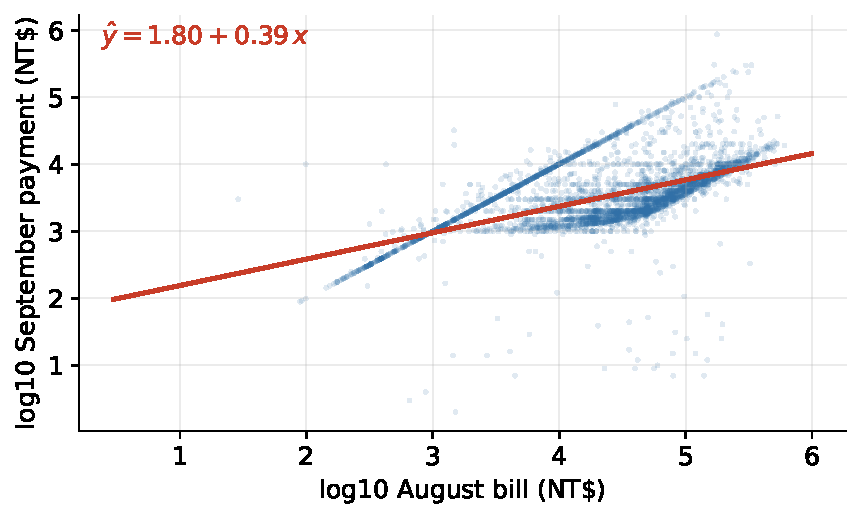
\includegraphics[width=0.56\textwidth]{lecture_2/figures/fig_linear_fit.pdf}
\caption{The warm-up fit: log payment on log bill. The slope is an
elasticity.}
\label{fig:linfit}
\end{figure}

Our warm-up (Figure~\ref{fig:linfit}) regresses log September payment on
log August bill among the 24{,}605 paying clients - Block 1's lens, put
to work. In a log-log specification the slope is an elasticity, and ours
reads 0.39: a 1\% larger bill draws only about 0.39\% more payment - the
revolvers absorb the rest, financing rather than repaying bill growth.
Quantifying the cloud's width introduces the three standard metrics:
$R^2$ (share of variance explained, unitless), RMSE and MAE (in the units
of the target - the language for business, with RMSE punishing large
misses and MAE robust to them). Our fit reaches $R^2 \approx 0.33$, and a
number like that is typical of behavioural targets: real relationships,
plenty of noise. The reverse deserves
the alarm: on behavioural data, a suspiciously high $R^2$ means leakage or
a target twin - investigate before celebrating.

\subsubsection{Log-log and elasticities: the algebra}
Why does a log-log slope read as ``percent per percent''? The algebra is
three lines and worth owning rather than trusting. Write the fitted
relationship as $\ln y = a + b \ln x$. Exponentiating, $y = A x^{b}$
with $A = e^{a}$ - the model is a power law in the original units. Now
perturb $x$ by a small fraction: differentiate to get
\[
  \frac{dy}{y} \;=\; b \, \frac{dx}{x},
\]
i.e.\ the \emph{relative} change in $y$ is $b$ times the \emph{relative}
change in $x$ - percent in, $b$ percent out, at any point on the curve.
That constancy is the whole appeal: in raw units the payment response to
a 1{,}000-unit bill increase depends on where you start, while in logs a
single number, the elasticity, summarises the response everywhere. For
our $b = 0.39$: a bill 1\% larger predicts a payment larger by the
factor $1.01^{0.39} \approx 1.0039$, i.e.\ about $0.39$\% - for small
changes the derivative version and the exact version agree to the
decimals shown. For large changes they do not: a bill \emph{doubling}
predicts payments scaling by $2^{0.39} \approx 1.31$, not by
$1 + 0.39 = 1.39$ - compound the elasticity, do not add it. And note
what $b < 1$ means economically before you ever check significance:
payments grow \emph{less} than proportionally with bills, so utilisation
drifts up as bills grow - the revolving mechanism, visible in one
exponent.

\begin{figure}[htbp]
\centering
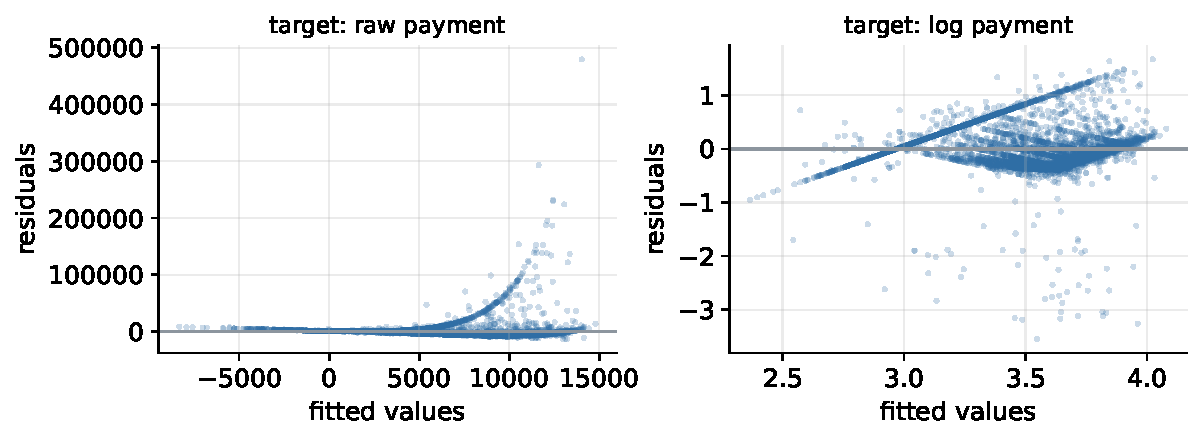
\includegraphics[width=0.86\textwidth]{lecture_2/figures/fig_residuals.pdf}
\caption{Residuals against fitted values, raw versus log target. The funnel
on the left is heteroscedasticity; the log transform fixes the model, not
just the histogram.}
\label{fig:resid}
\end{figure}

The diagnostic that tells the truth about any regression is the residual
plot (Figure~\ref{fig:resid}): residuals $y - \hat y$ against fitted
values, wanted structureless around zero. A funnel means error variance
grows with the prediction (heteroscedasticity) - the raw-payment fit has
exactly that, and the log target cures it. Curvature means missing
nonlinearity: engineer a feature.

\subsubsection{Reading residual plots like a professional}
Treat the residual plot as a small vocabulary and read it every time.
\emph{A structureless horizontal band}: the model has extracted what it
can; remaining scatter is (as far as this plot can see) honest noise.
\emph{A funnel opening rightward}: errors grow with the prediction -
multiplicative noise, the signature of monetary variables, and the
canonical cure is a log transform of the target, which turns
``errors proportional to size'' into ``errors constant in logs''. Note
what the cure means for prediction: if you model $\ln y$ and
exponentiate to report $\hat y$, your predictions are (roughly) medians,
not means, in the original units - fine for ranking, worth a footnote
when someone sums them into a portfolio total. \emph{A bow or curve}:
the conditional mean is not linear in your features - the model
systematically overpredicts in one range and underpredicts in another;
add a squared term, a log, or an interaction, guided by \emph{where} the
bow sits. \emph{Isolated extreme points}: outliers, and under squared
loss each one pulls with leverage proportional to its miss - revisit
Block 1's boxplots and decide, case by case, whether the point is an
error to fix or a customer to respect. What the residual plot cannot
show also matters: it is an in-sample diagnostic, so it certifies
specification, not generalisation - a leaky feature produces gorgeous
residuals and a useless model. The plot and the test score audit
different failures; you need both.

\subsubsection{$R^2$ and its failure modes}
$R^2$ is the most quoted and most misread number in regression, so we
give its pathologies their own paragraph. \emph{Failure mode one:
in-sample monotonicity.} By the projection argument, adding any column -
a noise column, an astrology column - never lowers in-sample $R^2$. A
model with enough junk features can push in-sample $R^2$ wherever you
like; the adjusted $\bar R^2$ patches this with a parameter penalty, but
the honest fix is the one this chapter keeps prescribing: compute $R^2$
\emph{out of sample}, on the test set, where junk features hurt rather
than help. \emph{Failure mode two: the sign.} Out-of-sample $R^2$
compares your model's squared error against predicting a constant mean -
and your model can lose. Out-of-sample $R^2$ below zero is not a bug in
the library; it is the report that your model generalises worse than a
horizontal line, which overfit models regularly do. \emph{Failure mode
three: no intercept.} The usual variance decomposition behind $R^2$
requires the residuals to sum to zero, which the intercept guarantees;
fit through the origin and software packages fall back on different
formulas, producing $R^2$ values that are not comparable to anything -
if you must drop the intercept, stop quoting $R^2$. \emph{Failure mode
four: across transforms.} An $R^2$ on $\ln y$ and an $R^2$ on $y$
measure explained variance of \emph{different targets}; our 0.33 on log
payments cannot be compared with a raw-payment fit's number, and neither
is ``the'' $R^2$ of the problem. \emph{Failure mode five: the silent
range restriction.} $R^2$ is relative to the target variance in the
sample at hand; score the same model on a narrower subpopulation and
$R^2$ drops with no change in the model's error - which is also why
$R^2$ quoted on extrapolated predictions, outside the training range,
is fiction twice over. None of this makes $R^2$ useless; it makes it a
single, context-bound summary - quote it out of sample, alongside RMSE
in business units, and never alone.

Reading coefficients without embarrassment takes three habits. First,
units: $\beta_j$ is the change in $y$ per one unit of $x_j$ - per NT\$,
per thousand, per SD? Standardising features (mean 0, SD 1) makes
coefficients comparable as effects-per-SD. Second, remember coefficients
are teammates, not soloists: adding or removing a correlated feature
reshuffles the others, and Block 1's correlation map says which ones.
Third, ``holding others fixed'' is a statistical statement, not a causal
one - the Simpson's-paradox caution applies to coefficients too.

Categorical features enter via one-hot encoding with one level dropped as
the \emph{reference}: keeping all levels alongside an intercept creates
perfect collinearity (the dummy variable trap). Each dummy coefficient then
reads ``versus the reference'', so choose the reference deliberately -
it changes the story, not the fit. More generally, when two features carry
near-identical information, least squares cannot decide how to split the
credit between them: coefficients take absurd signs and sizes and swing
between samples while predictions stay fine - \emph{prediction survives,
interpretation dies}. Remedies: drop one twin, combine them (a ratio), or
regularise. The diagnostic keyword is the variance inflation factor (VIF).

\subsubsection{Multicollinearity and the VIF, quantified}
The VIF deserves the two minutes it takes to demystify. For feature
$j$, regress $x_j$ on all the \emph{other} features and record the
$R_j^2$ of that auxiliary regression - how predictable this feature is
from its colleagues. Then
\[
  \mathrm{VIF}_j \;=\; \frac{1}{1 - R_j^2},
\]
and the sampling variance of $\hat\beta_j$ is inflated by exactly this
factor relative to the uncorrelated-features ideal. The arithmetic makes
the folklore thresholds concrete: $R_j^2 = 0.5$ gives VIF $2$ - mild;
$R_j^2 = 0.9$ gives VIF $10$ - the classic alarm level, at which the
standard error of $\hat\beta_j$ is $\sqrt{10} \approx 3.2$ times larger
than it would otherwise be; $R_j^2 = 0.99$, the near-duplicate case,
gives VIF $100$ and coefficients that are pure noise. Notice what the
formula does \emph{not} contain: the target. Multicollinearity is a
property of the feature matrix alone, which is why it damages the
decomposition (coefficients) and not the projection (predictions) - the
geometric asymmetry from the projection picture, now with a number
attached. Practical protocol for credit work: compute VIFs on the final
feature set; for any feature above 10, decide openly - drop a twin,
build the ratio (utilisation \emph{is} such a repair: bill and limit,
individually collinear with everything, combined into one interpretable
feature), or accept the inflated coefficient and refrain from
interpreting it. What is not acceptable is interpreting a VIF-10
coefficient's sign in front of a risk committee as if it were stable.

A last piece of linear-model vocabulary: \emph{interactions}. In the plain
additive model, utilisation contributes the same slope for every customer.
If in reality utilisation bites harder after payment delays, the model
needs a product column:
\[
  y = \beta_0 + \beta_1\,\text{util} + \beta_2\,\text{delayed}
      + \beta_3\,(\text{util}\times\text{delayed}),
\]
after which the utilisation slope becomes $\beta_1 + \beta_3\,
\text{delayed}$ - one feature \emph{moderates} another
(Figure~\ref{fig:interactions2}). Without the interaction term the two
groups get parallel lines (shifted intercepts, one slope); with it, the
slopes may differ. Two lessons attach. First, a linear model cannot
discover an interaction on its own: the product column is feature
engineering - Block 1's interaction move, graduated into a term, and one more place where domain knowledge enters the model by hand.
Second, this is a genuine limitation of linear models that tree-based
models do not share: trees carve the feature space region by region and
pick up interactions automatically, which is one of the reasons they win on
tabular data (Block 3). In logistic regression the same construction works
on the log-odds scale, and the interaction coefficient exponentiates into a
\emph{ratio of odds ratios} - interpretable, but read it slowly.

\begin{figure}[htbp]
\centering
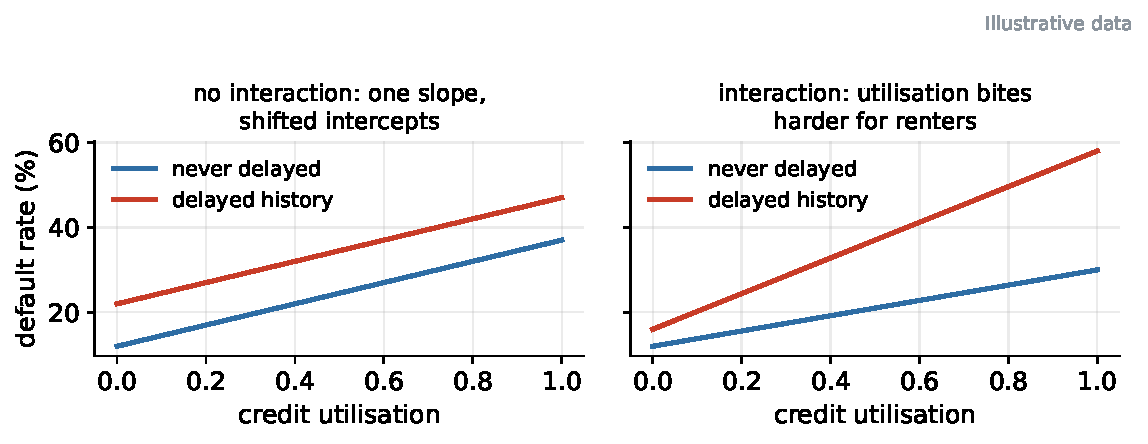
\includegraphics[width=0.74\textwidth]{lecture_2/figures/fig_interactions.pdf}
\caption{Additive effects give parallel lines; an interaction lets one
feature change another's slope (illustrative data).}
\label{fig:interactions2}
\end{figure}

\subsection{Logistic regression: the credit-scoring workhorse}
Fit a straight line to a 0/1 target and it breaks visibly
(Figure~\ref{fig:lpm}): predictions escape $[0,1]$, producing ``$-7$\%''
and ``130\%'' probabilities. The repair keeps the linear machinery
$z = \beta_0 + \beta_1 x_1 + \dots$ and squashes it through the sigmoid
$\sigma(z) = 1/(1+e^{-z})$, which maps any score to a probability.

\subsubsection{The linear probability model: broken, but not worthless}
Before discarding the straight line, give it its due, because your
econometrics courses did not teach it to you by accident. Fitting OLS to
a 0/1 target is called the \emph{linear probability model} (LPM), and
its defects are structural, not cosmetic. The escaping predictions you
saw are one; a second is baked into the target itself: a 0/1 outcome
with success probability $p(x)$ has conditional variance $p(x)(1-p(x))$,
which \emph{changes with} $x$ - the LPM is heteroscedastic by
construction, no residual plot needed to suspect it. A third is the
constant-slope assumption: the LPM insists that one more month of delay
adds the same probability increment to a pristine customer as to one
already at the cliff edge, which contradicts everything the sigmoid's
shape (and common sense) says about saturation near 0 and 1. Yet the LPM
survives in econometric practice for a defensible reason: its
coefficients \emph{are} marginal effects on the probability scale,
directly, with no transformation - a convenience causal researchers
prize, and with everyone's probabilities sitting in a moderate middle
range the linear and logistic fits barely differ. The division of
labour, then: for estimating an average treatment effect, the LPM is a
legitimate tool; for producing per-customer PDs that must live in
$[0,1]$, feed a pricing engine, and extrapolate sanely into the tails -
our job - it is the wrong tool, and the sigmoid is the repair.

\begin{figure}[htbp]
\centering
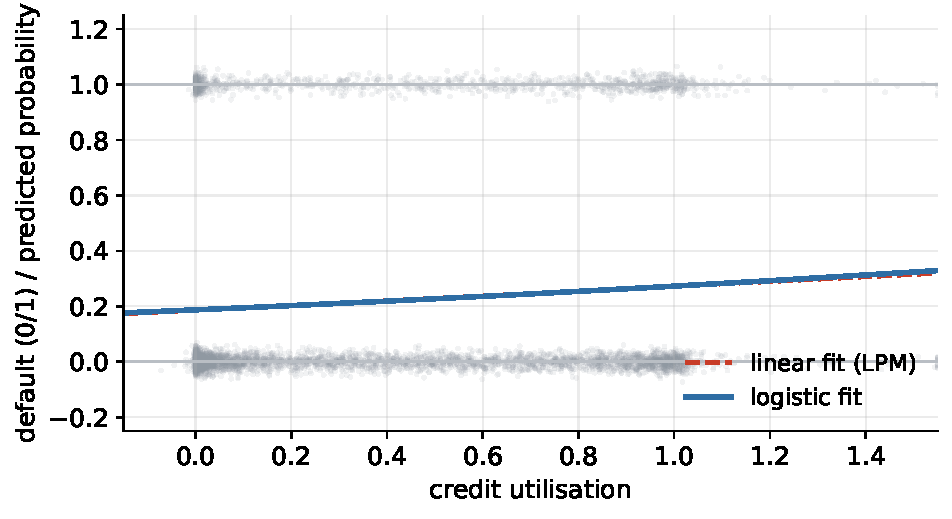
\includegraphics[width=0.6\textwidth]{lecture_2/figures/fig_lpm_vs_logistic.pdf}
\caption{A linear fit to the 0/1 default indicator leaves $[0,1]$; the
logistic curve lives there natively.}
\label{fig:lpm}
\end{figure}

The natural scale of the model is odds. With
$\text{odds} = p/(1-p)$, the model says
\[
  \ln\frac{p}{1-p} \;=\; \beta_0 + \beta_1 x_1 + \dots + \beta_k x_k ,
\]
i.e.\ logistic regression is \emph{linear in log-odds} - that is the
sense in which it is a linear model. ($p = 0.5$ is odds $1{:}1$ and
log-odds $0$; $p = 0.9$ is odds $9{:}1$ and log-odds $+2.2$.) Fitting
replaces least squares with maximum likelihood: minimise the log-loss
\[
  -\frac{1}{n}\sum_{i=1}^{n}\bigl[\,y_i \ln \hat p_i +
  (1-y_i)\ln(1-\hat p_i)\bigr],
\]
which punishes confident wrongness brutally ($\hat p = 0.99$ for a customer
who repays costs $-\ln 0.01 \approx 4.6$; a humble $0.6$ costs $0.9$).
There is no closed form; sklearn iterates silently, and the same loss
reappears inside neural networks in Block 6.

\subsubsection{Logistic regression as a GLM, and one line of calculus}
For the statistically minded, the tidy frame is the \emph{generalised
linear model}: keep a linear predictor $z = \beta_0 + \sum_j \beta_j
x_j$, choose a distribution for the target (here Bernoulli), and connect
the two with a \emph{link function} - here the logit,
$\ln\bigl(p/(1-p)\bigr) = z$, whose inverse is the sigmoid. Linear
regression is the same skeleton with a Gaussian target and the identity
link; Poisson regression for counts is a third sibling. Seeing the
family matters beyond taxonomy: it says the modelling choice is really
two choices - what noise the target carries, and on what scale effects
are additive - and logistic regression answers ``Bernoulli'' and ``the
log-odds scale''. The fitting story also collapses to one satisfying
line of calculus. The sigmoid differentiates into itself:
$\sigma'(z) = \sigma(z)\,(1 - \sigma(z))$. Chain that through the
log-loss of one observation and everything cancels except
\[
  \frac{\partial \, \text{loss}_i}{\partial \beta_j}
  \;=\; (\hat p_i - y_i)\, x_{ij},
\]
the prediction error times the feature - the exact same shape as the
OLS gradient, with $\hat p$ in place of $\hat y$. The consequences are
worth collecting. At the optimum the errors $(\hat p_i - y_i)$ are
orthogonal to every feature, the projection intuition reborn on the
log-odds scale; with an intercept in the model the average predicted
probability exactly equals the observed default rate, a free
calibration-in-the-large check; and because the log-loss is convex in
$\beta$, the iterative fit finds \emph{the} optimum, not \emph{an}
optimum - part of why logistic regression is so reproducibly stable.
Block 6's neural networks will use this identical gradient, stacked
deeper; the derivative you just read is the last layer of every
classification network you will ever train.

\begin{figure}[htbp]
\centering
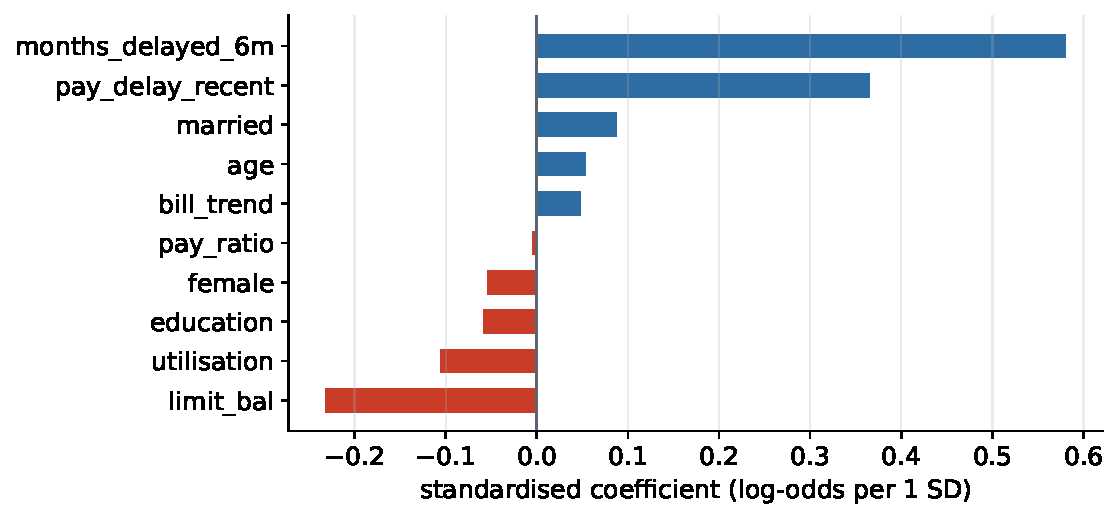
\includegraphics[width=0.62\textwidth]{lecture_2/figures/fig_logit_coefs.pdf}
\caption{Standardised coefficients of the PD baseline. The strongest
feature in the model is Block 1's craft at work: the engineered delay
counter \texttt{months\_delayed\_6m}.}
\label{fig:coefs}
\end{figure}

Fitted to the real portfolio (standardised features, leakage-safe
pipeline), the baseline's coefficients read like a page of credit wisdom
(Figure~\ref{fig:coefs}). Payment history is king: the engineered delay
counter \texttt{months\_delayed\_6m} ($+0.58$) and the most recent
repayment status ($+0.37$) tower over everything - Block 1's
feature-engineering craft vindicated on real data. And one haunting:
\texttt{limit\_bal} enters at $-0.23$ - higher limits, \emph{lower} risk
- because the bank's historical screening granted large limits to safe
clients. That is Block 1's selection bias, visible inside a coefficient.
Exponentiating turns coefficients into odds multipliers:
$e^{\beta_j\Delta}$ scales the odds per $\Delta$ of $x_j$. One SD more
months-delayed multiplies the odds of default by $e^{0.58} \approx 1.8$;
one SD more limit multiplies them by $e^{-0.23} \approx 0.79$. Effects
compound multiplicatively: two $\times 1.8$ moves make $\approx
3.2\times$, not ``$+2\times$something''.

Pause on the \texttt{limit\_bal} coefficient once more, because it is
this chapter's cleanest specimen of the inference-prediction divide made
flesh. Causally, the sign is backwards: handing a risky customer a
larger limit does not make them safer - the arrow runs the other way,
from the bank's past risk assessment to the limit. An econometrician
must treat this coefficient as an endogeneity problem to be
instrumented away. A predictor may keep it: at scoring time the granted
limit genuinely carries information about the customer (it summarises a
previous underwriter's file review), and the model is right to use it -
as long as nobody reads it as advice to raise limits, and as long as
everyone notices the dependency it creates: if the bank's granting
policy changes, this coefficient's usefulness quietly expires. One
coefficient, three lessons: prediction can use what causation cannot
bless, every predictive model borrows against the stability of the
process that generated its data, and the sign of a coefficient is a
question, never an answer.

Interpretation becomes concrete at the level of a single customer.
Because the model is linear in log-odds, every prediction decomposes
exactly: each feature contributes $\beta_j x_j$ (standardised units), the
contributions plus the intercept sum to $z$, and $\sigma(z)$ is the PD.
Figure~\ref{fig:contrib} shows the receipt for one test customer: recent
delays push the log-odds up, a high limit pulls them down, and the pieces total $z = 0.62$, i.e.\
a PD of 65\%. Two things follow. Practically, adverse-action reasons fall
straight out of the largest positive bars - the explanation \emph{is}
the model. Methodologically, this exact, free decomposition is the object
that SHAP (Block 3) approximates for models that are not this polite;
students who understand this figure already understand what a SHAP plot
is trying to be.

\begin{figure}[htbp]
\centering
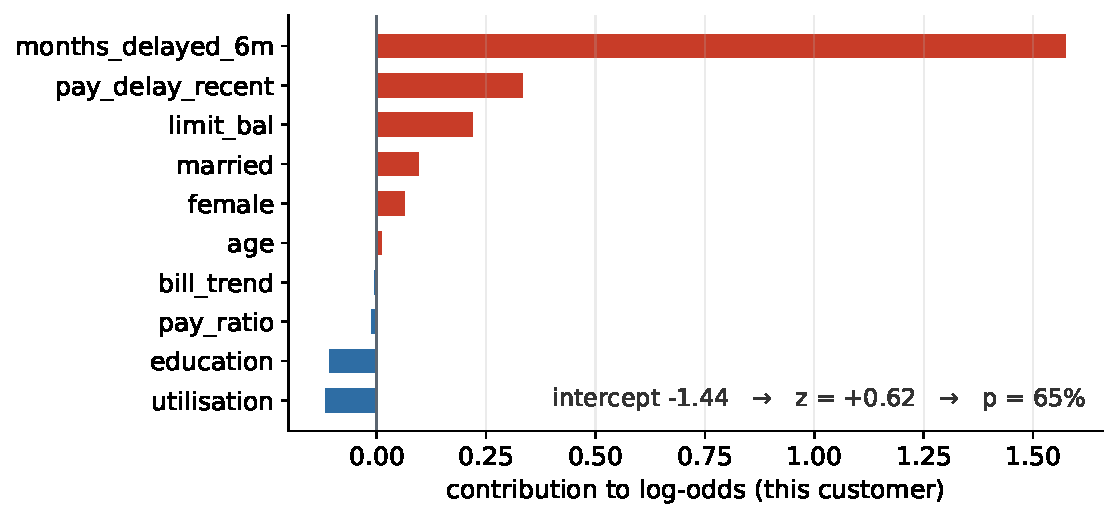
\includegraphics[width=0.62\textwidth]{lecture_2/figures/fig_customer_contrib.pdf}
\caption{One customer's prediction, decomposed into exact per-feature
log-odds contributions.}
\label{fig:contrib}
\end{figure}

One subtlety separates competent readings from embarrassing ones: odds
ratios are constant, probability effects are not. The same
$\times 1.54$ odds multiplier moves a 10\% PD to 14.6\% ($+4.6$ pp), a
50\% PD to 60.6\% ($+10.6$ pp), and a 90\% PD to 93.3\% ($+3.3$ pp) -
the sigmoid is steep in the middle and flat in the tails, with marginal
effect $\partial p/\partial x_j = \beta_j\, p(1-p)$, maximal at
$p = 0.5$. When communicating, always say which scale you are on, and
report probability changes in \emph{percentage points}: ``risk rose 10
percent'' and ``risk rose 10 percentage points'' are claims an order of
magnitude apart, and mixing them up in a risk committee is not soon
forgotten.

\subsubsection{Odds ratios versus marginal effects, with the arithmetic}
Let us make the two dialects fully concrete, because committee
conversations switch between them mid-sentence and you must not get
lost. Take the $\times 1.54$ odds multiplier ($\beta = 0.43$ per SD of
utilisation) and trace the 10\% customer by hand. Odds before:
$0.10/0.90 = 1/9 \approx 0.111$. Odds after: $0.111 \times 1.54 \approx
0.171$. Probability after: $0.171/(1 + 0.171) \approx 0.146$ - the
14.6\% in the table, no magic, three lines of arithmetic you can
reproduce on a napkin. The derivative shortcut answers the same question
locally: at a PD near our portfolio's 22\% base rate, the marginal
effect is $\beta\, p(1-p) \approx 0.43 \times 0.22 \times 0.78 \approx
0.074$ - roughly $7$ percentage points of PD per SD of utilisation, for
customers near the base rate. The same $\beta$, applied at $p = 0.05$,
yields $0.43 \times 0.05 \times 0.95 \approx 0.020$ - just $2$ points,
because the sigmoid is flat down there. Hence the reporting rules of the
trade. The odds ratio is the \emph{model's} native constant - one
number, true everywhere, but in a currency (odds) most audiences only
think they understand. The marginal effect is the \emph{audience's}
currency - percentage points - but it is local: it depends on the
customer's starting PD, so you must state where it was evaluated
(``at the base rate'' being the usual convention, averaged-over-sample
effects the more careful one). Reporting a single probability effect as
if it applied to everyone is the most common quantitative error in
model documentation; you are now inoculated.

\subsubsection{The scorecard tradition: WoE, points, and why banks still care}
The scorecard is not nostalgia; it is a parallel formulation of exactly
the model you just fitted, engineered for governance, and its logic
rewards a closer look. The classical stack has three moves. First,
\emph{bin} each feature into a handful of intervals (utilisation into,
say, five bands) - deliberately coarse, which throws away wiggle-room
and thereby regularises (the leash principle of
Section~\ref{sec:regularisation}, avant la lettre). Second, replace each
bin with its \emph{weight of evidence}: the log of the ratio between the
share of good customers and the share of bad customers landing in the
bin. WoE is a log-odds-shaped encoding, so a logistic regression on WoE
features is linear on the same scale twice over - the construction makes
the model \emph{additive in bins}, each bin carrying an evidential
weight with a sign anyone can audit (negative WoE bin: this range of
values is bad news). Third, rescale log-odds into \emph{points}: choose
a base score and a points-to-double-the-odds constant (20 is customary),
and the score is an affine function of the same $z$ - with $20$ points
per doubling, each point multiplies the odds by $2^{1/20} \approx
1.035$. The result is a table a branch officer can apply with a pencil
and a validator can check line by line: this bin, these points, summed,
compared to a cut-off. Every property regulators like - monotone bins,
visible contributions, no customer scored outside the table's range -
was bought by discarding flexibility a GBDT would have kept, which is
the whole trade stated honestly: scorecards sit deliberately left of the
U-curve's bottom, paying a little accuracy for a lot of accountability.

\begin{practice}
A credit score is a rescaled log-odds: choose a base score and a
``points to double the odds'' constant, and the scorecard is linear in the
same $z$ the model computes. The classical stack - logistic regression on
WoE-encoded bins, formatted as a scorecard - has run production lending
for decades because each feature's contribution is a number an auditor can
read line by line. Modern practice often runs GBDT for power and a
scorecard for explainability, side by side.
\end{practice}

Prediction needs one more step: a decision. The predicted-probability
distributions of the two classes overlap
(Figure~\ref{fig:probhist}) - no threshold separates them cleanly, and
0.5 is not a law of nature but a library default. Which threshold to use is
a cost question, taken up in Section~\ref{sec:eval1}. Three honest notes on
imbalance complete the picture: real PD portfolios (1--5\% default rates)
push predicted probabilities so low that a 0.5-threshold model may never
predict ``default'' - a threshold problem, not a model problem;
\texttt{class\_weight="balanced"} re-weights the loss but distorts
predicted probabilities, so recalibrate if probabilities matter (in
pricing, they do); and resampling schemes are popular and overrated -
try thresholds and weights first.

\begin{figure}[htbp]
\centering
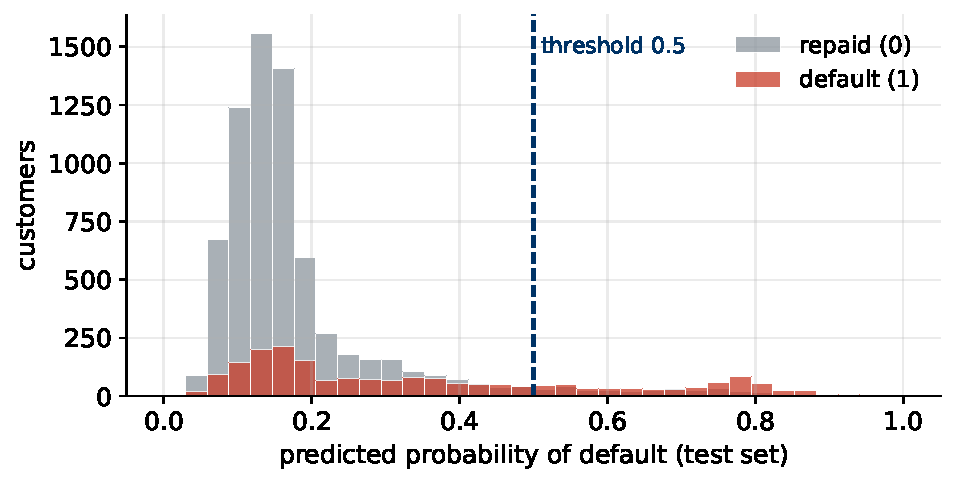
\includegraphics[width=0.62\textwidth]{lecture_2/figures/fig_pred_prob_hist.pdf}
\caption{Predicted default probabilities by true class, test set. The
overlap is why thresholds are decisions, not constants.}
\label{fig:probhist}
\end{figure}

Why crown logistic regression \emph{the} baseline? It is fast
(milliseconds, millions of rows), stable (decent with zero tuning),
explainable (coefficients $\to$ odds ratios $\to$ adverse-action reasons),
and an honest yardstick. The baseline discipline of this course: no GBDT,
no neural network, no ensemble gets built - in class or in projects -
before a logistic baseline exists for it to beat. The discipline has a
quiet second payoff: the baseline is a \emph{measuring instrument} for
your features. Because logistic regression can only use what you hand it
- no automatic interactions, no carved regions - its performance is a
direct read on feature quality, and the gap between it and a later GBDT
is a direct read on how much nonlinearity and interaction structure your
problem actually contains. A small gap says the signal was linear all
along and the complex model is decoration; a large gap says go hunting
for the interactions the trees found and consider engineering them into
the scorecard. Either way you learn something no single model run could
tell you - which is the deeper reason baselines are non-negotiable.

\subsection{Regularisation}
\label{sec:regularisation}
Many features, correlated features and finite data conspire to tailor
coefficients to this sample's noise - the U-curve wearing a suit. The
cure is to charge for coefficient size: add a penalty to the loss, so the
model must buy each unit of coefficient with genuine predictive payoff. A
little bias in, a lot of variance out - usually a bargain on test error.

\subsubsection{The mechanics, in one small example}
To see shrinkage operate rather than just hear it described, take the
smallest possible case: one standardised feature, so OLS gives some
slope $\hat\beta$. Ridge with penalty $\alpha$ replaces it with
\[
  \hat\beta_{\text{ridge}}
  \;=\; \hat\beta \cdot \frac{S}{S + \alpha},
\]
where $S$ is the feature's (scaled) sum of squares - a pure shrinkage
factor between 0 and 1. With $S = 100$ and $\alpha = 25$, every unit of
OLS slope survives at 80\%; crank $\alpha$ to 400 and only 20\%
survives; at $\alpha = 0$ you have OLS back, and as $\alpha \to \infty$
the coefficient - and the model's variance with it - goes to zero,
leaving the intercept: maximal bias, zero variance. The dial between
those endpoints \emph{is} the U-curve's steering wheel, now with a
formula on it. The multi-feature version keeps the moral and adds a
subtlety: ridge shrinks hardest in the directions where the data is
thinnest - exactly the ambiguous, nearly-parallel directions that
multicollinearity leaves ill-determined - and barely touches directions
the data pins down well. That is why ridge is the multicollinearity
remedy: it does not pick a winner between twin features, it splits the
coefficient between them and stabilises both. Lasso's absolute-value
penalty changes the character of the solution rather than just its
size, as the paths and the geometry below show.

\begin{figure}[htbp]
\centering
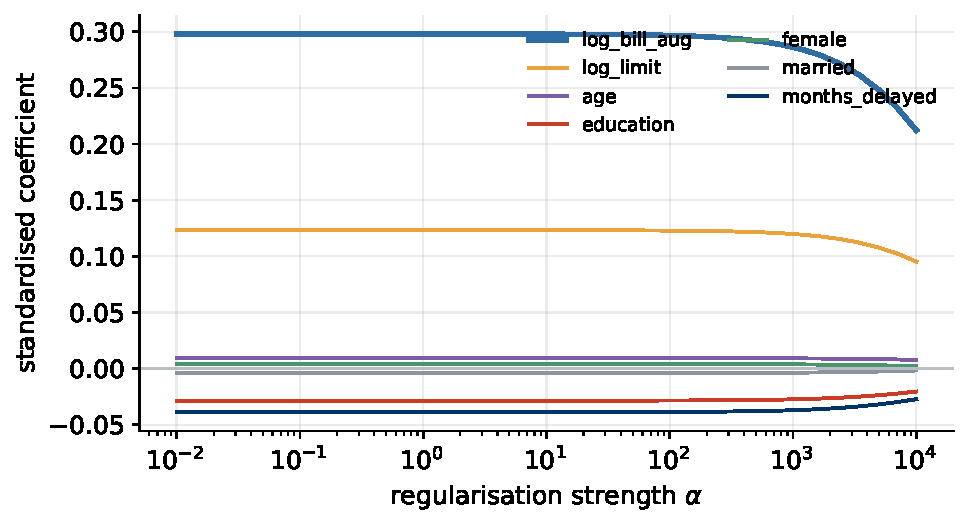
\includegraphics[width=0.6\textwidth]{lecture_2/figures/fig_ridge_paths.pdf}
\caption{Ridge coefficient paths: smooth shrinkage, never exactly zero.}
\label{fig:ridge}
\end{figure}

\begin{figure}[htbp]
\centering
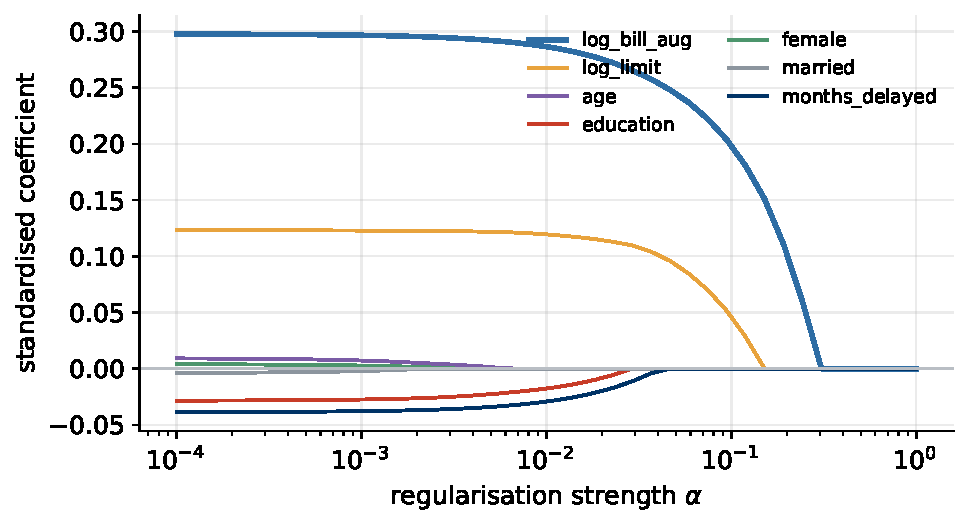
\includegraphics[width=0.6\textwidth]{lecture_2/figures/fig_lasso_paths.pdf}
\caption{Lasso coefficient paths: features leave the model one by one.
Note the $\alpha$ scale - L1 bites at much smaller $\alpha$ than ridge.}
\label{fig:lasso}
\end{figure}

Two classic penalties, two personalities. \textbf{Ridge} (L2) adds
$\alpha \sum_j \beta_j^2$: as $\alpha$ grows every coefficient shrinks
smoothly toward zero without reaching it
(Figure~\ref{fig:ridge}), and correlated twins share the credit - the
multicollinearity remedy. \textbf{Lasso} (L1) adds
$\alpha \sum_j |\beta_j|$: coefficients hit exactly zero one by one
(Figure~\ref{fig:lasso}), giving built-in feature selection - though with
twins it keeps one and drops the other, a choice not to be read causally.
The geometry explains the guillotine
(Figure~\ref{fig:geometry}): the penalised solution is the first touch
between the equal-loss ellipses around the OLS optimum and the
coefficient-budget region; a circle can be touched anywhere, so ridge
coefficients get small but stay nonzero, while a diamond gets hit at its
corners - and corners have $\beta_j = 0$ exactly. \textbf{Elastic net}
mixes the two; when in doubt, mix.

The corner argument rewards a slow second reading, because it explains a
fact that otherwise looks like luck. Picture the two-coefficient plane.
Around the unpenalised optimum sit ellipses of equal training loss;
around the origin sits the budget region - a disc for L2 (fixed
$\beta_1^2 + \beta_2^2$), a diamond for L1 (fixed
$|\beta_1| + |\beta_2|$). The penalised solution is where a growing
ellipse first grazes the budget. A disc's boundary is smooth: the first
touch can land anywhere on it, and landing exactly where a coordinate is
zero is a measure-zero coincidence - so ridge coefficients get small
but essentially never vanish. A diamond, though, has corners, and the
corners sit \emph{on the axes} - points where one coefficient is
exactly zero - and a corner, being pointy, presents itself to the
approaching ellipse from many angles at once: a whole range of ellipse
orientations all hit the same corner first. Sparsity is thus not a
numerical accident of L1 but a geometric attractor: the corner
\emph{catches} solutions. In higher dimensions the diamond's corners and
edges are entire regions with many coefficients at zero, and the catch
gets stronger - which is why lasso on a wide feature matrix confidently
returns a short list.

\begin{figure}[htbp]
\centering
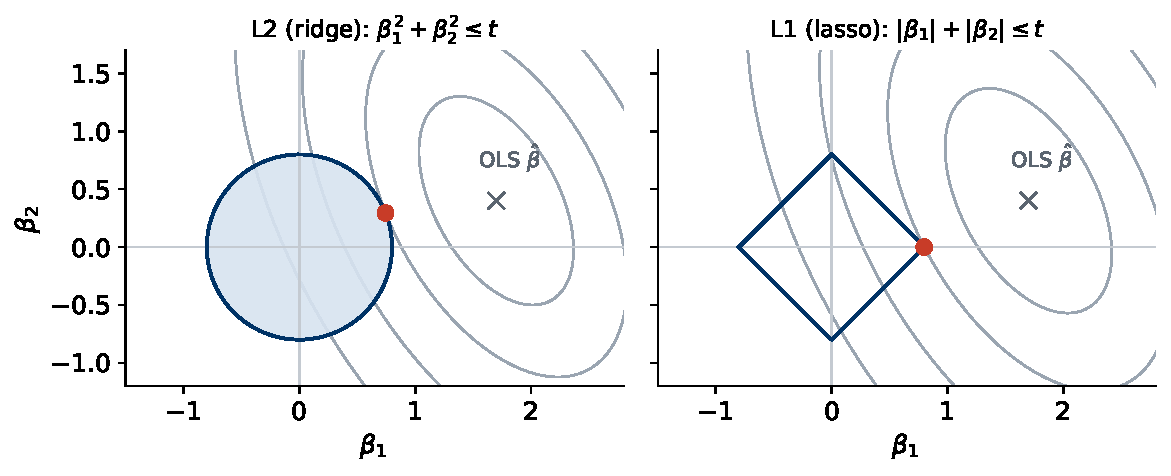
\includegraphics[width=0.7\textwidth]{lecture_2/figures/fig_l1_l2_geometry.pdf}
\caption{Why lasso zeros coefficients: loss contours meet the L2 disc
anywhere, but meet the L1 diamond at a corner.}
\label{fig:geometry}
\end{figure}

Two operational rules make penalties meaningful. \emph{Scale first}: the
penalty charges by coefficient size, and size depends on units -
unscaled, it punishes features for their units rather than their
usefulness; standardise before any penalised model, fitting the scaler on
the training data only (the Block 1 golden rule again - and sklearn will
not warn you). To feel why this rule is mandatory rather than tidy,
run the units experiment in your head: express the credit limit in
single currency units and its coefficient is numerically tiny (a huge
number multiplies it); express age in years and its coefficient is
numerically large. The penalty, blind to units, taxes the age
coefficient heavily and the limit coefficient not at all - it has
silently decided that limits matter and age does not, based on nothing
but bookkeeping. Rescale the limit into thousands and the ``importance''
reverses. A penalised model on unscaled features is not a worse model;
it is an arbitrary one. \emph{Choose $\alpha$ on validation data}:
$\alpha$ is a
hyperparameter, so the data that fit the coefficients cannot also pick it.
Figure~\ref{fig:valcurve} shows the sweep on a deliberately high-variance
version of our payments-from-bills problem (80 training rows, polynomially expanded
features): training error rises monotonically with $\alpha$ while
validation error traces a genuine U with an interior optimum
($\alpha \approx 50$). Done properly - with cross-validation - next
week. Read the two curves of Figure~\ref{fig:valcurve} as the
bias-variance ledger in motion: at tiny $\alpha$ the model is nearly
unpenalised, training error is flattering and validation error pays the
variance bill; at huge $\alpha$ everything is shrunk toward zero and
both curves meet in shared, biased mediocrity; the interior minimum is
where the last unit of variance removed stopped being worth the bias it
cost. Every hyperparameter sweep you run in this course - tree depth
next week, learning rate in Block 6 - will produce this same pair of
curves, and you will read them the same way.

\begin{figure}[htbp]
\centering
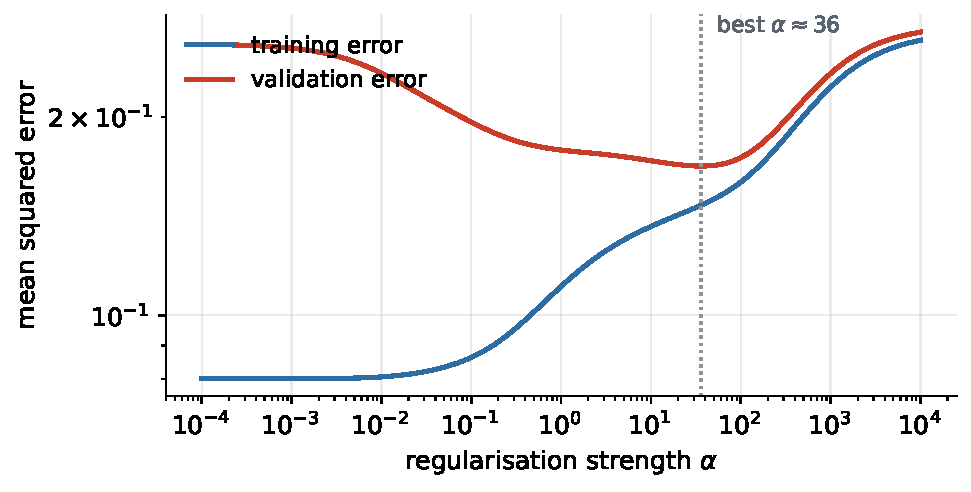
\includegraphics[width=0.6\textwidth]{lecture_2/figures/fig_validation_curve.pdf}
\caption{Choosing $\alpha$: the validation curve on a high-variance setup.}
\label{fig:valcurve}
\end{figure}

\begin{practice}
In \texttt{LogisticRegression} the knob is \texttt{C} $= 1/\alpha$ -
\emph{bigger} C means \emph{weaker} penalty - and regularisation is on by
default (\texttt{C=1}). Everyone who has ever fitted sklearn's logistic
regression has been regularising, mostly without knowing. Also remember
what penalties cannot do: they control coefficients, not data quality, and
will happily shrink their way around leakage without curing it.
\end{practice}

Penalties are one instance of a universal idea: put a leash on flexibility
and generalisation improves. Max depth and minimum leaf size leash trees
(Block 3); learning rate and the number of rounds leash GBDT (Block 3);
early stopping and dropout leash neural networks (Block 6); even WoE's
coarse bins leash scorecards. Different mechanics, one U-curve - so when
you meet a new model family, your first question is fixed: \emph{where is
its leash?} The implementation partner of all of this is the sklearn
\texttt{Pipeline}, which welds preprocessing to the model so that whatever
data the model sees, its transforms were fitted on the corresponding
training part - not style advice, but the only way to stay leakage-free
inside cross-validation.

\subsection{Feature selection}
Regularisation shrinks coefficients; \emph{feature selection} removes
columns outright. The two overlap (lasso is both) but selection deserves
its own frame, because in credit work the pressure to shorten the feature
list comes from everywhere at once: regulators want auditable inputs,
engineers want cheap pipelines, and Block 4's curse of dimensionality
wants fewer voters. The standard taxonomy has three families.

\textbf{Filter methods} score each feature against the target before any
model is fitted: correlations (point-biserial for a binary target),
mutual information, and credit scoring's own \emph{Information Value}
computed from WoE bins, with the folklore bands (IV $<$ 0.02 useless,
0.1-0.3 medium, $>$ 0.5 suspicious - the last band being a leakage
smell, not a triumph). The IV construction is worth one sentence beyond
the folklore: it sums, over a feature's bins, the difference between the
good and bad distribution shares weighted by the bin's WoE - so a
feature scores high exactly when its bins separate the two populations,
and the ``$> 0.5$ is suspicious'' band encodes hard-won experience that
honest application-time features rarely separate good from bad
\emph{that} well; the ones that do usually contain a whiff of the
outcome. Filters are fast and blind: they see each feature
alone, so they keep redundant twins and miss features that only work in
combination (Block 2's interaction lesson in reverse).

\textbf{Wrapper methods} search over feature subsets using the model
itself as the judge - forward selection adds the best next feature,
backward elimination drops the least missed one, recursive feature
elimination (RFE) automates the loop. Wrappers see combinations but cost
many model fits and, run carelessly, overfit the validation data - the
multiple-testing warning of Block 5 applies to feature search too.

\textbf{Embedded methods} let the model choose while training: lasso
zeroes coefficients (Block 2), and tree ensembles supply importance
rankings (Block 3) that can gate a shortlist. Embedded selection
inherits the model's biases - impurity importance's fondness for
high-cardinality features among them.

Two rules keep any of the three honest. First, selection is a fitted
transform: it must happen \emph{inside} the pipeline, on training data
only - selecting features on the full dataset and then cross-validating
is one of the classic leakage recipes (features were chosen while
peeking at every fold's test rows). Second, report stability: rerun the
selection across folds or bootstrap samples and publish how often each
feature survives; a feature that appears in half the reruns is a
coin-flip, not a finding. On our ten-feature Taiwan matrix selection is
cosmetic; on a 300-variable bureau feed it is a week of the project and
the difference between a model validation passes and one it does not.

\subsection{Evaluating classifiers, part 1}
\label{sec:eval1}
Our PD baseline scores 80.6\% accuracy on the held-out test set of
9{,}000 real clients. A model that always predicts ``repaid'' scores
77.9\%. Three
points better than doing nothing - is the model useless? No: it ranks
customers well, but accuracy at an arbitrary threshold cannot see that.
Diagnosis requires opening the box of ``right and wrong'':

\begin{center}\small
\begin{tabular}{@{}ll|cc@{}}
\toprule
 & & \multicolumn{2}{c}{Predicted} \\
 & & default & repaid \\
\midrule
\multirow{2}{*}{Actual}
 & default & TP $= 541$ (caught) & FN $= 1{,}450$ (missed) \\
 & repaid & FP $= 294$ (falsely declined) & TN $= 6{,}715$ (rightly approved) \\
\bottomrule
\end{tabular}
\end{center}

Four numbers, four different business events. At threshold 0.5 our
baseline is cautious: it raises few false alarms (294) and misses
1{,}450 of 1{,}991 defaulters. Whether that is good depends on prices: a false negative
costs roughly the \emph{principal}; a false positive costs the
\emph{margin} plus possibly the customer - amounts an order of magnitude
apart, with the ratio belonging to the business, not the data scientist.

\subsubsection{The accuracy trap, with the arithmetic laid bare}
The trap's mechanism is arithmetic, so run the arithmetic. Accuracy is
correct predictions over all predictions - and under imbalance the
majority class supplies almost all of both. Our 77.9\% do-nothing score
is just the complement of the 22.1\% base rate: predict ``repaid'' for
everyone and you are automatically right for every one of the repaying
majority. Push the imbalance to a realistic loan book at a 2\% default
rate and the do-nothing model scores 98\% - a number that would earn
applause at a board meeting while describing a model that has literally
never flagged a single risk. The general lesson: accuracy's baseline is
not 50\%, it is the majority share, so an accuracy figure is
uninterpretable until placed next to the base rate - and the gap
between them, not the level, is the model's contribution. There is a
second, subtler jaw to the trap: accuracy weighs both error types
equally, at one point each, while our two errors differ in cost by an
order of magnitude. A metric that prices a missed defaulter equal to an
unnecessarily declined customer is optimising a bank that does not
exist. Both jaws close at once on threshold-0.5 classifiers under
imbalance, which is why ``what is the model's accuracy?'' is, for PD
work, a question that mostly reveals who has not yet taken this course.

\subsubsection{Confusion-matrix economics: pricing the cells}
The confusion matrix stops being a table and starts being a business
report the moment you attach prices, so let us do it once with
illustrative round numbers - say a missed defaulter (FN) costs
10{,}000 in lost principal and a falsely declined good customer (FP)
costs 1{,}000 in lost margin, a deliberately crude 10:1 ratio of the
right order. Price our matrix at threshold 0.5: $1{,}450 \times 10{,}000
+ 294 \times 1{,}000 = 14.79$M of error cost. Now price two do-nothing
strategies. Approve everyone: $1{,}991 \times 10{,}000 = 19.9$M. Decline
everyone: $7{,}009 \times 1{,}000 = 7.0$M. Sit with that last line for a
moment: under these prices, our trained, tested, 80.6\%-accurate model
is \emph{losing to a rule that declines every customer}. The model is
not broken - its ranking is genuinely informative - but its
\emph{threshold} is priced for a fantasy bank where both errors cost the
same. The repair is a one-line result worth memorising: comparing the
expected cost of approving ($p \cdot c_{FN}$) against declining
($(1-p) \cdot c_{FP}$) says decline exactly when
\[
  p \;>\; \frac{c_{FP}}{c_{FP} + c_{FN}}
  \;=\; \frac{1{,}000}{11{,}000} \;\approx\; 0.09 ,
\]
not $0.5$ - with a 10:1 cost ratio the rational bank declines anyone
with more than about a 9\% predicted PD. The lab's threshold game makes
you feel this: as you slide the cut-off down from 0.5, recall climbs,
false alarms multiply, and total cost falls, bottoms out, and rises
again - a U-curve once more, this time denominated in money. Three
caveats keep the exercise honest: the prices here are illustrative and
the real ones (loss given default, margin, customer lifetime value)
belong to the business; the formula assumes per-customer costs, while
real exposures differ per customer, pushing you toward expected-loss
scoring rather than flat thresholds; and the whole computation trusts
the predicted probabilities, which is precisely why calibration gets
its own treatment in Block 3.

The metrics that respect the asymmetry are precision
($TP/(TP+FP)$ - when we flag, how often are we right? here
$541/835 \approx 65\%$, real skill against a 22\% base rate) and recall
($TP/(TP+FN)$ - how many defaulters do we catch? here
$541/1991 \approx 27\%$: nearly three in four walk through). F1, their harmonic mean,
buys convenience at the price of ignoring true negatives and costs -
use knowingly or not at all. The pair trades off along the threshold
(Figure~\ref{fig:threshold}): lower the cut-off and recall rises while
precision falls. The threshold is a business decision expressed in code.

\begin{figure}[htbp]
\centering
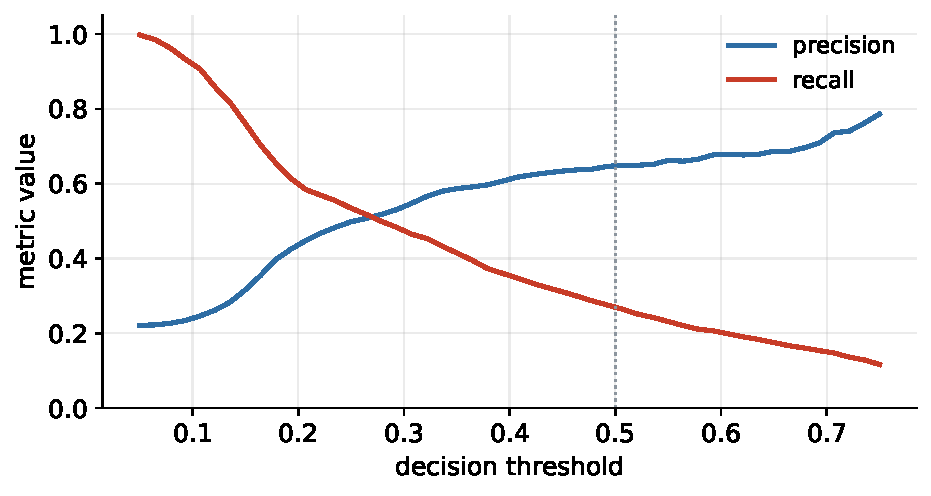
\includegraphics[width=0.62\textwidth]{lecture_2/figures/fig_threshold_tradeoff.pdf}
\caption{Precision and recall as the decision threshold moves.}
\label{fig:threshold}
\end{figure}

Notice the division of labour the pair encodes, because each answers a
different stakeholder. Precision speaks to the \emph{cost of acting}: of
the customers we decline (or route to manual review), how many deserved
it? - the number the customer-experience side and the false-alarm
budget care about. Recall speaks to the \emph{cost of missing}: of the
losses coming toward us, what share did we intercept? - the number the
risk appetite statement cares about. Reporting one without the other is
how models get gamed: a model can reach precision near 100\% by
flagging only its three most obvious defaulters (recall collapses), or
recall of 100\% by flagging everyone (precision collapses to the base
rate). Any single-number summary of the pair, F1 included, has silently
chosen an exchange rate between the two - and F1's choice (equal
weight, harmonic mean, true negatives invisible) corresponds to no
bank's economics. When you must compress, compress with the cost
arithmetic above, where the exchange rate is at least stated in money.

\subsubsection{The bridge to Block 3: from thresholds to ranking}
Every number in this section shares one confession: it depends on the
threshold, and we have just seen the threshold is a business variable,
not a model property. So how do you evaluate the \emph{model itself},
before and apart from any threshold choice? Ask a question no cut-off
can distort: take a random defaulter and a random good customer - how
often does the model assign the defaulter the higher PD? That
probability is threshold-free, insensitive to the base rate, and
measures exactly the quality that made our 80.6\%-accuracy model worth
defending: ranking. It is called AUC, it is the headline metric of PD
model validation, and Block 3 builds it properly from the ROC curve -
where our baseline will post an AUC of 0.731, a number to remember,
because every fancier model in the rest of the course will be asked one
question first: did you beat it?

Which metric for PD, then? Accuracy: no. Precision and recall: honest but
threshold-bound - they judge one cut-off, not the model. What we actually
want, in order: does the model \emph{rank} risk well (ROC/AUC)? are the
probabilities \emph{honest} (calibration)? what does the best threshold
\emph{earn} (expected cost)? All three arrive in Block 3. Until then, one
rule survives every situation: never a single metric, never on training
data.

\subsection{Lab and hand-in}
The lab notebook \texttt{02\_regression\_baselines} walks the block's arc
on the live portfolio: a stratified, seeded split; the linear warm-up with
its residual check; the logistic PD baseline inside a pipeline;
coefficients and odds ratios (with the Block 1 indicator on top); the
accuracy trap on the student's own numbers; confusion matrices at two
thresholds; and an optional sweep of \texttt{C} to watch the leash work.
Exercises add one-hot \texttt{purpose}, a recall-targeted threshold, a
refit without the indicator (watch correlated teammates absorb its role),
and the clean in-pipeline imputation. ``Done'' means being able to defend
the baseline: features used, one number you trust, and why. The project
checkpoint: teams close at Block 3, the data-understanding note is due
before it, and the rubric's ``$\geq 2$ model families, justified'' expects
one of them to be exactly this kind of baseline.

A closing word on what ``one number you trust'' means, because it is the
block's whole argument in miniature. It is not the highest number your
notebook produced; it is a number whose provenance you can narrate under
questioning: computed on held-out data the model never touched, with
every transform fitted inside the pipeline, at a threshold you chose for
a stated reason, read alongside the base rate it must beat, and carried
with its sampling uncertainty rather than its third decimal. A student
who can tell that story about one honest number has understood Block 2;
next week we make the story stronger - cross-validation to steady the
estimate, AUC to free it from the threshold, and one engineered trap to
test whether the discipline holds when the leak is hiding inside a
plausible-looking feature.

% =====================================================================
\section{Block 3 - Trees, ensembles \& honest evaluation}

Block 2 left a challenge on the table: a logistic baseline with test AUC
0.731 on 30{,}000 real clients, and a rule that complexity must earn its keep. Block 3 supplies the
challengers - trees and their ensembles - and, more importantly,
upgrades the judging: cross-validation, ROC/AUC, calibration, and a
threshold with a price tag. It also detonates, deliberately, the leakage
trap armed in Block 1.

The block has a deliberate arc, and it helps to see it whole before
diving in. First come the models that bend: a single decision tree, an
interlude on support vector machines (the third classical route to
nonlinearity), and then the ensembles - random forests and gradient
boosting - that turned trees into the workhorses of tabular machine
learning. Then, precisely because the models get stronger, the judging
must get stronger too: a single train/test split will no longer carry
the weight of the decisions we want to make, so cross-validation,
ranking metrics, calibration and expected cost arrive as a matched set.
And finally, the block's darkest lesson: a model can pass every one of
those upgraded checks and still be worthless, because the checks share
a blind spot called leakage. Keep that arc in mind - each section
exists because the previous one created a need it could not satisfy.

\subsection{Models made of rules: decision trees}
Where logistic regression draws one straight boundary, a decision tree asks
nested yes/no questions: \emph{if utilisation exceeds 0.62, and there is no
checking account, risk is high; otherwise\ldots} Each question splits the
data; each leaf holds a prediction (the leaf's default rate). Two properties
follow immediately. Trees read like a \emph{credit policy}, which is why
business audiences trust them instantly. And because the second question
applies only inside the first question's branch, trees model
\textbf{interactions natively} - Block 2's hand-built product columns,
for free. Geometrically (Figure~\ref{fig:bound3}), logistic regression cuts
the feature space once; a tree tiles it with axis-aligned rectangles.

\begin{figure}[htbp]
\centering
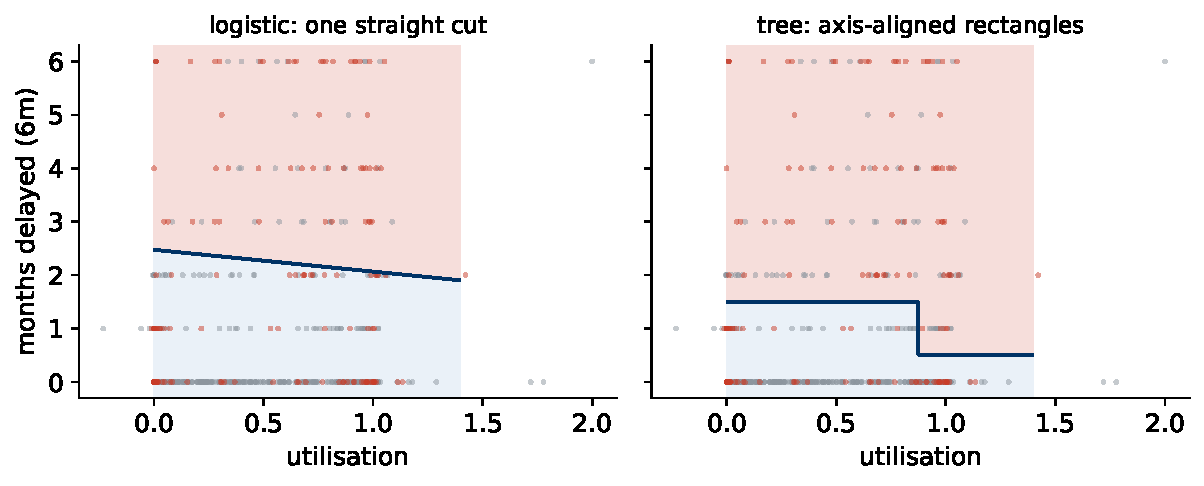
\includegraphics[width=0.78\textwidth]{lecture_3/figures/fig_boundaries.pdf}
\caption{Same two features: one straight cut versus axis-aligned
rectangles.}
\label{fig:bound3}
\end{figure}

\begin{figure}[htbp]
\centering
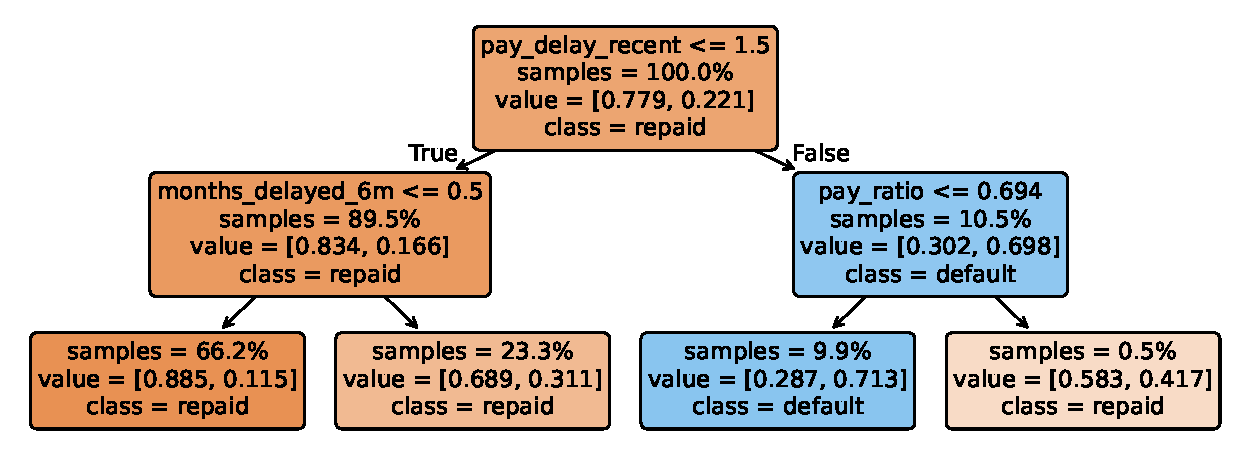
\includegraphics[width=0.9\textwidth]{lecture_3/figures/fig_tree_example.pdf}
\caption{A depth-2 tree fitted to the portfolio. The root split is the
recent repayment status - the tree agrees with the logistic model about
where the signal lives.}
\label{fig:tree3}
\end{figure}

Figure~\ref{fig:tree3} shows a small tree fitted to the portfolio.
Prediction means walking one path from root to leaf, and reading the path
aloud is an explanation for free. Note the root: the tree opens on
\texttt{pay\_delay\_recent} at the two-months-behind cliff - agreeing
with the logistic coefficients that payment history is where the signal
lives. Two very different algorithms, the same verdict. When two model
families that share no assumptions point at the same feature, you have
learned something about the \emph{data}, not just about a model - and
that kind of agreement is worth more than a tenth of a point of AUC.

\subsubsection{Recursive partitioning as greedy optimisation}
It pays to be precise about what the tree-growing algorithm actually
optimises, because the answer explains both its speed and its blind
spots. The object we would \emph{like} to find is the best tree overall:
the partition of the feature space into rectangles that minimises some
loss on the training data, subject to a size limit. That problem is
computationally hopeless - the number of distinct trees explodes
combinatorially with depth and the number of features, and finding the
optimal tree is NP-hard even in stylised versions. So CART and its
descendants settle for a \textbf{greedy} strategy: at every node, choose
the single split that looks best \emph{right now}, commit to it, and
recurse into the children without ever reconsidering. No lookahead, no
backtracking. One pass over features and cut-points per node, and the
whole tree is grown in seconds even on our 21{,}000 training rows.

Greed is a trade, and the price is that the algorithm can miss
structure that only pays off two moves ahead. The classic worked
example is an XOR-style interaction. Imagine two binary flags, $A$ and
$B$, and a toy world where a customer defaults exactly when \emph{one}
of the flags is up but not both. Check the marginals: splitting on $A$
alone gives two children that are each still 50/50 - zero impurity
gain. Splitting on $B$ alone: identical, zero gain. To the greedy
criterion both features look useless, even though together they
determine the outcome \emph{perfectly} - because the value of asking
about $A$ only materialises after you have asked about $B$, and vice
versa. If the tree does split on one of them anyway (a noisy
tie-break, a slight imbalance in the sample), the other feature
becomes perfectly informative inside each branch and the tree finishes
the job; if not, the interaction is simply never found. Pure XOR is
rare in credit data, but softened versions - features that matter
only inside a segment - are everywhere, and greedy growth finds them
only when the path to them happens to open. This is one honest reason
why ensembles of many differently-grown trees, which explore many
different first moves, see things a single greedy tree does not.

\subsubsection{Impurity: Gini, entropy, and a worked split}
Splits are chosen greedily; the criterion that scores them is
\textbf{impurity}. At every node the algorithm tries every feature and
every cut-point and keeps the split that makes the children purest,
measured by Gini impurity $1 - p_0^2 - p_1^2$, where $p_k$ are the
class shares in the node: a pure leaf scores 0, a 50/50 node scores
0.5. A worked example fixes it. A parent node of 1{,}000
customers at 30\% default has Gini $1 - 0.7^2 - 0.3^2 = 0.42$; splitting on
utilisation $> 0.6$ into 600 customers at 10\% (Gini 0.18) and 400 at 60\%
(Gini 0.48) gives weighted impurity $0.6 \times 0.18 + 0.4 \times 0.48 =
0.30$, an improvement of $0.12$. Now score a weaker candidate against
it, because the comparison is the point: splitting the same parent on
age $> 40$ into two children of 500, at 25\% and 35\% default, gives
Ginis $1 - 0.75^2 - 0.25^2 = 0.375$ and $1 - 0.65^2 - 0.35^2 = 0.455$,
weighted impurity $0.5 \times 0.375 + 0.5 \times 0.455 = 0.415$, an
improvement of only $0.005$. The utilisation split separates risk; the
age split shuffles it. The algorithm computes that improvement
for every candidate split, takes the maximum - utilisation wins by a
mile - and growth recurses until a stopping rule intervenes.

Entropy, $-\sum_k p_k \log_2 p_k$, is the same idea with logarithms,
and the two rarely rank splits differently. You can verify that on the
same example: the parent's entropy is
$-(0.3 \log_2 0.3 + 0.7 \log_2 0.7) \approx 0.881$; the utilisation
children score about $0.469$ and $0.971$, weighted $\approx 0.670$,
for a gain of $\approx 0.211$ - the same clear winner, on a different
scale. The deeper reason the rankings agree is that both measures are
concave functions of the class share, both peak at 50/50, both hit
zero at purity, and their curvatures differ only mildly in between; a
split has to be finely balanced on the boundary of two candidates
before the choice of measure flips the decision. In practice you leave
the criterion at its default and spend your attention where it
matters: on the leash.

\subsubsection{Growing, stopping, and the classical leash}
That stopping rule is the tree's leash -
\texttt{max\_depth}, \texttt{min\_samples\_leaf}, pruning - and
Figure~\ref{fig:depth3} shows the familiar U-curve: unleashed, training AUC
approaches 1 while test AUC falls; on this portfolio the optimum sits around
depth 6 - thirty thousand rows feed a deeper tree than four thousand
ever could. The mechanics of memorisation are worth spelling out once:
an unleashed tree keeps splitting until leaves hold a handful of
customers each, and a leaf of three customers ``predicts'' whatever
those three happened to do - noise, dressed as a rule. Depth limits
and minimum leaf sizes prevent the noise-leaves from forming in the
first place.

\begin{figure}[htbp]
\centering
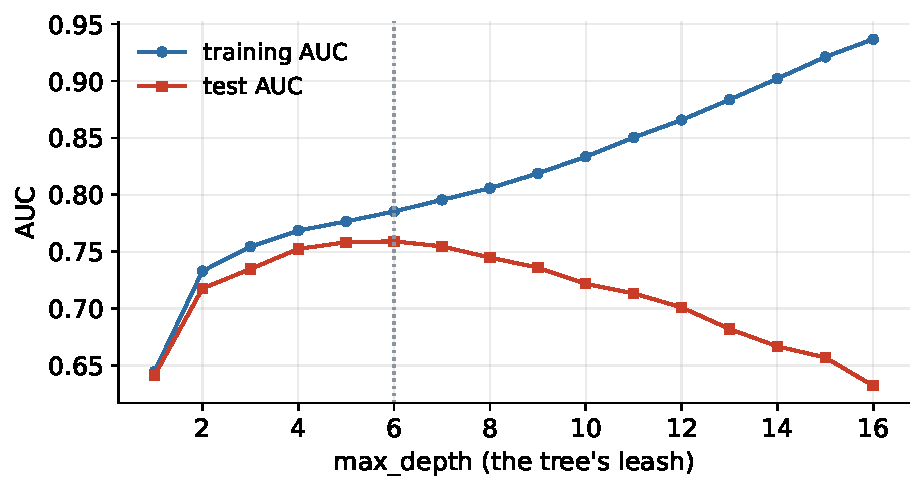
\includegraphics[width=0.6\textwidth]{lecture_3/figures/fig_tree_depth.pdf}
\caption{The U-curve, tree edition: \texttt{max\_depth} is the leash.}
\label{fig:depth3}
\end{figure}

The classical alternative to stopping early is \textbf{cost-complexity
pruning}: grow the tree deliberately too large, then cut it back. The
pruning criterion should look familiar from Block 2 - it is loss plus
leash again: minimise (training error) $+\ \alpha \times$ (number of
leaves), where $\alpha$ prices every leaf the tree wants to keep. At
$\alpha = 0$ the full tree survives; as $\alpha$ grows, subtrees whose
error reduction does not justify their leaf count are collapsed back
into single leaves, and the tree shrinks along a nested sequence of
candidates; $\alpha$ itself is chosen by cross-validation. Pre-stopping
(\texttt{max\_depth}) is cheaper and is what most practitioners tune;
pruning is the more principled classical answer because it lets a
locally-unpromising split survive when its \emph{descendants} earn the
keep - a partial antidote to greed. Either way, the leash logic is
identical to the $\alpha$ of ridge and lasso: a complexity price,
tuned on data the model has not seen.

\subsubsection{Why one tree is not enough}
A single tree has three pathologies worth naming. \emph{High variance}:
nudge the training data and the first split flips, and everything below it
changes - one tree is a nervous model. This instability is structural,
not incidental. The greedy chain means every split is conditioned on
all the splits above it, so a small perturbation at the root -
a few resampled rows moving a cut-point, two nearly-tied candidate
features swapping ranks - does not produce a slightly different tree;
it produces a \emph{different tree}, with different rules, different
leaves, and visibly different predictions for individual customers. If
you bootstrap the training set ten times and grow ten trees, you will
often get ten different root features and ten stories a risk committee
would struggle to reconcile. Hold that thought: an estimator whose
errors swing wildly around the truth is exactly the kind of estimator
that \emph{averaging} can rescue, and that single observation is the
seed of everything in the ensembles section. \emph{Steps, not slopes}:
within a leaf the prediction is constant, so risk that plainly grows with
utilisation becomes a staircase. \emph{Extrapolation, worse edition}:
beyond the training range a tree predicts the edge leaf's value, flat
forever. Regression trees share all of this with a numeric target -
leaves predict means, splits minimise variance - and matter today chiefly
because gradient boosting fits regression trees to errors even for
classification.

What trees \emph{don't} need is almost as instructive. No scaling (splits
compare against cut-points; units are irrelevant); no monotone transforms
(the log-income lens changes nothing - splits are order-based); no
one-hot gymnastics for ordinal codes (a tree can cut an ordered code
anywhere, and the dummy trap is a linear-model disease). Missing values:
plain sklearn trees still require imputation, but
\texttt{HistGradientBoosting} handles NaN natively, learning which side a
missing value should travel - Block 1's structural NaN can stay a NaN.
Less preprocessing does not mean less thinking: the time-travel test and
the missingness taxonomy apply in full. The invariance to monotone
transforms deserves one more sentence, because it is a genuinely deep
property: a split at income $> 50{,}000$ and a split at
$\log(\text{income}) > \log(50{,}000)$ partition the customers
identically, so the entire tree - structure, predictions,
everything - is unchanged by any order-preserving relabelling of a
feature. All the anguish Block 2 spent on skew, outliers and feature
scaling simply does not arise; what remains, undiminished, is the
anguish about \emph{which features are legitimate}.

\subsection{Interlude: support vector machines}
Before the ensembles, a brief visit to the third classical route to
nonlinearity - and a beautiful piece of geometry. Among all lines that
separate two classes, the \textbf{support vector machine} picks the one
with the widest margin:
\[
  \min_{w, b}\; \tfrac{1}{2}\lVert w \rVert^2
  \quad \text{s.t.} \quad y_i (w \cdot x_i + b) \geq 1 ,
\]
whose margin width is $2 / \lVert w \rVert$; the soft-margin version adds
$C \sum_i \xi_i$ to tolerate violations, with $C$ as the leash. The
striking property (Figure~\ref{fig:svmmargin}): the boundary is held up
only by the \emph{support vectors}, the circled border cases - every
other customer could vanish without moving the line. A wide street is
built-in caution about new customers near the boundary.

\begin{figure}[htbp]
\centering
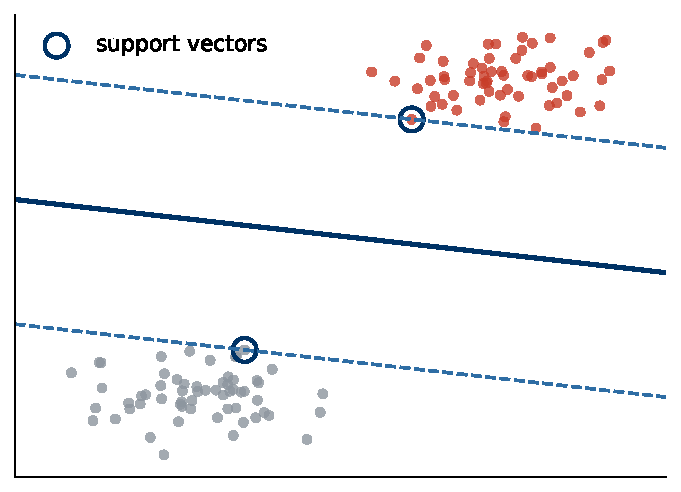
\includegraphics[width=0.44\textwidth]{lecture_3/figures/fig_svm_margin.pdf}
\caption{Maximum margin: the boundary rests on the support vectors alone.}
\label{fig:svmmargin}
\end{figure}

\subsubsection{The margin is a leash}
Look again at the objective and you will recognise an old friend
wearing a new costume. Minimising $\lVert w \rVert^2$ is exactly the
ridge penalty from Block 2; the SVM has merely moved the data-fitting
part into the constraints. A small $\lVert w \rVert$ means the decision
function changes slowly across the feature space - a flat, cautious
function - and, since the margin width is $2/\lVert w \rVert$, a small
norm \emph{is} a wide margin. Margin maximisation is regularisation,
stated geometrically. This is why the soft-margin trade-off behaves
exactly like every leash in this course: large $C$ punishes margin
violations harshly, the street narrows to accommodate every borderline
training customer, and the model memorises; small $C$ keeps the street
wide, tolerates some misclassified training points, and generalises.
The statistical-learning-theory result that made SVMs famous says the
same thing formally: generalisation bounds for large-margin classifiers
depend on the margin achieved, not on the dimension of the space - a
license to work in absurdly high-dimensional feature spaces, which the
next idea promptly exploits.

\subsubsection{The kernel trick and its economics}
Nonlinearity arrives via the \textbf{kernel trick}: map points into a
higher-dimensional space where a line suffices, computed implicitly
through a kernel $K(x, x') = \varphi(x) \cdot \varphi(x')$ without ever
building $\varphi$. The economics of that sentence deserve unpacking,
because they are the whole trick. Suppose you wanted the degree-2
polynomial expansion of $p = 100$ features explicitly: all squares and
pairwise products, roughly $p(p+3)/2 \approx 5{,}150$ columns; at
degree 5 the count runs into the tens of millions, and the RBF
kernel's implicit feature space is infinite-dimensional - you could
not build it if you wanted to. Yet the kernel evaluates the dot
product \emph{in} that space with a formula that touches only the
original $p$ coordinates: for RBF, one squared distance and one
exponential. Because the SVM's optimisation and its final decision
function can both be written entirely in terms of dot products between
data points, replacing every dot product with $K$ trains a linear
model in the giant space at the price of the small one. The trick's
economics cut both ways, though: the cost now scales with the
\emph{number of rows} rather than the number of features - the
kernel matrix is $n \times n$ - which is precisely the $n^2$ wall
the method hits on large datasets. The workhorse RBF kernel,
$K(x, x') = \exp(-\gamma \lVert x - x' \rVert^2)$, encodes similarity
decaying with distance - and $\gamma$ is one more leash: large
$\gamma$ makes similarity hyper-local (every training point its own
island, memorisation), small $\gamma$ blurs everyone together (back
towards a linear model).
Figure~\ref{fig:svmkernel} shows the effect on the course's crescents:
the linear kernel is still a line; the RBF machine bends.

\begin{figure}[htbp]
\centering
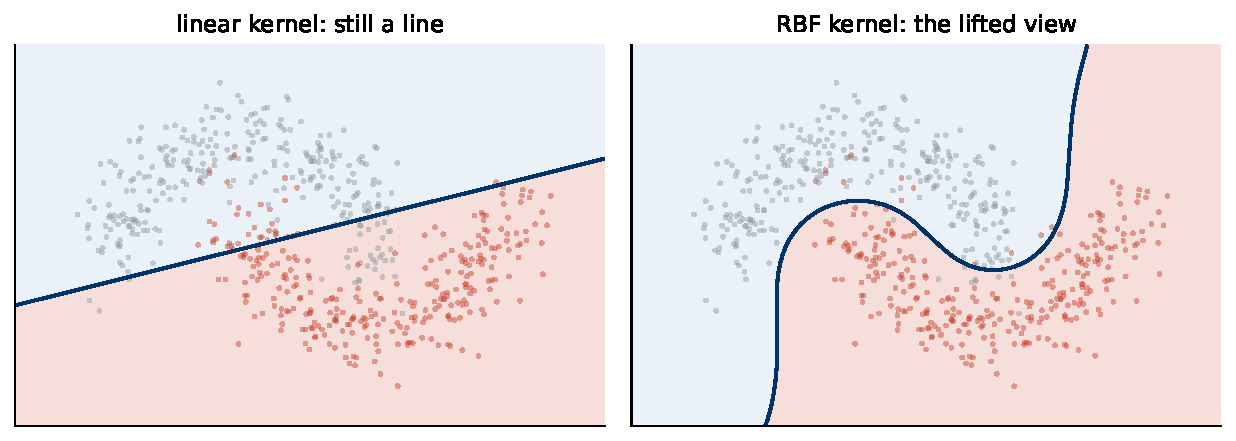
\includegraphics[width=0.76\textwidth]{lecture_3/figures/fig_svm_kernel.pdf}
\caption{The kernel trick on the crescents: linear versus RBF.}
\label{fig:svmkernel}
\end{figure}

\subsubsection{Hinge versus logistic loss}
In loss-function terms the SVM minimises the \emph{hinge loss}
$\max(0,\, 1 - y f(x))$, which is zero once a point is right \emph{with
margin} - against Block 2's logistic loss, which never fully forgives
(Figure~\ref{fig:losses3}); both are convex stand-ins for the 0/1 loss we
actually care about, and the whole model is once again loss plus leash,
minimised. The difference in forgiveness has consequences. Because the
hinge is exactly zero for confidently-correct points, they drop out of
the optimisation entirely - that is \emph{why} only the support
vectors hold up the boundary, restated in loss language. The logistic
loss, by contrast, keeps a small gradient alive for every customer, no
matter how safely classified; every point pulls on the coefficients a
little, forever. One practical corollary matters for credit: the
logistic loss's gentle slope is what makes its outputs interpretable
as probabilities, while the hinge's hard zero produces a margin score
with no probability semantics at all - the geometric elegance costs
you the PD.

\begin{figure}[htbp]
\centering
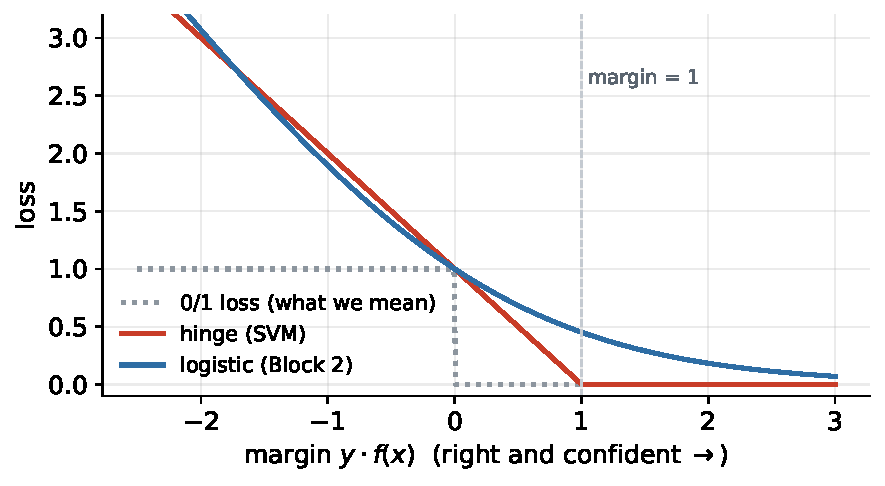
\includegraphics[width=0.56\textwidth]{lecture_3/figures/fig_losses.pdf}
\caption{Three losses against the margin $y f(x)$: 0/1, hinge, logistic.}
\label{fig:losses3}
\end{figure}

In practice: scale first (distances again); no native probabilities
(calibrate before pricing - the SVM outputs margins, not PDs); and
training scales poorly past $\sim 10^5$ rows, one reason GBDT took the
tabular crown SVMs wore in the 2000s. On our PD task - trained on a
6{,}000-row subsample precisely because of that $n^2$ cost - the RBF SVM
scores test AUC 0.715, behind even the logistic baseline: kernels buy
bend, but not as cheaply as trees buy the delay cliff. The fuller
verdict on why SVMs faded on tabular data lists four counts: the
$n^2$ cost; no native probabilities; no native handling of missing
values or categoricals, both endemic in business data; and two
sensitive leashes ($C$, $\gamma$) that must be grid-searched where
GBDT's defaults already land close. But note what \emph{survived} the
fashion cycle, because it is most of the intellectual content: margins
as a lens for understanding generalisation (the standard explanation
for why boosting resists overfitting is a margin argument), kernels as
the general recipe for making linear methods nonlinear (kernel ridge,
kernel PCA, Gaussian processes), and the discipline of writing every
model as loss plus leash. Methods fade; ideas migrate.

\subsection{Ensembles: manufacturing disagreement}
One tree is nervous; a crowd of \emph{differently-wrong} trees is calm.
Averaging many over-flexible models cancels part of their individual
errors: variance drops, bias stays. The catch is that trees grown on the
same data make the same mistakes - averaging clones buys nothing - so
ensembling is really the art of manufacturing \emph{disagreement} between
good models and averaging it away. Two recipes dominate: give each tree
different \emph{data} (bagging), or give each tree a different
\emph{job} (boosting). Everything in this section is one of those two
moves, plus engineering.

\subsubsection{Bagging: the bootstrap variance-reduction argument}
\textbf{Bagging} gives each tree different data: bootstrap-sample $n$ rows
with replacement (each tree sees $\sim$63\% of unique rows), grow deep,
average the probabilities. The 63\% is not folklore: the chance one
particular row escapes all $n$ draws is $(1 - 1/n)^n \to e^{-1}
\approx 0.368$, so about 63.2\% of distinct rows make it into each
bootstrap sample and about 37\% sit out. Each tree's unseen $\sim$37\%
(the \emph{out-of-bag} rows) supplies validation-like feedback without a
split: score every row using only the trees that did \emph{not} train
on it, and you get an honest generalisation estimate as a by-product
of training - free validation, no held-out data spent.

Why does averaging help, and by how much? The statistics of averages
tell the whole story, and it is worth telling in words. Average $B$
estimators that each have the same error variance. If their errors
were \emph{independent}, the variance of the average would shrink like
$1/B$ - the classic ``average of noisy measurements'' effect, and
with hundreds of trees the nervousness would essentially vanish. But
bootstrap trees are not independent: they are grown on overlapping
samples of the same portfolio, so their errors are \emph{correlated},
and the variance of the average splits into two parts - a part
proportional to the between-tree correlation, which averaging cannot
touch, and a part that decays like $1/B$, which averaging kills. Add
trees and the second term dies; what remains is a variance
\emph{floor} set entirely by how correlated the trees are. Read that
formula-in-words twice, because it is the design brief for the random
forest: once you have enough trees, the only remaining lever is
\emph{decorrelation}. Averaging more clones buys nothing; making the
crowd disagree buys everything.

\subsubsection{Random forests: the feature lottery}
A \textbf{random forest} adds a feature lottery: at every node only a
random subset of features (\texttt{max\_features}) may compete. Without
it, one dominant feature opens every bootstrap tree identically and the
trees stay correlated; the lottery forces variety, decorrelates the crowd,
and makes the averaging work. On our portfolio the dominant feature is
obvious - the repayment-status cliff - and without the lottery
nearly every bootstrap tree would open on it, agree about the top of
the tree, and disagree only in the noisy lower branches: exactly the
high-correlation regime where averaging stalls at its floor. Forcing
some root splits to choose among other features (utilisation, limits,
history) produces trees that carve the space along genuinely different
first cuts, and their pooled vote is calmer than any of them. The
standard default, \texttt{max\_features} $\approx \sqrt{p}$, is a
sensible compromise: aggressive enough to decorrelate, gentle enough
that most nodes still see \emph{some} strong candidate. Note the
paradox worth savouring: the lottery makes every \emph{individual}
tree worse - it is sometimes forbidden from using the best feature -
and the \emph{ensemble} better. Deliberately handicapping the members
to improve the committee is the deepest idea in this section.

As Figure~\ref{fig:ntrees3} shows, test AUC
climbs and then plateaus in the number of trees - more trees never
overfit, they only cost compute, so \texttt{n\_estimators} is not really a
tuning knob; the tree-level leashes are. The plateau is the variance
floor made visible: by a few hundred trees the $1/B$ term is gone and
the correlation term is all that is left. This is also why the forest
is famously hard to ruin - its members are deep, low-bias trees, its
averaging handles their variance, and the only real leashes
(\texttt{min\_samples\_leaf}, \texttt{max\_features}) have forgiving
defaults.

\begin{figure}[htbp]
\centering
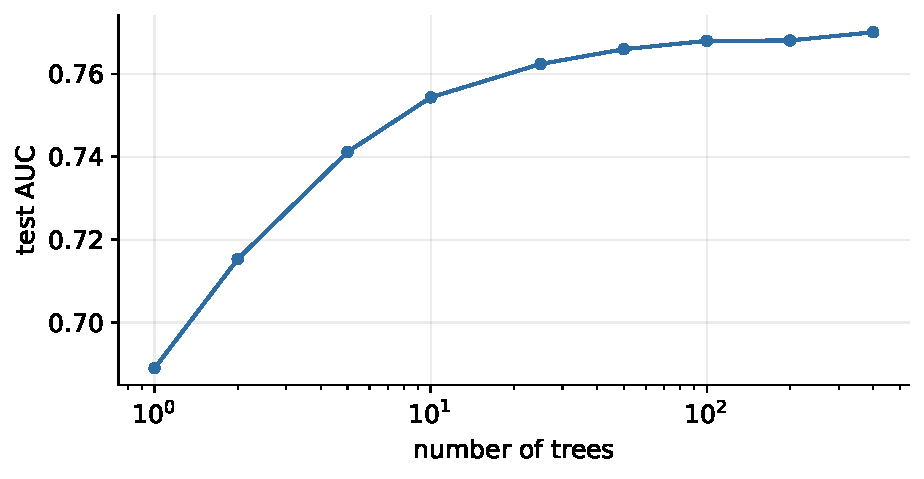
\includegraphics[width=0.58\textwidth]{lecture_3/figures/fig_rf_ntrees.pdf}
\caption{Random forest: more trees plateau, never overfit.}
\label{fig:ntrees3}
\end{figure}

\subsubsection{Boosting: stagewise additive modelling}
\textbf{Boosting} gives each tree a different job: build sequentially, each
new (small, shallow) regression tree fitting the \emph{gradient} of the
loss - the errors of the ensemble so far - with predictions
accumulating as $F_m = F_{m-1} + \eta\,\text{tree}_m$ under a learning
rate $\eta$. The scheme has a classical name, \emph{stagewise additive
modelling}: the final model is a sum of many small terms, fitted one
at a time, each term frozen the moment it is added. No term is ever
revisited - like the greedy tree, boosting commits and moves on - and
the model's capacity grows term by term, which is exactly why the
number of rounds is part of the leash.

One honest paragraph on why it is called \emph{gradient} boosting,
because the name is precise, not decorative. Think of the model's
predictions on the training set as the unknowns - one number per
customer - and the training loss as a function of those numbers.
Gradient descent would improve the loss by nudging each prediction
against its gradient: for log-loss, the gradient for one customer is
(predicted probability minus actual outcome), i.e.\ the residual. But
we cannot ship a lookup table of per-customer nudges - we need the
update to be a \emph{function} that generalises to new customers. So
each round fits a small regression tree to the residuals: the tree is
the best function-shaped approximation of the gradient step that the
tree family can express, and adding $\eta$ times that tree to the
ensemble is one step of gradient descent \emph{in the space of
functions}. Rounds are iterations; the learning rate is the step size;
early stopping is the convergence criterion. This is also why the
regression trees of the tree section matter even for classification -
residuals are numeric, whatever the target was.

Two design choices follow from the mechanics. \emph{Shallow trees}: a
tree of depth $d$ can express interactions of order at most $d$, so
capping depth at 2--4 makes each round a humble, low-order correction
and lets the \emph{sum} build complexity gradually; a deep tree per
round would take huge, overfitting-prone steps. \emph{The learning
rate versus rounds trade-off}: shrinking $\eta$ makes each step
smaller, so more rounds are needed to reach the same training fit -
but the slow path is smoother and reliably generalises better, which
is why the classic recipe is a small learning rate, many rounds, and
early stopping on a validation slice to say when to get off. Where
bagging attacks variance, boosting attacks bias, and can
therefore overfit; its leash (learning rate $\times$ rounds, tree size,
early stopping) matters more. The industrial implementations - XGBoost,
LightGBM, CatBoost - are refinements of exactly this idea:
histogram-binned split search for speed, built-in regularisation
terms, native missing-value and categorical handling, but the same
stagewise gradient skeleton underneath.

\subsubsection{Random forest or gradient boosting?}
Practical guidance, since you will face the choice in the project and
beyond. The forest is the robust first ensemble: parallel, nearly
tuning-free, hard to ruin, and a strong benchmark within minutes - if
your carefully tuned GBDT cannot beat a default forest, your tuning is
not working. GBDT is the usual state of the art on tabular data, but
it earns that title only with its leash held properly: early stopping
on a validation slice, a modest learning rate, shallow trees - it is
easy to ruin, and half its bad reputation in careless hands is
self-inflicted overfitting. The forest's deep trees attack variance by
averaging; boosting's shallow trees attack bias by accumulating - so
the forest is the safer default when data is small or noisy, and
boosting pulls ahead when there is enough signal and enough rows to
support its appetite. On our portfolio the two finish in a statistical
dead heat (0.774 versus 0.773 on the test set), which is itself a
lesson: the gap between well-run ensembles is usually smaller than the
gap between either and a model run carelessly.

\begin{practice}
Leashes are sized to the data. On this 21{,}000-row training set,
sklearn's default GBDT already scores 0.774 - the defaults are tuned for
data of roughly this size. The same defaults on Block 1's 2{,}800-row
synthetic world scored 0.651 against 0.714 tuned: small data needs short
leashes. Check in both directions; never assume.
\end{practice}

\begin{figure}[htbp]
\centering
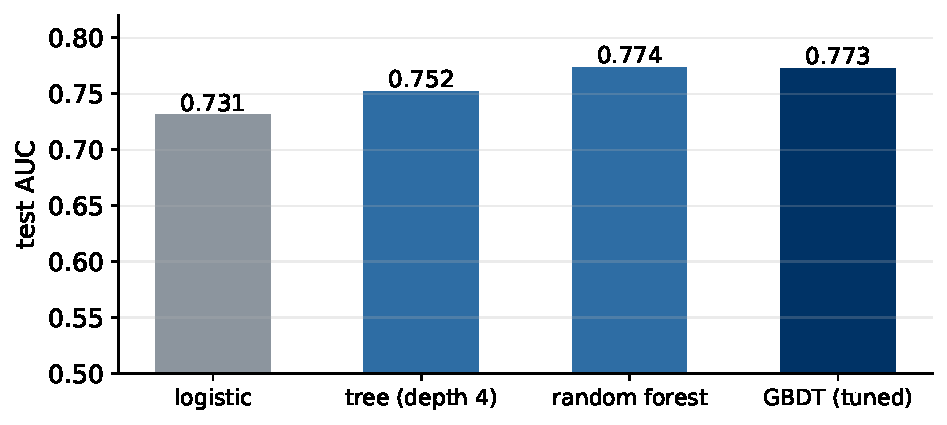
\includegraphics[width=0.62\textwidth]{lecture_3/figures/fig_model_comparison.pdf}
\caption{The tournament on held-out data: every rung of the ladder pays.}
\label{fig:tournament3}
\end{figure}

The tournament (Figure~\ref{fig:tournament3}) delivers the block's
headline: every rung of the ladder pays. Logistic 0.731, a single
depth-4 tree 0.752, random forest 0.774, tuned GBDT 0.773 - about four
AUC points from baseline to ensemble, on real behavioural data full of
exactly what linear models must be hand-fed: the repayment-status cliff
(one missed month is news, the second is a siren), saturating
utilisation, delay-by-limit interactions. The contrast with Block 1's
synthetic world - additive in log-odds by construction, where the
baseline held and complexity politely declined - is the meta-lesson in
stereo: which family wins is an empirical question, decided per dataset,
against a baseline, on honest numbers, never by fashion. On tuning: start from defaults and move one leash at a
time; random search beats grid search at equal budget; tune on
cross-validation and confirm on test; and stop early - feature work
usually pays more than the fourth hour of tuning.

\subsection{Evaluation you can trust}
The tournament just ranked four models on one held-out test set, and
the honest question is: how much should you trust that ranking? To
answer it you need to know what a single split actually measures.

\subsubsection{What one split estimates - and its variance}
When you compute test AUC on one train/test split, you are estimating
a population quantity - roughly, ``how well would this model rank
future customers drawn from the same portfolio?'' - using one finite
sample of test rows and one particular assignment of rows to sides.
Both choices inject randomness. A different lottery of rows into the
test set would contain different hard cases and different flukes, and
the number would move; a different training draw would fit a slightly
different model, and the number would move again. The single split's
score is therefore a draw from a distribution - a random variable
pretending to be a number - and its spread shrinks with the test
set's size. Our test set of 9{,}000 customers keeps the noise modest,
but differences of a few tenths of a point of AUC can still be
sampling luck rather than model quality, and most real projects have
far fewer rows to spend. Two conclusions follow. First, never let a
single-split difference smaller than the noise decide anything.
Second, to \emph{see} the noise, you need more than one number - you
need a distribution of scores. That is what cross-validation
manufactures.

\subsubsection{$k$-fold cross-validation, slowly}
What cross-validation \emph{is} deserves a slower paragraph than it
usually gets, because it is the single most-used evaluation device in
applied machine learning. The problem it solves: any single test split is
one draw from the space of possible splits, so the score it produces is a
random variable pretending to be a number - and differences of a point of
AUC between models can be pure sampling luck. The device: split the
\emph{training} data into $k$ equal folds (five or ten in practice);
train on $k-1$ of them and score the held-out fold; rotate until every
fold has served as the judge exactly once. Three properties make this
efficient and honest at the same time. Every row is scored by a model
that never saw it, so no score is contaminated by memorisation. Every row
is used for training in $k-1$ of the rounds, so no data is wasted - the
crucial advantage over carving out a single fixed validation set. And the
output is $k$ scores rather than one, i.e.\ a mean \emph{and a spread},
which is what turns model comparison from impression into measurement.
The price is $k$ model fits, and a subtlety worth knowing: the $k$ scores
are not independent (their training sets overlap heavily), so the naive
standard error is optimistic - treat the spread as a readable yardstick,
not a formal confidence interval. Variants tune the trade-offs:
stratified $k$-fold preserves class rates per fold (our default);
repeated CV re-runs the whole procedure with new shuffles when a decision
is close; leave-one-out is the $k = n$ extreme (nearly unbiased,
expensive, high-variance); and nested CV wraps one CV for hyperparameter
tuning inside another for evaluation, the belt-and-braces protocol when
the same data must both choose and judge a model.
Figure~\ref{fig:cv3} shows ours: logistic $0.745 \pm 0.010$, tree
$0.766 \pm 0.008$, forest $0.783 \pm 0.007$ - at 21{,}000 training rows
the spreads are tight, and the tree-versus-logistic gap clears its spread
several times over. The ladder's wins are certified, not lucky; a model
``winning'' by less than the spread has not won anything yet.

\begin{figure}[htbp]
\centering
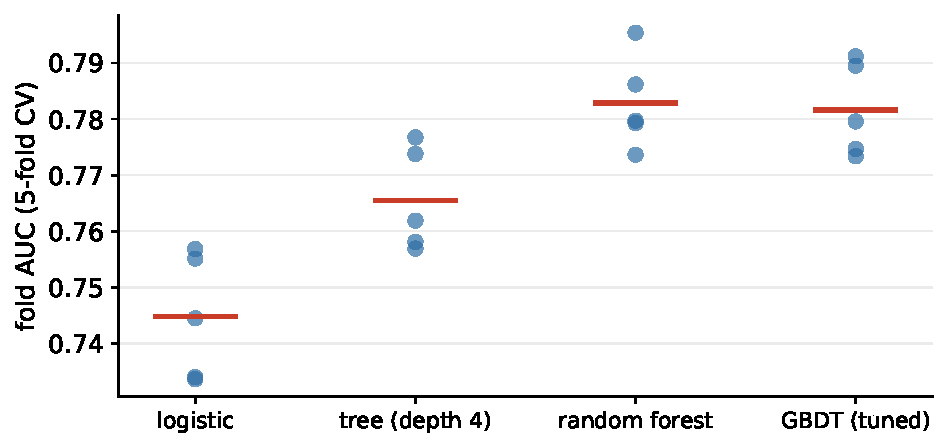
\includegraphics[width=0.6\textwidth]{lecture_3/figures/fig_cv_spread.pdf}
\caption{Five-fold CV: means and spreads - the ladder's gaps clear the
noise.}
\label{fig:cv3}
\end{figure}

\subsubsection{The pipeline goes inside: CV hygiene}
Four rules of CV hygiene. Stratify the folds. Put the \emph{pipeline}
inside the CV so scalers, imputers and encoders are refit per fold -
fitting transforms once on all data leaks across every fold boundary,
which is the real reason pipelines exist. Let CV choose (hyperparameters,
model family) and the untouched test set confirm. And never cross-validate
on data that includes the test set.

The pipeline rule earns a worked example, because the mistake is the
single most common leak in student projects and it looks completely
innocent. Innocent version first: z-score all 21{,}000 training rows
once, \emph{then} run five-fold CV on the scaled matrix. Each fold's
``unseen'' rows have already contributed to the mean and standard
deviation the model trains under - a whisper of the held-out data
inside every fit. For plain scaling the optimism is usually small.
Now the dangerous version: \emph{target mean encoding}, where a
categorical column is replaced by the average default rate of its
category. Fit that encoder once on all rows and every customer's own
outcome flows into their own feature. Take the extreme case to see
it starkly: a category containing a single customer who defaulted
gets the encoded value 1.0 - the label, photocopied into a feature
column - and CV will duly report a spectacular score for a model that
has learned to read its own answer sheet. Fit the encoder inside each
fold, on that fold's training part only, and the fold's held-out rows
are encoded with averages computed \emph{without} them - honest
again. The mechanical rule that prevents the whole class of errors:
anything with a \texttt{fit} method belongs inside the pipeline, and
the pipeline belongs inside the CV loop.

One more split subtlety is
credit-specific: portfolios \emph{drift} (products, policies - Block 1's
selection bias - and the economy), so random CV, which lets the model
``see the future'', scores optimistically. The industry standard is
\textbf{out-of-time validation}: train on the past, test on a later window,
with CV inside the training period for tuning. Our synthetic portfolio has
no dates; your project data or your first job will. Ask ``does time
matter here?'' before every split - for credit the answer is
essentially always yes.

\subsubsection{The ROC curve, built by hand}
Precision and recall judged the model at one threshold. The threshold
belongs to the business and may move, so judge the \emph{ranking} first:
sweep the threshold and trace true-positive rate against false-positive
rate - the \textbf{ROC curve} (Figure~\ref{fig:roc3}), on which choosing
an operating point \emph{is} choosing a threshold.

To demystify the curve completely, build one by hand. Five customers:
three eventual defaulters scored $\{0.9, 0.6, 0.4\}$, two good clients
scored $\{0.5, 0.2\}$. Sort by score, descending:
$0.9\,(\text{bad})$, $0.6\,(\text{bad})$, $0.5\,(\text{good})$,
$0.4\,(\text{bad})$, $0.2\,(\text{good})$. Start with the threshold
above every score: nothing is flagged, so TPR $= 0$, FPR $= 0$ -
the curve's bottom-left corner. Now lower the threshold one score at
a time. Past 0.9: one of three defaulters caught, no false alarms -
$(\text{FPR}, \text{TPR}) = (0, 1/3)$. Past 0.6: $(0, 2/3)$. Past
0.5: the first good client is flagged - $(1/2, 2/3)$; the curve
steps right. Past 0.4: $(1/2, 1)$. Past 0.2: $(1, 1)$, the top-right
corner. Every defaulter passed moves the curve \emph{up}; every good
client passed moves it \emph{right}; a perfect ranking climbs the left
wall before stepping right at all, and a random one staggers up the
diagonal. The area under this little staircase is
$\tfrac{1}{2} \times \tfrac{2}{3} + \tfrac{1}{2} \times 1 = 5/6$ -
hold that number for a moment.

\begin{figure}[htbp]
\centering
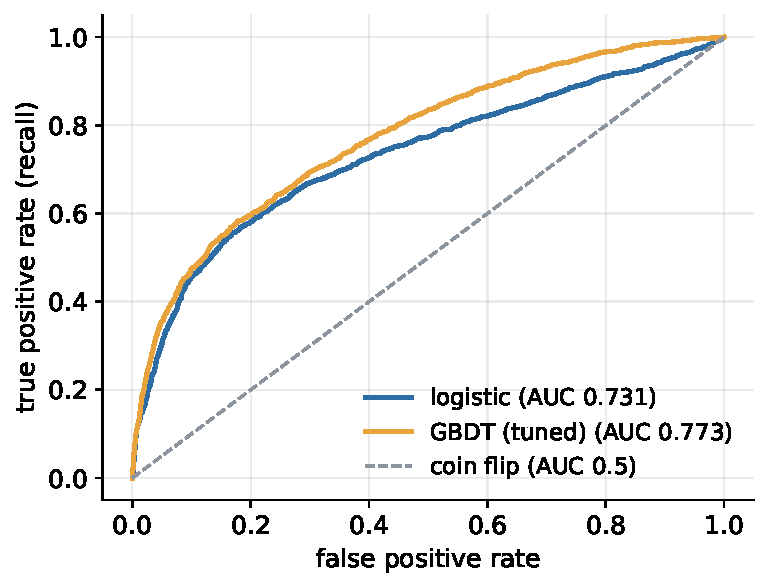
\includegraphics[width=0.5\textwidth]{lecture_3/figures/fig_roc.pdf}
\caption{ROC curves for the baseline and the tuned GBDT.}
\label{fig:roc3}
\end{figure}

The area under the ROC curve has a
meaning worth memorising: \emph{AUC is the probability that a randomly
chosen defaulter is scored riskier than a randomly chosen good customer} -
0.5 is dice, 1.0 a crystal ball, and it is threshold-free and
imbalance-insensitive. What it cannot tell you: whether the probabilities
are honest, or what a decision costs.

\begin{practice}
Credit scoring speaks its own dialect: \textbf{Gini} $= 2\cdot\text{AUC}
- 1$ (logistic 0.46, GBDT $\approx$ 0.55; retail PD models normally live
at 0.4-0.6), and
\textbf{KS}, the maximum gap between the score distributions of goods and
bads. When a risk manager says Gini they mean this - not the Gini
impurity of the tree section. Same Corrado Gini, different formula; knowing
the difference is an interview survival skill.
\end{practice}

\subsubsection{Interpreting AUC and Gini like a practitioner}
Because AUC and Gini decide model approvals, promotions and vendor
contracts, they deserve more than a definition. Start with the
probabilistic reading, because everything else follows from it: AUC is
the probability that a randomly drawn defaulter is scored riskier than a
randomly drawn good client. Our GBDT's 0.773 therefore says: draw one
future defaulter and one future good client at random, and 77 times in
100 the model orders them correctly - 23 times in 100 it has them
backwards. A tiny worked example makes the mechanics concrete: score
three defaulters at $\{0.9, 0.6, 0.4\}$ and two good clients at
$\{0.5, 0.2\}$; of the $3 \times 2 = 6$ defaulter-good pairs, five are
ordered correctly (0.9 and 0.6 beat both good scores, 0.4 beats only
0.2) and none are tied, so AUC $= 5/6 \approx 0.83$ and Gini
$= 2 \cdot 5/6 - 1 = 2/3$. Counting concordant pairs \emph{is} the
metric; the ROC integral is the same count drawn as an area - and
indeed $5/6$ is exactly the staircase area computed by hand above.
Same customers, two routes, one number: that agreement is the proof
that the geometric and probabilistic definitions coincide.

Interpretation then needs anchors, because ``is 0.77 good?'' has no
universal answer - discrimination is a property of the data as much as
of the model. Rules of thumb from retail credit: application scorecards
on bureau-thin data live around Gini 0.3-0.45; mature application
models with bureau data 0.45-0.6; behavioural models - which watch the
customer's own account, like ours - commonly 0.5-0.7 (our 0.55 sits
comfortably here); collections and fraud models can run higher still.
Reading the number against the wrong benchmark produces both false
alarm and false comfort: a Gini of 0.45 is respectable for a thin-file
application model and alarming for a behavioural one, and anything
approaching 0.9 on any credit portfolio is Block 3's leakage smell, not
a triumph. Three more habits keep the metric honest. Quote the
uncertainty (CV spread or a bootstrap interval) - a Gini reported to
three decimals without one is numerology. Compare only within the same
population and time window - AUC shifts when the mix of applicants
shifts, without the model changing at all. And remember what the number
refuses to say: nothing about calibration (Block 3's reliability
diagrams), nothing about the chosen threshold's costs, nothing about
fairness across groups (Block 6). AUC answers exactly one question -
does the model order risk well? - and the practitioner's skill is
refusing to let it answer any other.

\subsubsection{Precision--recall and the tyranny of the base rate}
Two companions complete the ranking view. The \textbf{precision--recall
curve} (Figure~\ref{fig:pr3}) floors at the base rate (22\% here) and
punishes false alarms among rare positives; at real default rates of
1--5\% - or fraud's 0.1\% - ROC can flatter while precision is dismal,
so check both.

Work the base-rate effect in numbers, because nothing else makes it
stick. Take a model operating at a fixed, respectable ROC point: it
catches 80\% of bad customers (TPR $= 0.8$) while flagging 10\% of
good ones (FPR $= 0.1$). At our portfolio's 22\% base rate, among
10{,}000 customers there are 2{,}200 bad and 7{,}800 good; the model
flags $0.8 \times 2{,}200 = 1{,}760$ true positives and
$0.1 \times 7{,}800 = 780$ false alarms, so precision is
$1{,}760 / (1{,}760 + 780) \approx 0.69$ - seven flags in ten are
right, a workable alert queue. Now move the \emph{same model} - same
ROC point, same AUC - to a thin-risk book with a 2\% base rate:
200 bad, 9{,}800 good; it flags $0.8 \times 200 = 160$ true positives
and $0.1 \times 9{,}800 = 980$ false alarms, and precision collapses
to $160 / 1{,}140 \approx 0.14$ - six flags in seven are wrong. The
ROC curve did not move a pixel; the PR curve fell off a cliff. That is
the whole argument for checking both: ROC judges the ranking in a way
that ignores the class mix, which is a feature when you compare models
and a bug when you plan an operation whose workload is made of
\emph{flags}, not of rates.

\begin{figure}[htbp]
\centering
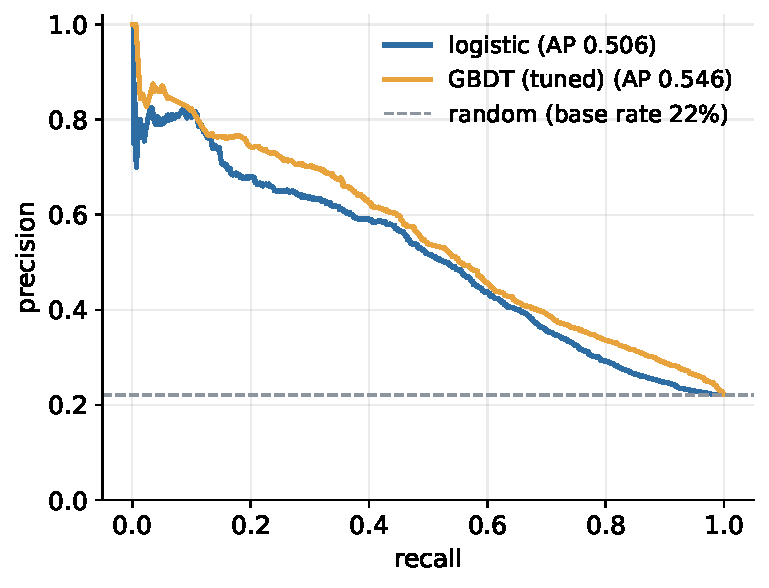
\includegraphics[width=0.5\textwidth]{lecture_3/figures/fig_pr.pdf}
\caption{Precision--recall: random guessing floors at the base rate.}
\label{fig:pr3}
\end{figure}

\subsubsection{Calibration: are the probabilities honest?}
And the \textbf{calibration curve}
(Figure~\ref{fig:cal3}) asks whether a predicted 0.3 defaults 30\% of the
time: ranking pays for approval order, calibration pays for pricing and
provisioning, where the probability itself sets the interest rate. The
diagnostic is the \emph{reliability diagram}: bin customers by
predicted PD (say, deciles), plot each bin's average prediction
against its \emph{observed} default rate, and read the deviations from
the diagonal - points below it mean the model over-states risk in
that range, points above it mean under-statement. Note that
calibration and ranking are genuinely independent virtues: divide
every predicted PD by ten and the ranking (hence AUC) is untouched
while every price computed from the scores becomes nonsense - which
is exactly why the evaluation stack asks the two questions separately.

Repairs
exist (Platt scaling, isotonic regression,
\texttt{CalibratedClassifierCV}) - and they differ in a way worth
knowing. \emph{Platt scaling} fits a small logistic regression mapping
the raw score to a probability: two parameters, hard to overfit, works
on modest data, but it assumes the distortion is sigmoid-shaped.
\emph{Isotonic regression} fits the best monotone step function from
scores to observed rates: assumption-free beyond monotonicity, able to
fix any consistent distortion, but data-hungry - on small samples its
steps chase noise. The practical rule: Platt when calibration data is
scarce, isotonic when it is plentiful; and in both cases fit the
calibrator on data the model was not trained on (the CV-wrapped
estimator does this for you), or the repair inherits the optimism it
was meant to remove. And recall from Block 2 that
\texttt{class\_weight} breaks calibration by design - if you
reweighted classes to help the ranking, recalibrate before anyone
prices with the output.

\begin{figure}[htbp]
\centering
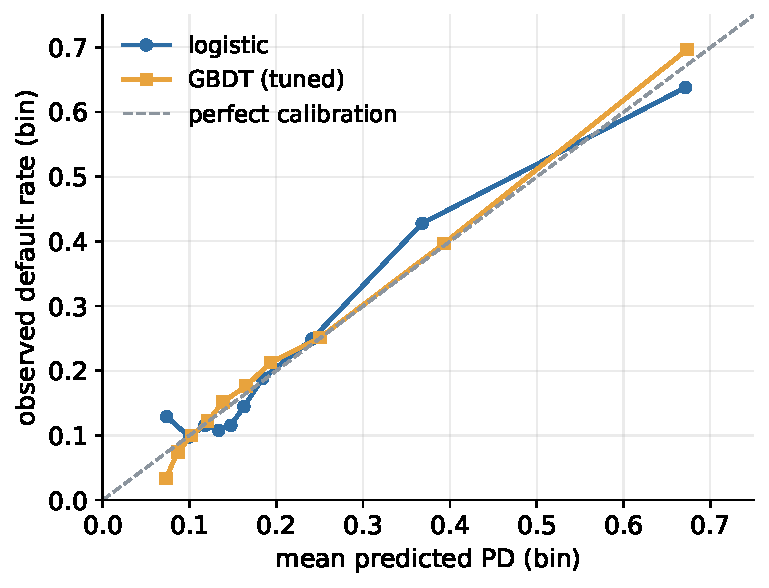
\includegraphics[width=0.5\textwidth]{lecture_3/figures/fig_calibration.pdf}
\caption{Reliability diagram: predicted versus observed default rates.}
\label{fig:cal3}
\end{figure}

\subsubsection{Expected cost: metrics meet money}
Finally, metrics meet money. Price the confusion-matrix cells - here a
missed defaulter at $3\times$ a falsely declined client, deliberately
conservative for our 22\% default rate (real low-default books push
10-50$\times$) - sweep the threshold $t$, and minimise the expected
cost per client,
\[
  \mathrm{E}[\text{cost}](t) =
  \frac{C_{FN}\, FN(t) + C_{FP}\, FP(t)}{n},
  \qquad t^{*} = \arg\min_t \mathrm{E}[\text{cost}](t)
\]
(Figure~\ref{fig:cost3}). The optimum lands near 0.26, not 0.5, and the
move cuts expected cost by roughly 11\%: same model, better decision, and
Block 2's cliffhanger resolved.

There is theory behind the empirical sweep, and it explains where the
optimum lands. If the predicted probabilities are honest, declining a
customer with PD $p$ is worth it exactly when the expected loss of
approving, $p \cdot C_{FN}$, exceeds the cost of declining a customer
who would have been good, $(1 - p) \cdot C_{FP}$; solving for the
break-even $p$ gives the textbook threshold
$t^{*} = C_{FP} / (C_{FP} + C_{FN})$. With our 3:1 cost ratio that is
$1/4 = 0.25$ - and the empirical sweep's 0.26 lands almost on top of
it, which quietly certifies that the GBDT's probabilities are close to
honest. The formula also exposes the threshold's sensitivity to the
cost ratio, which is the number the business is least certain about:
at $10\times$ the threshold drops to $1/11 \approx 0.09$, at
$50\times$ to $1/51 \approx 0.02$ - in low-default books nearly every
detectable risk is worth declining, because one miss pays for dozens
of false declines. Since the ratio is always an estimate, sweep it:
recompute $t^{*}$ across a plausible range of ratios and check how
much the achieved cost moves. Typically the cost curve is flat near
its minimum - being roughly right about the ratio matters far less
than the one decision that is reliably wrong, which is leaving the
threshold at 0.5 because nobody asked.

The full \emph{PD evaluation stack}, in
order: does it rank (AUC/Gini, CV mean $\pm$ sd)? are the probabilities
honest (calibration)? where do we cut (expected cost, with the business)?
does it stay good (out-of-time tests, monitoring, forever)? A perfectly
calibrated model that ranks badly prices garbage accurately; a great ranker
with dishonest probabilities misprices everything.

\begin{figure}[htbp]
\centering
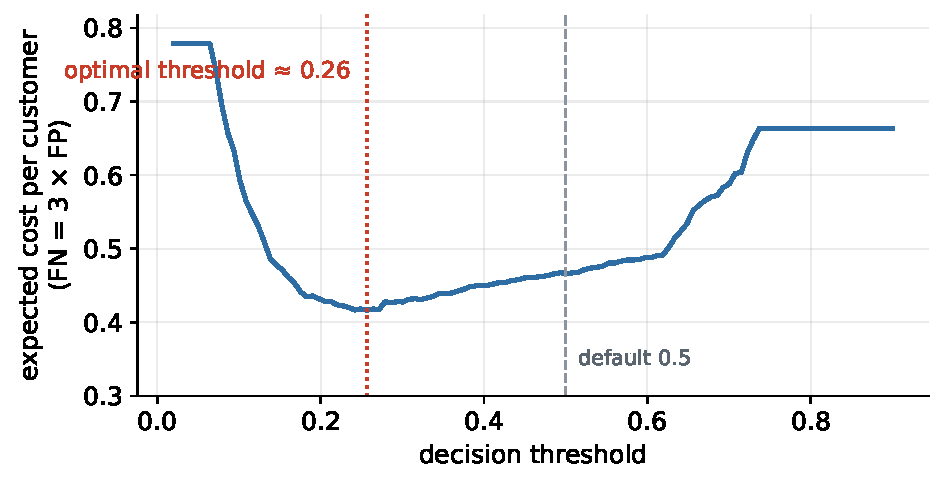
\includegraphics[width=0.58\textwidth]{lecture_3/figures/fig_expected_cost.pdf}
\caption{Expected cost against the threshold: the optimum is a business
number, not 0.5.}
\label{fig:cost3}
\end{figure}

\subsection{Leakage: the detonation}
\texttt{collections\_contact} has been in the portfolio since Block 1,
flagged \emph{do not use}: collections calls customers mostly \emph{after}
they default, so at application time the value does not exist. Adding this
single column to the tuned GBDT lifts test AUC from 0.773 to
\textbf{0.953} (Figure~\ref{fig:leak3}) - the best model this course will
ever produce, and completely worthless, because the feature is unknowable
at decision time.

\begin{figure}[htbp]
\centering
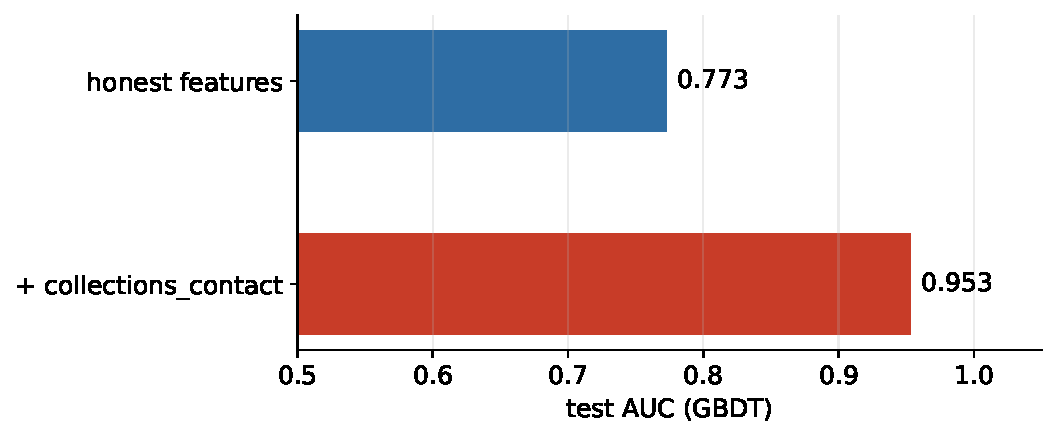
\includegraphics[width=0.62\textwidth]{lecture_3/figures/fig_leakage.pdf}
\caption{One added column: the leakage detonation.}
\label{fig:leak3}
\end{figure}

What makes leakage dangerous is its seductiveness. The leaky feature looks
like your best feature - importance rankings crown it instantly. Every
honest-looking check passes: cross-validation loves it and the test set
loves it, because the leak sits on both sides of every split. Nothing
crashes and no warning fires; the only failing dataset is the one you do
not have yet, production. Leakage is therefore caught by \emph{reasoning
about features}, not by metrics - the metrics are its accomplices.
Sit with that last sentence, because it inverts everything this
chapter built. The entire evaluation apparatus - CV spreads, held-out
tests, honest protocols - assumes the future will resemble the data
you evaluated on. Leakage breaks that assumption at the level of a
single column: the evaluation data contains information the production
data will not, so every metric computed on it, however carefully, is
measuring the wrong world. This is why an evaluation section and a
leakage section belong in the same block - the second is the failure
mode of the first.

\subsubsection{A taxonomy of leaks}
The bestiary organises into four families, and naming the family is
half the diagnosis. \emph{Target leakage}: a feature that encodes the
outcome itself - post-outcome fields (\texttt{collections\_contact},
\texttt{account\_closed\_reason}) recorded because the default already
happened, and target twins (\texttt{months\_overdue} predicting
default) that are near-definitions of the label. These are the
loudest leaks: one column, spectacular scores, and the time-travel
question kills them instantly once it is asked. \emph{Train-test
contamination}: information crossing the split through the procedure
rather than through any single column - transform leaks (scaler,
imputer or encoder fitted on all data before splitting; the CV-hygiene
example above), and duplicate leaks (the same customer, or the same
row after a join gone wrong, appearing in train and test so the model
is quizzed on questions it has memorised). \emph{Temporal leakage}:
the future informing the past - time-travel joins (feature tables
joined from post-decision snapshots, so ``income'' is the value known
a year after the decision, not at it), and random splits on drifting
data that let the model train on customers from after the test
window. \emph{Group leakage}: rows that belong together split apart -
one person's several loans divided across sides, so the ``unseen''
test loan shares its owner with a training loan; households, branches
and merchants leak the same way. The last three families are the
sneaky ones - no single column looks guilty; the \emph{procedure}
leaks - and they are caught by auditing the split and the joins, not
the feature list.

\subsubsection{The time-travel test as an audit protocol}
The smells that should trigger an audit: AUC far above the domain's normal
range, one feature dominating importance, test far above CV. Any one of
the three is enough to stop; two together are close to proof. The
audit itself should be boringly systematic - a protocol, not a
vibe. For every feature, write down the answer to one question:
\emph{at the moment the decision would be made, is this value already
in the database?} - not ``does the column exist'', but whether the
\emph{value} for this customer, at this timestamp, could have been
queried. Record the answer per feature, with the source system and the
snapshot date of the table it came from; a feature nobody can answer
for is treated as leaky until proven otherwise. Then audit the
procedure: confirm every join uses a snapshot dated before the
decision; check identifier keys for duplicates across the split;
confirm rows sharing a customer, household or contract sit on the same
side; and if time exists in the data, demand the out-of-time test,
because it is the one evaluation design that catches temporal leaks
mechanically - a feature computed from the future cannot help on a
test window that lies beyond the training period's future. The
checklist before believing any good result compresses to four lines:
every feature has a written answer to
``when is this value known?''; all transforms live inside the pipeline;
keys are checked and groups split together; and if time exists in the data,
an out-of-time test exists too. Teams that run this protocol routinely
treat a surprisingly good number the way an engineer treats a
surprisingly quiet engine - as a symptom, first.

\subsection{Explaining models}
Two standard answers to ``which features matter?''
(Figure~\ref{fig:imp3}): \emph{impurity importance} - how much Gini each
feature removed - is free and train-side, but biased (it loves
high-cardinality features and splits credit among correlated ones);
\emph{permutation importance} shuffles one column on the \emph{test set}
and measures the AUC drop - slower, model-agnostic, honest about what the
model actually uses.

\begin{figure}[htbp]
\centering
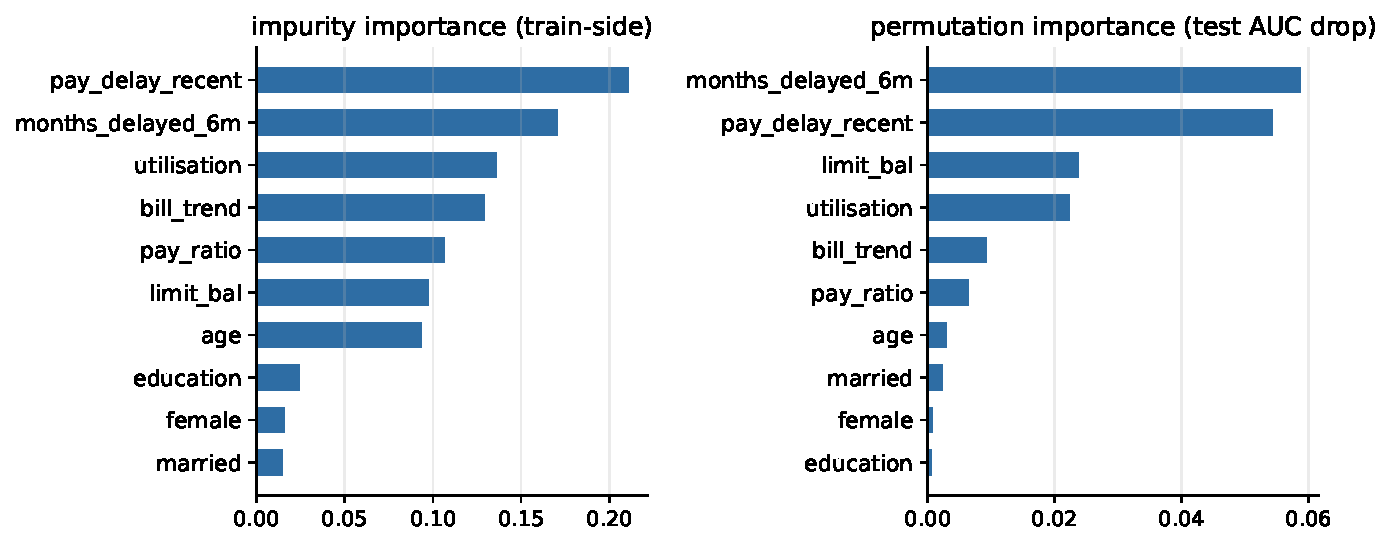
\includegraphics[width=0.85\textwidth]{lecture_3/figures/fig_importance.pdf}
\caption{Impurity versus permutation importance for the forest.}
\label{fig:imp3}
\end{figure}

\subsubsection{Permutation importance: mechanics and failure modes}
The mechanics are almost embarrassingly simple, which is their virtue.
Score the model on the test set. Take one column, shuffle its values
across rows - destroying its relationship to the outcome while
preserving its marginal distribution - and score again. The drop in
AUC is that feature's importance: how much the model's performance
\emph{depended} on that column carrying real information. Repeat the
shuffle several times and average, because one permutation is one
random draw; features the model ignores show drops near zero, and the
whole procedure needs nothing from the model but predictions - it
works identically for a forest, a GBDT, or next block's neural
network.

Its honest failure mode is correlated features, and it fails in both
directions at once. Direction one, \emph{understatement}: if
utilisation has a near-twin (say, balance-to-limit computed slightly
differently), shuffling one leaves the model leaning on the other, the
AUC barely drops, and \emph{both} twins can report near-zero
importance while being jointly indispensable - the same
credit-splitting pathology as Block 2's lasso choosing one twin.
Direction two, \emph{distortion}: shuffling breaks the correlation
structure itself, so the model is evaluated on impossible customers -
high utilisation paired with the twin's low value, combinations that
never occur - and its behaviour off the data manifold is being
measured, not its behaviour in reality. Neither failure makes the tool
useless; both mean a permutation ranking is read alongside a
correlation matrix, and features are shuffled in correlated
\emph{groups} when the question is ``does this cluster of information
matter'', not ``does this exact column''.

Impurity importance's bias also has a mechanism worth knowing rather
than memorising. A feature with many distinct values offers many
candidate cut-points, hence many chances to find a split that fits
noise - so high-cardinality features accumulate impurity credit they
have not earned. And because the score is computed on the training
data, splits that merely memorised are counted as contributions.
Free is the right price for it: use impurity importance as a quick
first look, and permutation on held-out data for anything anyone will
act on.

\subsubsection{SHAP, in one honest paragraph}
\textbf{SHAP} generalises Block 2's receipt: for one
prediction, attribute the deviation from the average outcome across
features fairly (Shapley values); locally it yields one customer's bars
(adverse-action material), globally an importance ranking with direction.
The fairness has a precise meaning imported from game theory: each
feature's credit is its average marginal contribution over all orders
in which features could be revealed, and the attributions provably sum
to the gap between this customer's prediction and the average one -
the receipt always adds up. For tree ensembles the computation is
exact and fast (TreeSHAP); for arbitrary models it is approximated by
sampling.
Its costs: computation, and ambiguous credit-sharing among correlated
features - the same twins that confuse permutation importance confuse
Shapley attribution, and no amount of game theory can decide which of
two interchangeable columns ``really'' did the work. Students who understood the logistic decomposition already know
what a SHAP plot is trying to be: the coefficients-times-values
receipt, rebuilt for models that have no coefficients.

\subsubsection{Monotonic constraints: domain knowledge as a leash}
Domain knowledge can also enter as a constraint: modern GBDT accepts
\emph{monotonic constraints} (\texttt{monotonic\_cst}), forcing the score
non-decreasing in chosen features - regularisation, explainability and
regulator comfort in one move; risk that locally \emph{falls} as
utilisation rises is an artefact nobody should have to defend. The
constraint is a leash in the exact technical sense of this course: it
shrinks the space of functions the ensemble may fit, trading a little
flexibility for stability - and when the constraint encodes something
true about the world, the trade is nearly free, because the wiggles it
forbids were noise. It is the same move as Block 1's binning and
Block 2's chosen coefficients: domain knowledge entering the model on
purpose, in a form an auditor can read.

And one
boundary to keep sacred: explanations explain \emph{the model}, not the
world. Importance is not causality; correlated features trade places
between runs (remember lasso picking one twin). Utilisation
``mattering'' means the model leans on it, not that persuading
customers to reduce utilisation would lower their risk - the feature
may simply be the visible shadow of something else. Legitimate uses are
debugging (a dominant weird feature is a leakage smell - importance
rankings are the leak-detector this block already used once),
monitoring (importance drift as an early warning that the portfolio is
changing under the model), and communication - with the caveats spoken
aloud. Policy conclusions need causal designs, which lie beyond this course but
not beyond your career.

\subsection{Lab and hand-in}
The lab notebook \texttt{03\_trees\_ensembles\_evaluation} runs the whole
arc: cross-validating the Block 2 baseline (fold spread first); growing,
reading and leashing a tree (whose root split agrees with the logistic
coefficients); the four-model tournament under one CV protocol; ROC, PR and
calibration for the finalists; the leakage detonation with permutation
importance crowning the leak; and the expected-cost sweep that moves the
threshold from 0.5 to $\sim$0.26 for a $\sim$11\% saving. Exercises add raw
NaNs fed natively to HistGBDT, a forest leash sweep, isotonic calibration,
a cost-ratio sensitivity analysis, and an optional monotonic constraint.
``Done'' means being able to say which model won, whether the gap beats the
CV spread, and at which threshold you would run it - with a cost curve to
back you up. Project checkpoint: teams are final, and the rubric's
evaluation criterion (20\%, ``correct, leakage-aware'') now has an
operational definition - the minimum kit is CV mean $\pm$ sd, ROC
\emph{and} PR, a calibration look, one cost-based threshold argument, and a
written time-travel audit of the features. That kit, executed cleanly,
is most of the difference between a passing project and a memorable
one - and it is, feature for feature, the same kit a validation team
would demand of a production PD model, which is not a coincidence.

% =====================================================================
\section{Block 4 - Clustering \& dimensionality reduction}

Blocks 2 and 3 had a luxury we now lose: a label. Without
\texttt{default} to predict, there is no ground truth, no test set that can
say ``correct'', and no error with a price. The goal becomes
\emph{structure} - groups of similar customers, compressed
representations - and the standard of judgement becomes usefulness,
which is argued rather than measured. One consequence deserves to be
stated before any algorithm: an unsupervised method \emph{always returns
an answer}, and nothing in the mathematics says whether the answer means
anything. Ask k-means for four clusters and you will receive four
clusters - on your portfolio, on a table of random numbers, on the
digits of $\pi$. The supervised world had a built-in humiliation
mechanism - a model that learned nothing scored an AUC of 0.5, and the
test set said so in public; that mechanism is gone. Scepticism
graduates from a virtue to a method.

Why does a lender cluster at all? Customer segmentation feeds strategy,
product design and communication - ``who are our customers, in four
sentences?'' is a question every retail bank asks and clustering is the
disciplined way to answer it. Anomaly detection - customers unlike
everyone else - feeds fraud work and data-quality checks; it is Block
1's outlier perspective upgraded from cleaning chore to deliverable.
Clusters are EDA power tools, hypotheses about heterogeneity you did not
know to look for. And compression (PCA) turns dozens of correlated
features into a few components. What clustering is \emph{not} for, in a
regulated shop, is making individual credit decisions: segments inform
strategy; the PD model prices the person. The workflow is a recipe with
five steps - representation, distance, algorithm, validation, naming
- and, as always in this course, the early steps decide more than the
algorithm: by the time you have chosen which features describe a
customer and what ``similar'' means numerically, most of the answer is
already fixed, and the algorithm merely reads it out.

\subsection{Working without ground truth}
With no ground truth, evaluation rests on a triad: \emph{internal
metrics} (inertia, silhouette - necessary, never sufficient),
\emph{stability} (reseeding, resampling, next quarter - the
unsupervised cousin of cross-validation), and \emph{external usefulness}
(profiles against outcomes held out of the clustering, plus the business
sniff test). Each leg deserves honest scrutiny, because each can be
fooled - and a practitioner who knows how each substitute fails is
much harder to mislead.

Internal metrics measure geometry, not meaning. A silhouette score asks
whether points sit closer to their own cluster than to the next one -
a sensible question, but one posed entirely inside the feature space
you built: if that space encodes an artefact (an unscaled income
column, a duplicated concept), the metric happily certifies the
artefact. Worse, every internal index carries its own aesthetic -
silhouette and inertia both prefer round, compact, well-separated
blobs, structurally biased towards the kind of answer k-means produces.
Using inertia to validate k-means is close to letting the student grade
their own exam: useful for comparing runs, never proof of truth.

Stability is a stronger substitute because it asks a falsifiable
question: if the data had come out slightly differently - another
random start, another 80\% subsample, next quarter's snapshot - would
we have told the same story? Structure that evaporates under reseeding
was never structure. But stability is necessary, not sufficient: a
perfectly stable answer can be a perfectly stable artefact. Cluster on
raw, unscaled incomes and you will get the same income bands every time
- stable, reproducible, and meaningless as a statement about customer
behaviour.

External usefulness is the strongest leg: hold an outcome \emph{out} of
the clustering - default, churn, profitability - then check whether
the segments separate on it. If groups built purely from behaviour turn
out to have default rates ranging from 15\% to 58\%, the structure has
demonstrated cash value on information it never saw. Even this test has
a limit worth naming: it validates the segmentation \emph{for that
outcome} - a segmentation useless for credit risk might be excellent
for marketing, and vice versa. ``Is this clustering good?'' is not a
well-posed question; ``is this clustering good \emph{for this
decision}?'' is. Keep the triad in mind through the whole chapter -
every method we meet will be judged by it.

\subsection{Distance, scaling, and the curse}
Distance is a modelling choice. Euclidean distance
$\sqrt{\sum_j (x_{aj}-x_{bj})^2}$ is the default and, through its squares,
amplifies large single-feature gaps; Manhattan distance sums absolute
gaps and forgives an extreme coordinate; cosine similarity (angle, not
length) waits for text in Block 5; mixed numeric and categorical data
needs care (Gower's coefficient is the classical fix). A small worked
example makes the units concrete: two customers standing $1.0$, $-1.2$
and $-0.2$ standard deviations apart on three standardised features are
$\sqrt{2.48} \approx 1.57$ apart in Euclidean terms - about one and a
half ``typical spreads'' - and $2.4$ in Manhattan terms.

\subsubsection{A menu of distances, and what each one rewards}
Stay with that worked pair, because it already exposes the character of
the two metrics. The three per-feature gaps are $1.0$, $1.2$ and $0.2$.
Under Manhattan, each contributes in proportion:
$1.0 + 1.2 + 0.2 = 2.4$, and the small age gap supplies about 8\% of
the total. Under Euclidean, the gaps are squared first:
$1.00 + 1.44 + 0.04 = 2.48$, and the age gap's share collapses to under
2\% - squaring is a megaphone for the largest disagreement. If you
believe one extreme coordinate should be able to dominate ``similar''
- a customer four months delinquent is simply different, whatever else
matches - Euclidean encodes that belief; if you want ten small
disagreements to weigh the same as one large one, Manhattan does. There
is no correct answer - only the answer you chose, whether or not you
noticed choosing.

Cosine distance drops magnitude entirely and compares direction. Take
two customers whose monthly spending across two categories is $(2, 4)$
and $(1, 2)$: Euclidean sees a gap of $\sqrt{1^2 + 2^2} \approx 2.24$,
while cosine sees two vectors pointing the same way - proportionally
identical spenders, one simply operating at twice the scale - and
reports a distance of zero. Exactly right for documents (Block 5),
where long and short articles on one topic should count as similar;
for balances, perhaps not - which is the point.

Mixed data breaks all three: what is the ``distance'' between renting
and owning? Gower's coefficient handles each feature in its own
currency and averages: numeric features contribute their absolute gap
divided by the feature's range (landing in $[0,1]$), categorical
features contribute $0$ for a match and $1$ for a mismatch. A
micro-example: limits of 60k and 160k on a portfolio spanning 500k give
$100/500 = 0.20$; housing \texttt{rent} versus \texttt{rent} gives $0$;
ages 30 and 40 on a 50-year range give $10/50 = 0.20$; Gower distance
$(0.20 + 0 + 0.20)/3 \approx 0.13$. Not exam material, but the design
lesson is: someone must decide how a category mismatch trades against a
numeric gap, and if you do not decide, the encoding decides for you.

The feature list itself is the definition of ``similar'': every column is
one vote. Application-time information only (segments built on
post-outcome fields inherit every leakage pathology of Block 3); one
concept, one vote (two utilisation variants let utilisation vote twice);
business-relevant only (identifiers never - \texttt{customer\_id} would
vote that consecutively onboarded customers are alike - and
near-constant columns never, since they vote ``everyone is similar'');
and the target stays out - \texttt{default} is reserved for
\emph{profiling}, because clustering on it manufactures fake foresight.

\begin{figure}[htbp]
\centering
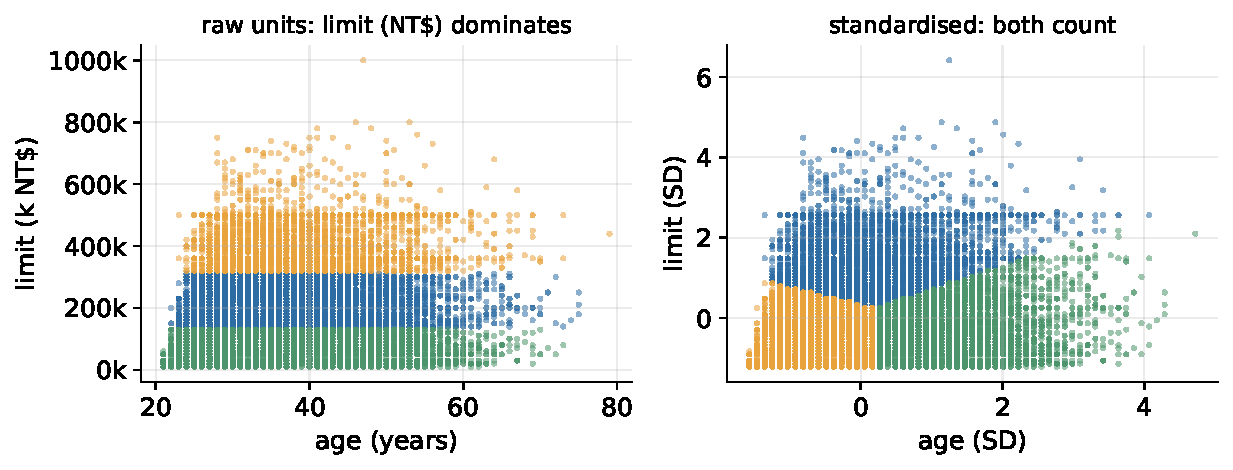
\includegraphics[width=0.8\textwidth]{lecture_4/figures/fig_scaling_matters.pdf}
\caption{The same two features, clustered raw and standardised. In raw
units, income is the only voter.}
\label{fig:scale4}
\end{figure}

\subsubsection{Why scaling changes the answer}
Scaling, optional for trees, is \emph{never} optional for distances:
Figure~\ref{fig:scale4} shows k-means on raw units producing pure income
bands - age never got a vote. The arithmetic behind the figure is
worth doing once by hand. Take two customers: incomes 120{,}000 and
80{,}000 PLN, ages 25 and 60. In raw units the Euclidean distance is
\[
  \sqrt{40{,}000^2 + 35^2} \approx 40{,}000.02 :
\]
a 35-year age gap - practically a different generation - moves the
distance by two hundredths of one income unit. The metric is not
weighing the features; the units are. Now standardise. If income has a
standard deviation of roughly 40{,}000 PLN and age of roughly 12 years,
the gaps become $1.0$ and $2.9$ standard deviations, and the distance is
$\sqrt{1.0 + 8.5} \approx 3.1$ - suddenly age dominates, because in
``how unusual is this gap among customers?'' terms, 35 years is the
bigger disagreement. Neither number is wrong; they answer different
questions; standardising answers the one you almost always mean -
distances in units of typical customer-to-customer spread, one vote per
concept. Trees forgave you this (splits are order-based); distances
never will.

\subsubsection{The curse of dimensionality}
Finally, the \emph{curse of dimensionality}: as dimensions grow,
distances concentrate until the nearest and farthest customers are
nearly equally far. The intuition is additive noise. Every feature
contributes one term to the sum of squared gaps; if the features are
mostly unrelated, those terms average out, and the total distance
between two random customers hugs its expected value ever more tightly
- the sum grows like the number of dimensions $d$, while its spread
grows only like $\sqrt{d}$, so the \emph{relative} spread shrinks like
$1/\sqrt{d}$.

A numeric illustration makes it vivid. Scatter points uniformly in the
unit cube $[0,1]^d$ and measure the distance between two random points:
the typical distance is about $\sqrt{d/6}$, while its standard deviation
stays near $0.24$ \emph{regardless of} $d$. In $d = 6$ dimensions (our
six clustering features), that is a typical distance of about $1.0$
with a spread of $0.24$ - distances vary by a quarter of their size,
and ``near'' versus ``far'' still means something. In $d = 100$, the
typical distance is about $4.1$ with the same spread - a 6\% relative
variation; in $d = 1000$, under 2\%. Every customer becomes
approximately equally far from every other, and any algorithm built on
``who is close?'' is asking a question the geometry can no longer
answer. Practical consequences: cluster on a curated feature set, not on
everything you have; watch for correlated double-counting; and treat
dimensionality reduction - PCA, later this chapter - as a legitimate
opening move rather than an afterthought.

\subsection{K-means}
K-means is one loop (Figure~\ref{fig:kmsteps4}): pick $k$ centres; assign
every point to its nearest centre; move each centre to its points' mean;
repeat until nothing changes. It minimises the within-cluster sum of
squares (``inertia''),
\[
  \min_{\text{assignments}}\;
  \sum_{k=1}^{K} \sum_{i \in C_k} \lVert x_i - \mu_k \rVert^2 ,
\]
which bakes in assumptions - clusters roughly round, similar in size
and spread, in the \emph{scaled} space - and carves the feature space
into convex cells around the centroids.

\begin{figure}[htbp]
\centering
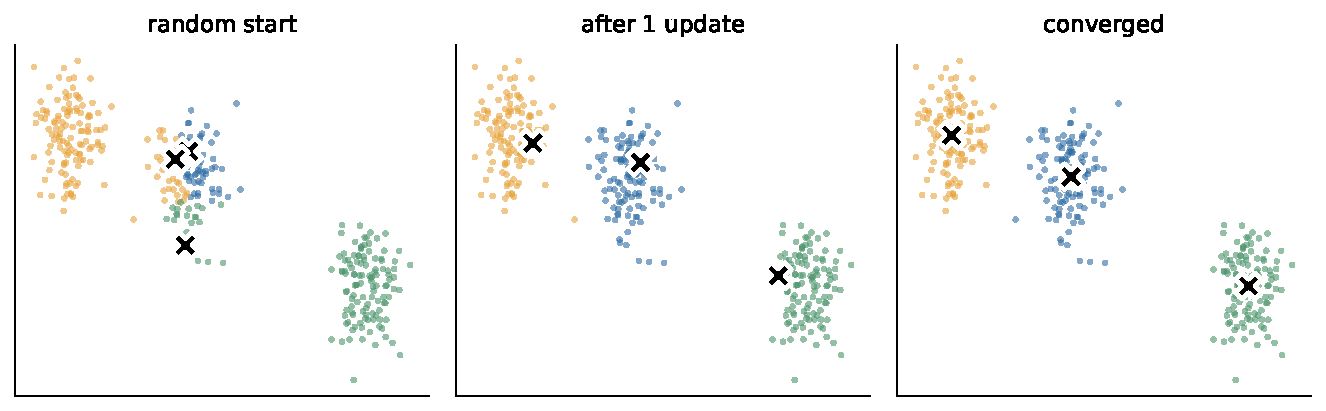
\includegraphics[width=0.86\textwidth]{lecture_4/figures/fig_kmeans_steps.pdf}
\caption{K-means: assign, update, repeat.}
\label{fig:kmsteps4}
\end{figure}

\subsubsection{Lloyd's algorithm: why it always converges, and why only locally}
The loop above is Lloyd's algorithm, and it is worth seeing as
\emph{coordinate descent} on the inertia: the objective has two blocks
of unknowns - the assignments and the centres - and each step
optimises one block exactly while holding the other fixed. The
assignment step cannot increase inertia: moving a customer to a nearer
centre only shrinks their squared-distance term. The update step cannot
increase it either, by a one-line calculus fact: among all candidate
centre positions, the arithmetic mean minimises the sum of squared
distances to a fixed set of points. So inertia falls (or stays put) at
every step; since there are finitely many ways to partition $n$
customers into $k$ groups, a quantity that never increases must
eventually stop changing - convergence is guaranteed, typically
within a handful of iterations.

What is \emph{not} guaranteed is convergence to the best answer.
Coordinate descent stops at the first configuration where neither block
can improve alone, and such local optima can be badly wrong. A toy you
can verify by hand: four customers at the corners of a long rectangle,
$(0,0)$, $(0,1)$, $(4,0)$, $(4,1)$, with $k = 2$. The right answer
pairs the nearby corners - left pair and right pair - for an inertia
of $4 \times 0.5^2 = 1$. But start the centres at $(2,0)$ and $(2,1)$
and k-means pairs the \emph{bottom} corners against the \emph{top}:
each point sits distance $2$ from its own centre and
$\sqrt{5} \approx 2.24$ from the other, so no point wants to switch, no
centre wants to move, and the algorithm halts - contentedly - at
inertia $16$, sixteen times worse than the optimum, with nothing in the
output to warn you. This is why the start matters, and why two cheap
insurance policies are standard practice.

The first is smarter seeding: \emph{k-means++} picks the first centre
at random, then picks each subsequent centre with probability
proportional to the squared distance from the nearest centre already
chosen. Far-flung regions - exactly the ones a uniform random start
tends to miss - get proportionally more chance to host a centre, so
the initial centres arrive spread out rather than huddled in one dense
area. The second is repetition: \texttt{n\_init=10} runs the whole
algorithm from ten starts and keeps the partition with the lowest
inertia - internal metrics used exactly as intended, to compare runs
of the same method, not to certify truth. Together they make the
rectangle pathology rare, though never impossible; and since the final
partition still depends on the seed, \texttt{random\_state} is part of
the segmentation's recipe - Block 1's reproducibility rule,
unsupervised edition. Two smaller practical notes: squared distances
chase outliers, so inspect (or winsorise) extreme customers first, or
use k-medoids, the robust cousin that centres on actual customers; and
k-means is fast enough for millions of rows, with
\texttt{MiniBatchKMeans} buying another order of magnitude of scale for
a small quality discount.

\begin{figure}[htbp]
\centering
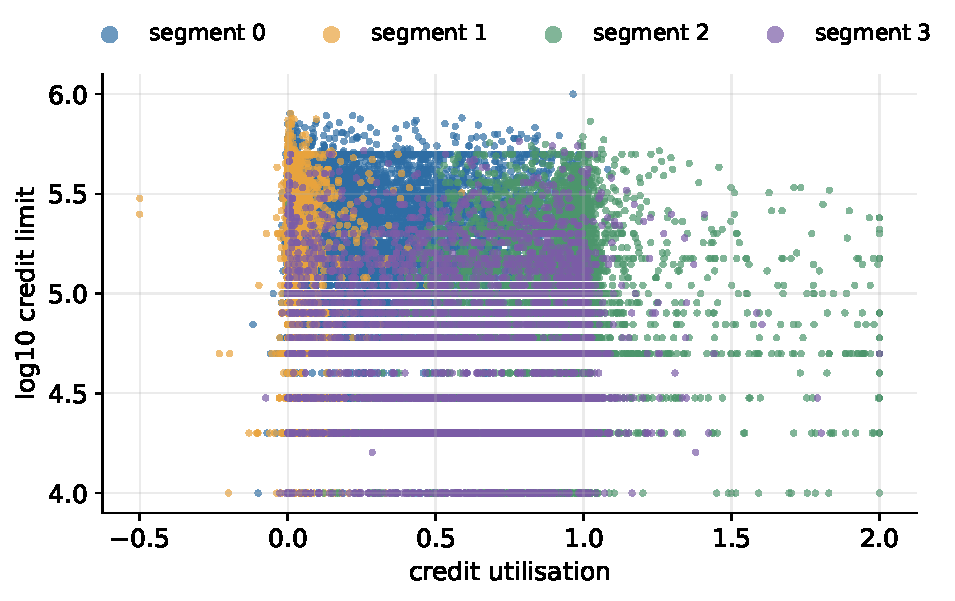
\includegraphics[width=0.58\textwidth]{lecture_4/figures/fig_kmeans_portfolio.pdf}
\caption{$k=4$ on six scaled features, shadowed onto two of them. The wall
at zero utilisation is the transactor population.}
\label{fig:kmport4}
\end{figure}

On the portfolio we cluster on six scaled behavioural features - log
limit, age, utilisation, months delayed, payment ratio, bill trend - with
the target excluded, and sex and marriage excluded too: protected traits
must not define ``similar'', even in strategy work
(Figure~\ref{fig:kmport4}). Even the raw scatter teaches: the dense wall
of points at utilisation near zero is the transactor population - clients
who pay in full every month - visible before any algorithm runs.

\begin{figure}[htbp]
\centering
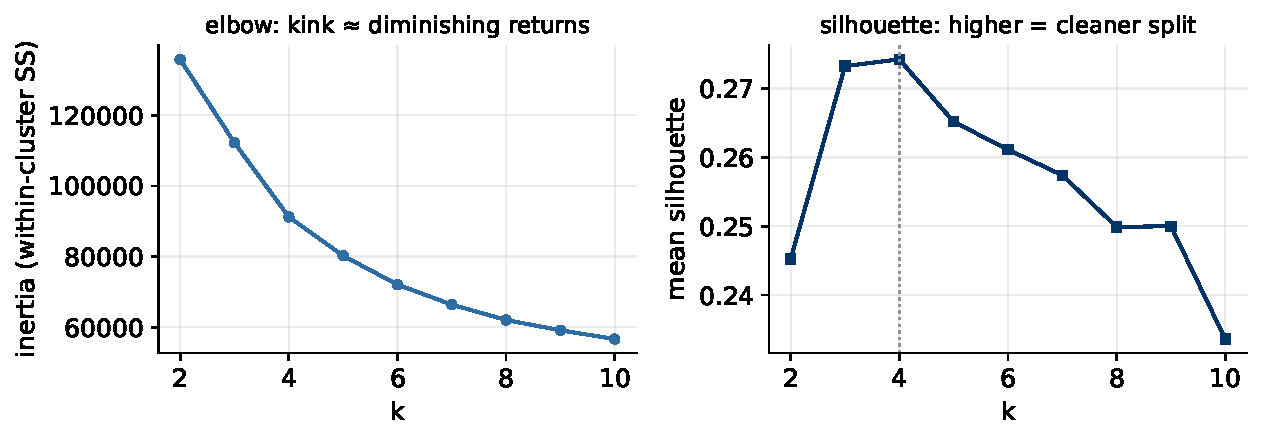
\includegraphics[width=0.86\textwidth]{lecture_4/figures/fig_elbow_silhouette.pdf}
\caption{Choosing $k$: inertia (elbow) and mean silhouette.}
\label{fig:elbow4}
\end{figure}

\subsubsection{Choosing $k$: the elbow's logic}
Choosing $k$ (Figure~\ref{fig:elbow4}) starts from a fact about
inertia: it \emph{always} falls as $k$ grows. Adding a centre can only
help - at worst it sits unused - and at $k = n$ every customer is
their own centre and inertia is zero. So the raw value of inertia at
any single $k$ proves nothing; what carries information is the
\emph{shape} of the curve. If the data genuinely contains four groups,
moving from $k = 3$ to $k = 4$ lets the centres finally cover all of
them and inertia drops sharply; moving from $k = 4$ to $k = 5$ merely
splits a real group in two and buys little. The \emph{elbow} is that
kink of diminishing returns - the point where extra centres stop
paying for themselves. On our portfolio the curve is smooth, with no
clear kink: the honest reading of an elbow plot is often ``the data
declines to commit'', and that non-answer is itself information about
how firm the structure is.

\subsubsection{The silhouette, worked by hand}
The \emph{silhouette} gives each individual customer a verdict. For
customer $i$, let $a_i$ be the mean distance from $i$ to the other
members of its \emph{own} cluster (cohesion: how far is home?), and
$b_i$ the mean distance from $i$ to the members of the \emph{nearest
other} cluster (separation: how far is the best alternative?). Then
\[
  s_i = \frac{b_i - a_i}{\max(a_i, b_i)} ,
\]
which lands in $[-1, 1]$: positive when home is closer than the
alternative, zero on the fence, negative when the customer actually
sits nearer to a neighbouring cluster than to their own. Three worked
cases pin down the scale. A customer with $a_i = 0.4$ and $b_i = 1.6$
scores $s_i = 1.2/1.6 = 0.75$ - home is four times closer than the
alternative; this customer is deep inside their cluster. A customer
with $a_i = 1.0$ and $b_i = 1.1$ scores $s_i = 0.1/1.1 = 0.09$ - the
two clusters are nearly equally plausible; this customer sits on a
border, and the hard assignment k-means reports is close to a coin
flip. And a customer with $a_i = 1.5$ and $b_i = 0.9$ scores
$s_i = -0.6/1.5 = -0.40$ - the ``nearest other'' cluster is actually
closer than home; this customer is probably mis-assigned, a casualty of
convex cells or a bad local optimum. Averaging $s_i$ over all customers
gives the mean silhouette - the single number on the right panel of
Figure~\ref{fig:elbow4}.

Ours peaks exactly at our $k=4$, at $0.27$ - moderate, genuine
grouping: the transactor wall and the delinquent tail are real
behavioural islands, though the groups touch and many clients live near
a border. After the worked cases, $0.27$ has a face - most customers
clearly closer to home, mixed with a genuine borderland of near-zero
scores. The contrast with Block 1's synthetic portfolio is the teaching
point: there the same diagnostic read 0.12 - one connected cloud -
and k-means returned four sharp segments anyway. The number, not the
picture, tells you how much to believe; the report sentence - state
$k$, the silhouette, and how firm the borders are - belongs in every
segmentation deliverable either way. (Remember, though, that the
silhouette shares k-means' taste for round, separated blobs - a second
witness, not an independent judge.) Where k-means breaks structurally
- stretched clusters, unequal spreads (Figure~\ref{fig:kmfail4}) -
the centroids land wrong \emph{confidently}; when the shapes are wrong
for the tool, change the tool.

\begin{figure}[htbp]
\centering
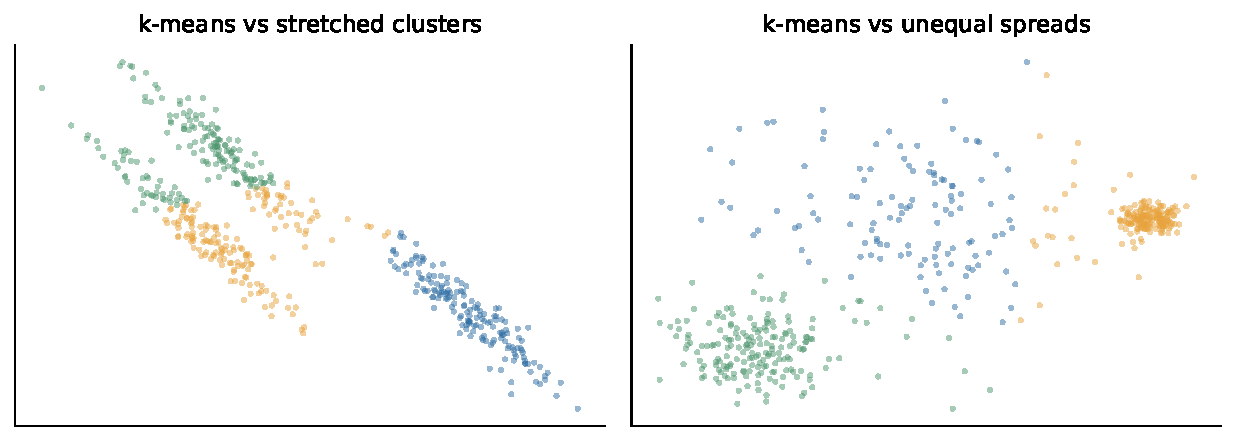
\includegraphics[width=0.78\textwidth]{lecture_4/figures/fig_kmeans_fails.pdf}
\caption{K-means versus shapes that violate its assumptions.}
\label{fig:kmfail4}
\end{figure}

\subsection{Hierarchies and density}
\emph{Agglomerative clustering} starts with every customer alone and
repeatedly merges the two closest clusters, recording the whole history.
``Closest between clusters'' is the linkage: single (nearest members -
chains), complete (farthest - compact, brittle), average, or Ward
(least variance increase - k-means' cousin and the usual default). The
cost is pairwise distances: fine for thousands, painful for millions -
sample first.

\subsubsection{Linkage: four definitions of ``close'', four personalities}
The linkage choice deserves more than a list, because it changes what
the method can find. \emph{Single linkage} calls two clusters close if
their \emph{nearest} members are close. That lets clusters grow by
touching - a chain of customers, each near the next, merges into one
long snake even if its ends are far apart: a gift when the true
structure is elongated, a disease otherwise, since one noisy customer
sitting between two genuine groups becomes a bridge and the groups
merge through it. \emph{Complete linkage} is the opposite temperament:
two clusters are only as close as their \emph{farthest} members, so a
cluster cannot absorb anything that would stretch its diameter -
compact, round groups, but brittle, because a single outlier on a
cluster's rim inflates its apparent distance to everything.
\emph{Average linkage} splits the difference. \emph{Ward's method}
merges whichever pair increases total within-cluster variance the least
- greedily optimising a hierarchical version of k-means' inertia,
which is why it shares k-means' preference for similarly sized round
groups and why it is the usual default for customer work. The trade-off
in one sentence: single linkage risks chaining, complete and Ward risk
shattering elongated shapes; you are choosing which mistake you would
rather make.

\subsubsection{Reading a dendrogram}
Agglomerative clustering's gift is the \emph{dendrogram}
(Figure~\ref{fig:dendro4}): the whole merge history in one picture,
with each merge drawn at a height equal to the distance at which it
happened. Read it vertically: long vertical runs mean a group survived
a wide range of distances without being forced to merge - genuine
separation - while short runs mean the merge order was nearly
arbitrary. To extract a flat clustering, cut horizontally where the
vertical runs are long, and the number of branches you sever is your
$k$: one picture holds every $k$ at once. Ours merges early and often
- the weak-structure verdict from a second witness. Sometimes, though,
the hierarchy itself is the deliverable: strategy wants five coarse
super-segments, CRM wants twenty fine ones, and a dendrogram serves
both from one fitted object, with the guarantee that the fine
segmentation nests cleanly inside the coarse one - something two
separate k-means runs cannot promise.

\begin{figure}[htbp]
\centering
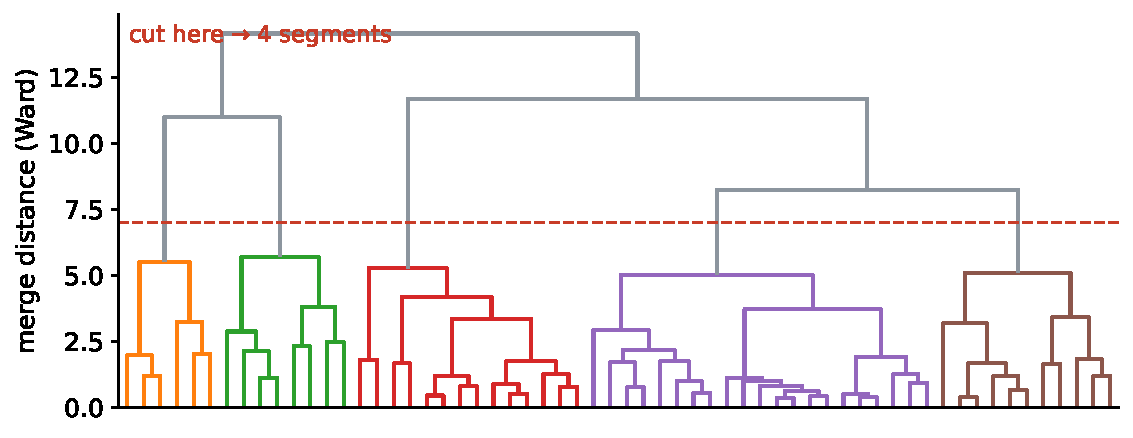
\includegraphics[width=0.8\textwidth]{lecture_4/figures/fig_dendrogram.pdf}
\caption{Ward dendrogram on a 60-customer sample.}
\label{fig:dendro4}
\end{figure}

\subsubsection{DBSCAN: clusters as dense places}
\emph{DBSCAN} abandons centres for density: a cluster is a packed region
- core points with at least \texttt{min\_samples} neighbours within
$\varepsilon$, plus their reachable friends - and everything else is
\textbf{noise}. The vocabulary is worth pinning down, because the
three-way point classification is the algorithm. A \emph{core point}
has at least \texttt{min\_samples} neighbours within radius
$\varepsilon$ - it sits in the thick of things, and clusters grow
outward from core points by connecting any two that fall within
$\varepsilon$ of each other. A \emph{border point} is not dense enough
to be core itself but lies within $\varepsilon$ of one - the shoreline
of a cluster; it joins, but cannot extend the cluster further. A
\emph{noise point} is neither - too far from any dense region - and
is labelled as such rather than forced into the nearest group.

Three superpowers follow: any shape (clusters grow by local
connectivity, not proximity to a centre, so crescents and rings are no
obstacle), no $k$ to choose (the density structure decides how many
clusters exist), and an explicit outlier label (in fraud work the noise
bucket is sometimes the entire deliverable). The price: touchy knobs
and \emph{one global density} - a single $\varepsilon$ must serve the
whole space, so a portfolio holding one tight group and one
legitimate-but-diffuse group defeats every setting: an $\varepsilon$
small enough to keep the tight group tight declares the diffuse group
noise, and one large enough to hold the diffuse group together merges
everything else. Choosing $\varepsilon$ has its own elbow - sort every
point's distance to its $k$-th nearest neighbour (with
$k = \texttt{min\_samples}$) and cut at the knee, where the curve stops
falling through empty space and flattens into the typical
within-cluster spacing; the elbow-and-scree philosophy again, and the
same admission of judgement. If no knee exists, densities vary too much
for one global $\varepsilon$, and HDBSCAN is the keyword.
Figure~\ref{fig:moons4} shows the classic contrast: two crescents that
k-means must slice with a line (convex cells oblige) and DBSCAN traces
naturally, quarantining stragglers as noise. Crescents are rare in
credit; the lesson is general - \emph{the algorithm's assumptions
decide what it can find}.

\begin{figure}[htbp]
\centering
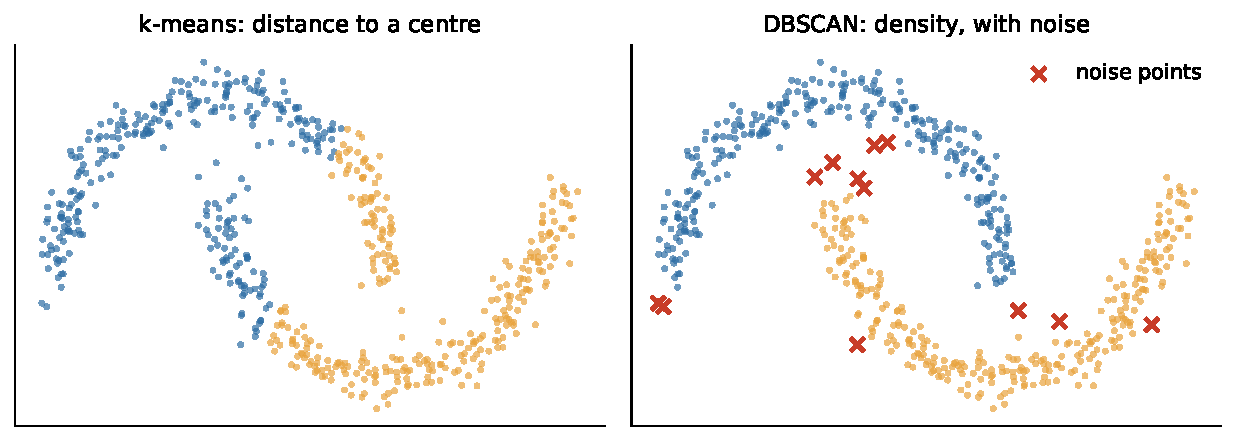
\includegraphics[width=0.78\textwidth]{lecture_4/figures/fig_dbscan_vs_kmeans.pdf}
\caption{Shapes k-means cannot see; DBSCAN's noise label at work.}
\label{fig:moons4}
\end{figure}

\subsubsection{Soft memberships: Gaussian mixtures in one honest paragraph}
Between the hard memberships of k-means and reality sit \emph{Gaussian
mixtures}: the data is modelled as a blend of $K$ Gaussian clouds, and
instead of answering ``which segment?'', the model answers ``with what
probabilities?'' - every customer gets a membership vector such as
70/25/5/0. The fitting algorithm, \emph{expectation-maximisation}
(EM), will feel familiar after Lloyd: the E-step computes each
customer's membership probabilities given the current clouds (the soft
analogue of the assignment step), and the M-step re-estimates each
cloud's centre, spread and weight as probability-weighted averages (the
soft analogue of the centroid update). Like Lloyd, every iteration
provably improves the objective - here, the likelihood - and like
Lloyd, EM converges only to a local optimum, so multiple starts remain
the insurance. K-means is exactly the hard-edged limiting case (round,
equal clouds, memberships forced to 0/1), and because a mixture is a
proper probability model, the number of components can be chosen by
BIC, the information-criterion cousin of the elbow. The honest caveat:
the clouds are still ellipses, so the model inherits a shape
assumption, and its probabilities are only as trustworthy as that
assumption. Credit likes mixtures anyway, for a credit-shaped reason:
borderline customers \emph{are} the interesting ones, and a 55/45
membership says ``borderline'' out loud where k-means would silently
pick a side.

\subsection{PCA}
Why compress? To \emph{see} (portfolios live in 20 dimensions; a faithful
2-D shadow beats twenty histograms), to fight the curse (fewer,
decorrelated dimensions make distances meaningful), to de-duplicate
(correlated features carry one concept several times), and to feed models
(components can replace dozens of raw features - at an
interpretability price). Principal component analysis finds the
directions of maximal variance: PC1 is the axis along which customers
differ most, PC2 the most-varying direction orthogonal to it, and so on
(Figure~\ref{fig:arrows4} shows income and savings collapsing onto a
shared ``affluence'' axis). Formally, PC1 solves
\[
  \max_{\lVert w \rVert = 1} \operatorname{Var}(Xw)
  = \max_{\lVert w \rVert = 1} w^{\top} \Sigma\, w
  \;\;\Longrightarrow\;\; \Sigma w = \lambda w :
\]
the components are the eigenvectors of the correlation matrix, ordered by
their eigenvalues - which \emph{are} the explained variances.
Components are orthogonal - multicollinearity dies here, delivering
Block 2's third remedy - and each is a \emph{recipe}: a weighted mix of
original features whose weights, the \textbf{loadings}, are the key to
interpretation.

\begin{figure}[htbp]
\centering
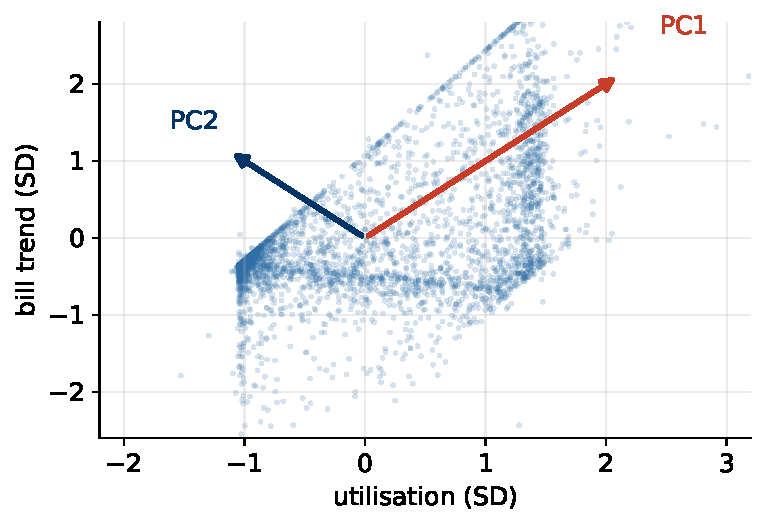
\includegraphics[width=0.44\textwidth]{lecture_4/figures/fig_pca_arrows.pdf}
\caption{PCA on two correlated features: the components are the cloud's
natural axes.}
\label{fig:arrows4}
\end{figure}

A two-feature toy shows the whole mechanism in miniature. Take two
standardised features with correlation $r$; their correlation matrix has
eigenvalues $1 + r$ and $1 - r$, so PC1 explains $(1+r)/2$ of the
variance. At $r = 0.8$ - income and savings, say - PC1 carries 90\%:
the cloud is a cigar, and one axis (the shared ``affluence'' direction)
tells most of the story. At $r = 0$ the eigenvalues are equal, the
cloud is round, and there is nothing to compress. The rule falls out
immediately: \emph{PCA's discount always equals the redundancy it finds
- no more, no less.}
One paragraph on computation, for honesty: in practice nobody forms
$\Sigma$ and calls an eigensolver; software factorises the centred data
matrix directly via the singular value decomposition,
$X = U S V^{\top}$, where the columns of $V$ are exactly the loading
vectors and the squared singular values, divided by $n - 1$, are
exactly the eigenvalues - same answer, better numerical behaviour, and
the reason sklearn's \texttt{PCA} mentions SVD in its documentation.

\begin{figure}[htbp]
\centering
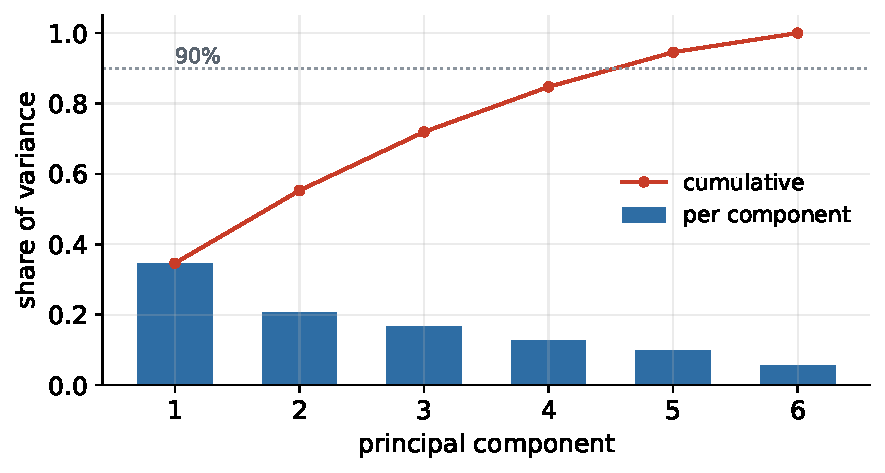
\includegraphics[width=0.6\textwidth]{lecture_4/figures/fig_scree.pdf}
\caption{Scree plot: little redundancy, little compression.}
\label{fig:scree4}
\end{figure}

How many components? The scree plot (Figure~\ref{fig:scree4}) answers:
PC1 explains 35\%, and 90\% takes five of six components - moderate
compression, tracking the correlation structure exactly. The bill-driven
features (utilisation, bill trend, payment ratio) share an axis; age
stands alone; PCA compresses redundancy, and here there is some - so
there is some discount. Reading a scree plot is the elbow skill again:
eigenvalues sorted in decreasing order, and you look for the drop after
which the remaining components are ``scree'' - the rubble at the foot
of a cliff, in the metaphor that named the plot. A steep-then-flat
profile says a few axes carry the story; our gentle slope says the six
features are genuinely six-ish concepts - itself a finding about the
feature set.

The loadings (Figure~\ref{fig:load4}) deliver the interpretation: PC1
loads positively on utilisation and bill trend and negatively on
payment ratio and limit - a \emph{revolving-stress axis}, nameable,
and a component nobody can name is a feature nobody can defend. Read a
loading vector exactly like a recipe: a customer's PC1 score is
(roughly) utilisation plus bill trend minus payment ratio minus log
limit, each in standardised units, so scoring high means heavily
utilised, bills growing, repaying small fractions, on a small limit.
Two honest footnotes belong next to any loadings chart. First,
\emph{signs are arbitrary}: if $w$ is an eigenvector then so is $-w$,
so a library update or a rerun on next quarter's data can flip every
sign on a component while changing nothing real. The \emph{axis} is
real; the direction is a labelling choice - fix a convention (``high
PC1 = high stress'') and state it, or two analysts will argue about a
minus sign that means nothing. Second, \emph{orthogonality has an
interpretive price}. Real behavioural constructs are correlated -
affluence and revolving stress genuinely co-move - but PCA forces
every component to be perpendicular to all previous ones, so PC2 is not
``the second most natural concept'' but ``the most-varying direction
\emph{after} PC1's shadow is removed''. Later components are
increasingly defined by what they must exclude, which is why PC1 and
PC2 usually earn clean names and PC5 rarely does.

\begin{figure}[htbp]
\centering
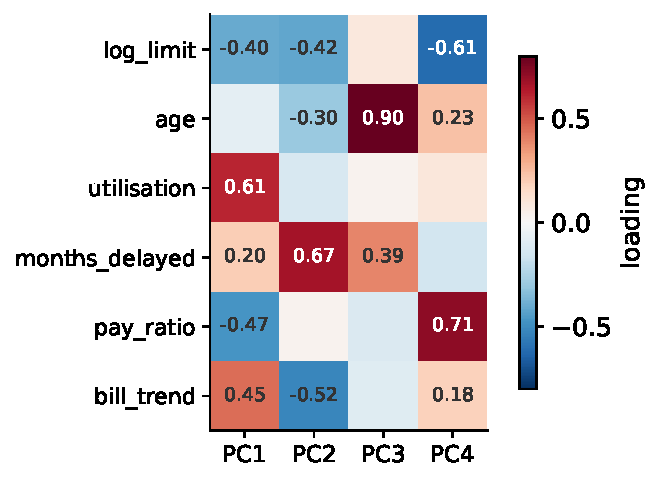
\includegraphics[width=0.5\textwidth]{lecture_4/figures/fig_loadings.pdf}
\caption{Loadings of the first four components.}
\label{fig:load4}
\end{figure}

An equivalent lens: keep $m$ components and \emph{reconstruct} - rebuild
each customer from their $m$ scores. The rebuild is imperfect, and the
reconstruction error equals exactly the variance thrown away, so
``explained 90\% with five components'' and ``reconstruction loses
10\%'' are the same sentence - use whichever the audience hears
better. This lens generalises: autoencoders (Block 6's cousins) are
this idea with nonlinear compress and decompress.

\begin{figure}[htbp]
\centering
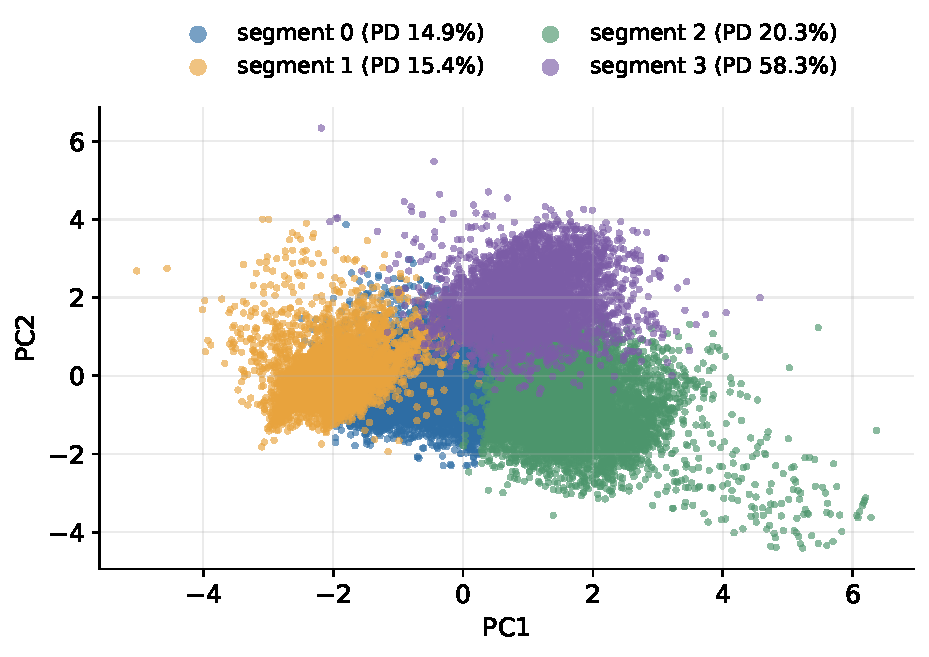
\includegraphics[width=0.56\textwidth]{lecture_4/figures/fig_pca_segments.pdf}
\caption{The $k=4$ segments in PCA coordinates, separating along the
revolving-stress axis.}
\label{fig:proj4}
\end{figure}

Projecting the segmentation onto the first two components
(Figure~\ref{fig:proj4}) shows the transactors and the distressed pulling
visibly apart along PC1 - the revolving-stress axis - with default rates
running from 15\% to 58\% across the legend: structure a strategy team
can act on.

\subsubsection{The fine print}
Four caveats, each a documented way to get PCA wrong. \emph{Scale
first}: unscaled, PC1 is simply the biggest-unit feature - the
variance-maximising direction in raw units is whatever is measured in
the largest numbers, income yet again. \emph{Variance is not
importance}: PCA never saw the target, and a direction can carry little
variance yet all the signal - the one narrow combination that predicts
default (a slight tendency to pay late while utilisation creeps up, say)
may land in PC6, and ``keep the top components'' quietly discards the
risk signal while faithfully preserving most of the variance. Check
compressed features against the supervised task before discarding
anything. \emph{Linear only}: PCA finds flat directions, and curved
structure compresses badly - a horseshoe-shaped cloud has no small set
of straight axes that represent it well.
\emph{And when components feed a supervised model, the loadings are
fitted parameters}: fit on training data only, inside the pipeline -
\texttt{make\_pipeline(StandardScaler(), PCA(5), LogisticRegression())}
- where cross-validation will refit them per fold automatically;
outside a pipeline they silently leak, Block 3's lesson in a new
costume.

For visualising curved structure, t-SNE and UMAP deserve one honest
paragraph, because their pictures are seductive. Both build a 2-D
embedding that tries to keep each point's \emph{neighbours} close, and
both sacrifice everything else to do it: the distances \emph{between}
islands mean little, the sizes and densities of the islands mean
little, and different hyperparameter settings (t-SNE's perplexity above
all) can turn one cloud into three tidy clusters or one smear - from
the same data. They are microscopes for local neighbourhood structure,
not maps of the space: use them to generate hypotheses and pictures,
never as input to downstream distances or models, and never read
cluster separation off a t-SNE plot as evidence - the algorithm
manufactures separation by design.

\subsection{Segmentation in practice}
The deliverable is the profile table: per-segment means of the clustering
features plus outcomes held \emph{out} of the clustering - and that is
where the business value appears.

\begin{center}\small
\begin{tabular}{@{}lrrrrr@{}}
\toprule
Segment & size & limit & util. & delays & default rate \\
\midrule
0 ``mainstream revolvers'' & 12{,}562 & 174k & 0.20 & 0.3 & 14.9\% \\
1 ``transactors'' & 4{,}980 & 174k & 0.03 & 0.3 & 15.4\% \\
2 ``maxed-out borrowers'' & 8{,}576 & 72k & 0.90 & 0.4 & 20.3\% \\
3 ``distressed delinquents'' & 3{,}882 & 54k & 0.60 & 4.2 & \textbf{58.3\%} \\
\bottomrule
\end{tabular}
\end{center}

Segment 3 - four months behind on average and defaulting at 58\%, over
two and a half times the portfolio's 22\% - writes its own story, and the quartet as
a whole is the classic industry segmentation (transactors, revolvers,
maxed-out, distressed) rediscovered from scratch by an unsupervised
algorithm. Read the table's logic carefully, because it is the external
leg of the validation triad in action: the clustering never saw
\texttt{default}, so the spread of default rates across segments -
14.9\% to 58.3\% - is honest evidence that the behavioural structure
carries risk information, not an echo of the target smuggled in. (Had
we clustered \emph{on} the target, the same table would prove nothing:
groups built from the answer always separate on the answer.) The table
teaches beyond risk, too: transactors default at 15.4\%, much like
mainstream revolvers - but they generate no interest income, a
profitability story rather than a risk story, and exactly the kind of
strategic fact segmentation exists to surface.

\subsubsection{Naming as a discipline}
Naming is a craft with a test: a product manager should predict the
profile from the name alone. ``Transactors'' passes - you can guess
low utilisation and full monthly repayment from the word; ``segment 1''
fails by construction; ``high-PC1-low-limit cluster'' fails the
opposite way - technically accurate, organisationally dead. Short,
concrete, slightly memorable is the target. The failure mode to fear is
dishonest naming: names imply crisp tribes where the data shows a
continuum, and our silhouette of $0.27$ says the borders are soft - so
every name travels with the soft-boundaries disclaimer earned by that
number. And write down the recipe - features, scaling, $k$, seed -
because next quarter's refresh must rebuild \emph{these} segments, not
invent new ones; a segmentation whose names change quarterly teaches
the organisation to ignore segmentations.

\subsubsection{Stability checks}
Stability is the closest thing to correctness: reseed (different random
starts - same partition? ours holds under \texttt{n\_init=10}),
resample (cluster 80\% subsamples and cross-tabulate memberships - do
customers travel together?), re-time (do next quarter's segments
reappear, or did we photograph noise?), and perturb (drop one feature
and refit - does the story survive, or did one column dictate
everything, the unscaled-income disease in disguise?). Each check
targets a different fragility: reseeding catches local optima,
resampling catches structure that lives in a handful of customers,
re-timing catches seasonal artefacts, perturbation catches
single-feature dominance. Then the strongest validator available: does
the business recognise these customers? Line managers carry an informal
segmentation in their heads; when the algorithm's segments meet theirs,
both gain credibility - and when they clash, one of the two is wrong
in an interesting way.

\begin{practice}
The sobering demonstration belongs in every practitioner's pocket: run
k-means with $k=4$ on pure uniform noise and receive four tidy,
colourful, publishable clusters (Figure~\ref{fig:noise4}). Every
clustering deliverable should survive the question \emph{``what would
this slide look like on noise?''} - the unsupervised twin of Block 1's
``torturing the data until it confesses''. A bonus recipe in the same
pocket: distance-to-nearest-centroid is a one-line anomaly score, and the
top 1\% is a serviceable first fraud shortlist with zero labels required.
\end{practice}

\begin{figure}[htbp]
\centering
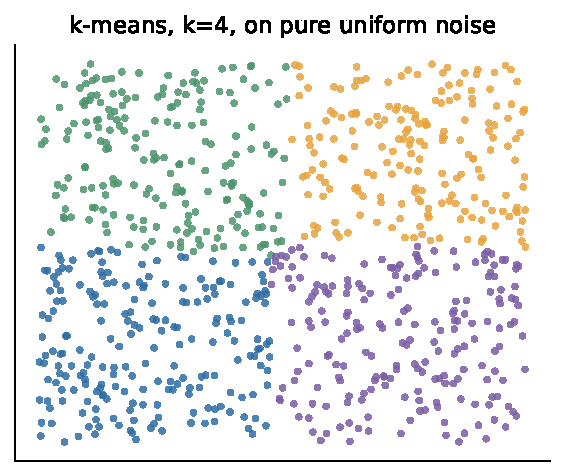
\includegraphics[width=0.4\textwidth]{lecture_4/figures/fig_noise_clusters.pdf}
\caption{Four publishable clusters on structureless noise.}
\label{fig:noise4}
\end{figure}

The noise demonstration's lesson is precise, not merely cautionary:
every internal statistic you might report - centroids, segment sizes,
a colourful 2-D scatter - exists for the noise run too. What
distinguishes the real portfolio from noise is exactly the validation
triad: silhouette (noise scores near zero at every $k$), stability
(noise clusters reshuffle under every reseed), and held-out outcomes
(noise segments show identical default rates). The demonstration is not
an argument against clustering; it is the argument for validating it.
The anomaly recipe, meanwhile, upgrades Block 1's lesson about
outliers: a customer far from every centroid matches no known
behavioural pattern - a data error, a fraud case, or a customer type
you have not met yet, and worth a human look in all three cases;
DBSCAN's noise bucket delivers the same shortlist for free.

Where segments are allowed to work: strategy and product design; drift
monitoring (segment sizes over quarters as a leading indicator, tying
into Block 3's monitoring - a growing ``maxed-out'' segment tells you
something no single account shows); communication (tone and channel per
segment); and as features in supervised models - with the clustering
fitted on training data only, the golden rule following us everywhere. Where they are not:
as the individual credit decision - pricing a person by their segment
invites regulatory trouble and unfairness (Block 6 returns to fairness
properly). The common sins, for the record: clustering on the target or
its twins (manufactured foresight - Block 3's leakage in a new
costume); unscaled features (one column secretly dictates the whole
segmentation); more segments than anyone can name (fourteen segments is
a lookup table, not insight); hard-boundary storytelling on a
continuum; quarterly refits that re-derive ``new'' customer types from
seed noise; and never asking the noise question.

\subsection{Lab and hand-in}
The lab notebook \texttt{04\_clustering\_pca} walks the arc: break
clustering with unscaled features, then scale; choose $k$ with elbow and
silhouette and read the weak signals honestly; profile and name the
$k=4$ segments (with the honesty clause); a Ward dendrogram on a sample;
DBSCAN versus k-means on crescents; PCA's scree, loadings and 2-D
projection; and the noise demonstration. Exercises cover reseeding and
resampling stability, feature-drop perturbation, the anomaly shortlist,
Gaussian-mixture soft memberships, and PCA-as-features inside the Block 3
tournament pipeline - expect no miracle on our compact feature set;
the point is the pattern, which pays off on wide, correlated data. ``Done''
means the segment names pass the product-manager test and the honesty
paragraph would survive a sceptical reviewer. Project checkpoint: both
model families should exist this week, however rough, so the final
fortnight belongs to evaluation and the slides; and any project
segmentation must arrive with the honesty kit - silhouette or
stability evidence, the soft-boundaries sentence, and named profiles; a
pretty scatter plot is not a deliverable.

% =====================================================================
\section{Block 5 - Pattern discovery \& text mining}

Two new datasets join the course, both about the same 4{,}000 customers:
which of ten \emph{products} each holds
(\texttt{finance\_data.load\_baskets()}) and 1{,}200 labelled customer
\emph{complaints} (\texttt{load\_complaints()}). They carry the block's two
crafts - mining co-occurrence patterns, and turning text into features
- plus a supervised comeback: the multiclass classification promised on
Block 1's map. The two crafts look unrelated but share a skeleton: both
force a messy object (a basket, a sentence) into one wide, sparse
matrix, both then let the rest of the course loose on it, and both need
the same honesty checks at the end - wide sparse matrices are exactly
where spurious structure loves to hide.

\subsection{Baskets and association rules}
The abstraction is one binary table, transactions $\times$ items - the
literal shopping basket in retail, co-prescriptions in medicine, pages per
session on the web, and in fraud work the shared devices and phone numbers
that expose application rings. Ours is product cross-holding
(Figure~\ref{fig:basket5}): sparse, binary, one row per customer. The
business question: which products travel together - and which pairing is
genuine affinity rather than a coincidence of popularity? Building the
matrix is a \texttt{TransactionEncoder} or one \texttt{pd.crosstab} away
- after answering Block 1's question (what is a row? one visit or one
customer-lifetime?) whose answer the mined rules inherit. Add timestamps
and the question upgrades to sequences - \emph{what comes next} - the
customer-lifecycle version we only mention.

The reach of the abstraction is worth dwelling on, because it decides
whether you will recognise a basket problem when it does not arrive in a
shopping trolley. Whenever you can name a \emph{transaction} (a customer,
a hospital admission, a browsing session, a loan application) and an
\emph{item} vocabulary (products, drugs, pages, phone numbers), you can
build the table and everything in this chapter applies. In medicine the
rules are co-morbidities and drug-interaction candidates; on the web they
are ``customers who viewed this also viewed''; in fraud the direction
reverses - there the \emph{surprising} co-occurrence (five applications
sharing one device) is the alarm, not the campaign. And note what the
row-definition question does to the output: if a retail row is one visit,
the rules describe what lands in one trolley together (beer and crisps);
if a row is one customer-year, the rules describe lifestyles (nappies and
baby food). Neither is wrong - but a campaign built on the wrong grain
answers a question nobody asked.

\begin{figure}[htbp]
\centering
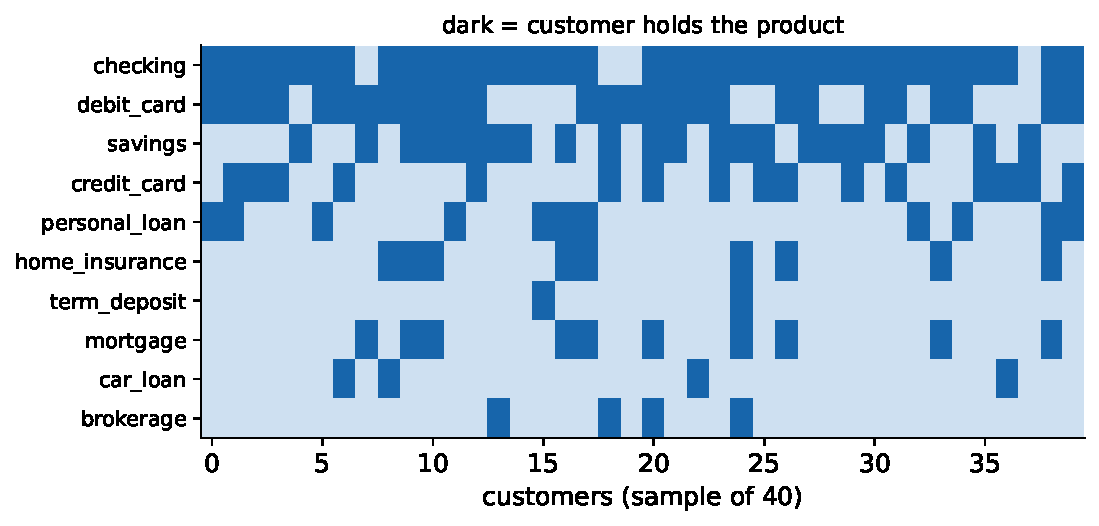
\includegraphics[width=0.72\textwidth]{lecture_5/figures/fig_basket_sample.pdf}
\caption{The basket matrix: binary, sparse, mineable.}
\label{fig:basket5}
\end{figure}

\subsubsection{Support, confidence, lift - the three numbers}
An \emph{itemset} is any set of products; its \emph{support} is the share
of customers holding all of it (single-item supports are just penetration
rates, Figure~\ref{fig:pen5}). A \emph{rule} $A \Rightarrow B$ reads
``holders of $A$ tend to hold $B$'' - the arrow is our reading
direction, not causality. Three numbers rank rules:
\[
  \text{support} = \frac{n_{A\cup B}}{n}, \qquad
  \text{confidence} = \frac{n_{A\cup B}}{n_A} = P(B \mid A), \qquad
  \text{lift} = \frac{P(B \mid A)}{P(B)} .
\]
Support is materiality, confidence is the reliability of the promise, lift
is surprise - how much more often than chance, with 1 meaning
independence. The probability identities deserve one slow reading.
Support is the joint probability $P(A \cap B)$ estimated by a count;
confidence is the conditional probability $P(B \mid A)$, which by
definition equals $P(A \cap B)/P(A)$ - support of the pair over support
of the antecedent; and lift is
\[
  \text{lift}(A \Rightarrow B)
  = \frac{P(B \mid A)}{P(B)}
  = \frac{P(A \cap B)}{P(A)\,P(B)},
\]
the observed joint probability divided by what independence would
predict. The second form makes two facts obvious: lift is symmetric
(lift of $A \Rightarrow B$ equals lift of $B \Rightarrow A$, which is why
mirror rules always share it), and lift $=1$ is exactly the definition of
statistical independence.

A toy contingency table makes the three numbers concrete. Take 100
customers; 40 hold product $A$, 30 hold product $B$, 20 hold both:

\begin{center}\small
\begin{tabular}{@{}lccc@{}}
\toprule
 & holds $B$ & no $B$ & total \\
\midrule
holds $A$ & 20 & 20 & 40 \\
no $A$    & 10 & 50 & 60 \\
\midrule
total     & 30 & 70 & 100 \\
\bottomrule
\end{tabular}
\end{center}

Then $\text{supp}(A \Rightarrow B) = 20/100 = 0.20$,
$\text{conf} = 20/40 = 0.50$, and
$\text{lift} = 0.50 / 0.30 \approx 1.67$: $A$-holders take $B$ at
1.67 times the population rate - a real attraction, though a modest
promise (only half convert). All three numbers come from the same four
cells; when a rule confuses you, reconstruct its table.

\begin{figure}[htbp]
\centering
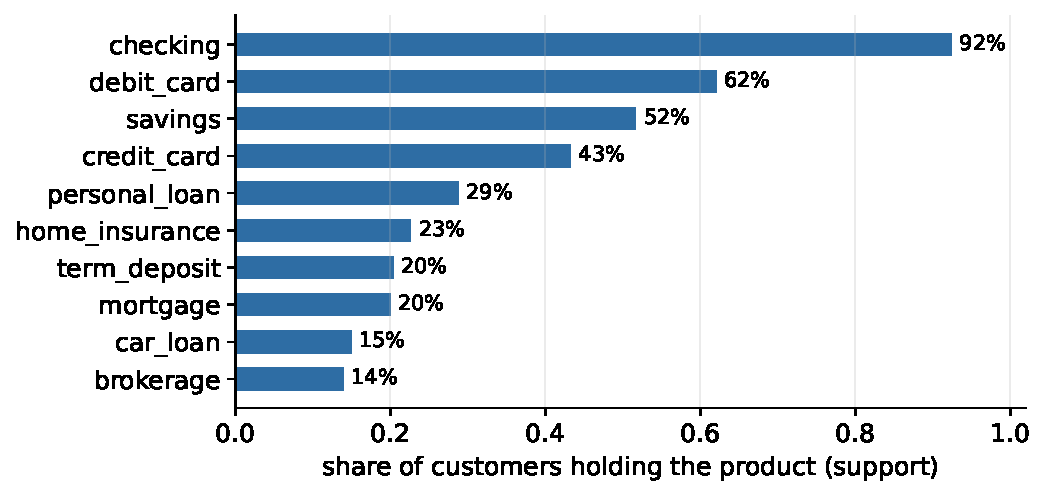
\includegraphics[width=0.62\textwidth]{lecture_5/figures/fig_penetration.pdf}
\caption{Single-item supports: product penetration.}
\label{fig:pen5}
\end{figure}

Worked on our data: 800 mortgage holders, 906 insurance
holders, 678 with both, so support $678/4000 = 0.17$, confidence
$678/800 = 0.85$, lift $0.85/0.227 \approx 3.7$ - and the actionable
list is the rule's \emph{complement}, the 15\% of mortgage holders without
the bundle. Read the rule aloud, all three numbers in one sentence:
\emph{17\% of customers hold both; 85\% of mortgage holders have the
insurance - 3.7 times more often than a random customer.} The deck's
sixty-second exercise runs the same arithmetic on
brokerage $\Rightarrow$ deposit (558 brokerage holders, 815 deposit
holders, 359 with both: support $\approx 0.09$, confidence
$\approx 0.64$, lift $\approx 3.2$) - a weaker promise, the same
verdict: genuine affinity, the affluent-saver pattern Block 4's
segmentation already sketched.

\subsubsection{The confidence trap, in full}
Here is the arithmetic that makes the trap inescapable rather than
merely plausible. Confidence is $P(B \mid A)$ - and if $B$ is held by
nearly everyone, then $P(B \mid A)$ is high for \emph{any} $A$
whatsoever, informative or not. Condition on holding a savings account,
condition on owning a red umbrella: either way the share with a checking
account hovers near the base rate, because the base rate is where
conditional probabilities live when the conditioning event carries no
information. Formally, $A$ independent of $B$ gives
$P(B \mid A) = P(B)$ exactly - so a 92\%-penetration consequent
guarantees roughly 92\% confidence \emph{for free}. Confidence answers
``how reliable is the promise?''; only lift answers ``is there a
relationship at all, beyond chance?'' - it is the ratio that divides
the promise by what no-information would already deliver.

\begin{practice}
The confidence trap, from our own output: \texttt{savings} $\Rightarrow$
\texttt{checking} boasts 92.7\% confidence - against a 92.4\% base rate.
Lift 1.003: pure base-rate flattery, Block 2's accuracy trap wearing a
basket. The two traps are literally the same fraction: a majority-class
classifier is ``93\% accurate'' and an everybody-has-it consequent is
``93\% confident'', and in both cases the impressive number was
inherited, not earned. Rule hygiene in one line: filter by support, rank
by lift, read confidence for the campaign promise. And deduplicate: one
mortgage--insurance affinity surfaces as a dozen rules - both
directions, re-decorated with irrelevant extras
(Figure~\ref{fig:toprules5}) - one insight in ten costumes.
\end{practice}

\begin{figure}[htbp]
\centering
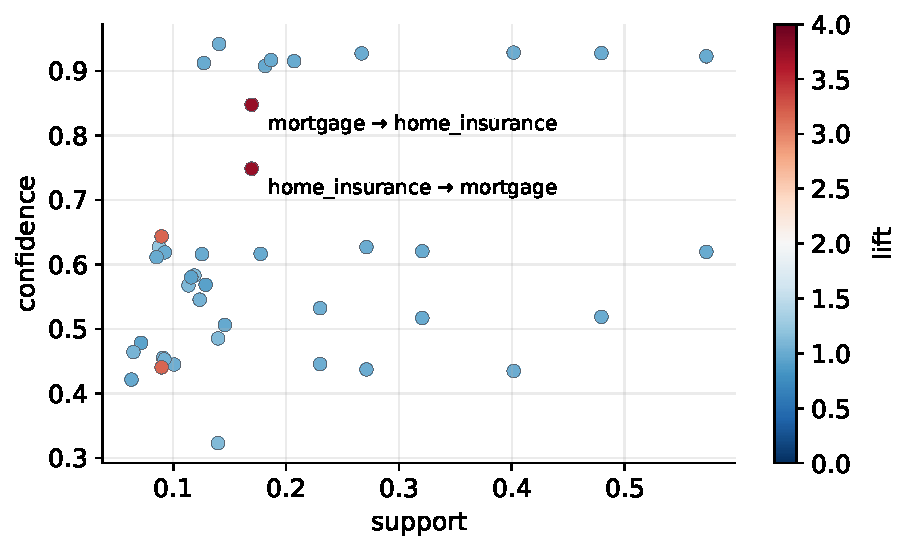
\includegraphics[width=0.68\textwidth]{lecture_5/figures/fig_rules_scatter.pdf}
\caption{The rule landscape: most rules crowd lift $\approx 1$.}
\label{fig:scatter5}
\end{figure}

The rule landscape (Figure~\ref{fig:scatter5}) is worth memorising: a
dense crowd at lift $\approx 1$ - popular items co-occurring by
arithmetic, not affinity - and a handful of outliers worth a meeting.
The discipline (filter, rank, deduplicate) exists precisely to fish the
outliers out of that crowd.

\begin{figure}[htbp]
\centering
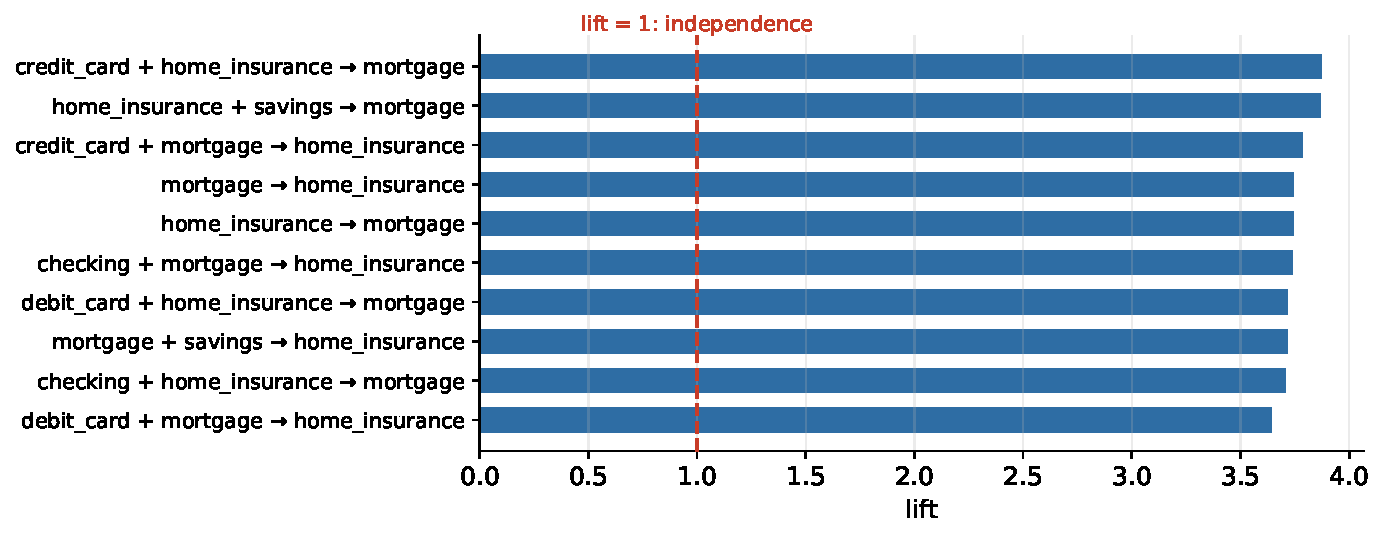
\includegraphics[width=0.74\textwidth]{lecture_5/figures/fig_top_rules.pdf}
\caption{Top rules by lift - note the redundancy.}
\label{fig:toprules5}
\end{figure}

\subsubsection{Redundancy, and the numbers beyond the big three}
Acting on rules deserves its own honesty. The 15\%-without-insurance call
list may differ exactly in whatever made them decline the bundle; the
honest upgrade is an experiment - hold out a control group, measure
uplift, not response. And expect feedback: acting on a pattern changes it,
so rules are re-mined on fresh data and rule lists carry dates.
Association rules \emph{nominate} actions; experiments \emph{validate}
them. Beyond the big three, leverage
($P(A \cap B) - P(A)P(B)$) resists tiny-support flattery; conviction,
$(1 - \text{supp}(B)) / (1 - \text{conf}(A \Rightarrow B))$, rephrases
confidence against independence (1 means independent, $\infty$ means
never wrong); and closed/maximal itemsets compress the inventory.

Conviction rewards one more sentence, because its formula looks opaque
until you read it as a ratio of error rates. The numerator
$1 - \text{supp}(B)$ is how often the rule \emph{would} be wrong if $A$
told us nothing (a random customer lacks $B$ that often); the denominator
$1 - \text{conf}$ is how often the rule \emph{is} wrong. Conviction
therefore says ``the rule fails this many times less often than
independence would''. On the toy table above:
$(1 - 0.30)/(1 - 0.50) = 1.4$ - the rule is wrong 1.4 times less often
than chance. Unlike lift it is direction-sensitive, which occasionally
breaks the tie between a rule and its mirror.

Redundancy is not a cosmetic nuisance; it is a reporting hazard. Because
lift is symmetric, every affinity ships as two rules; because adding a
near-universal item to either side barely moves the numbers, each of the
two spawns decorated variants (\texttt{+ checking},
\texttt{+ debit\_card}). A ten-slide ``insights deck'' can easily contain
one insight. The professional discipline: collapse mirrors, drop rules
whose antecedent is a superset of a simpler rule with the same consequent
and no better lift, and report each surviving affinity once - with all
three numbers and one honest sentence.

\subsection{Mining at scale}
Brute force dies immediately: $2^p - 1$ itemsets to count. At our
$p = 10$ that is a harmless 1{,}023; at a supermarket's
$p = 30{,}000$ it is astronomy, and yet stores mine baskets every night.
The rescue is the \textbf{Apriori principle} (downward closure): every
subset of a frequent itemset is frequent - equivalently, an infrequent
itemset's supersets are infrequent and need never be counted.

\subsubsection{Downward closure, proved in three sentences}
Every customer who holds all items of a set $S$ also holds all items of
any subset $T \subseteq S$ - holding more can only shrink the set of
qualifying customers, never grow it. Hence
$\text{supp}(T) \geq \text{supp}(S)$ whenever $T \subseteq S$: support
is monotonically non-increasing as itemsets grow. So if $T$ already
fails the support threshold, every superset $S \supseteq T$ fails it
too - and an algorithm may skip all of them without counting a single
one. That is the entire mathematical content of Apriori; everything else
is bookkeeping.

\subsubsection{The level-wise search and its economics}
Apriori (1994) applies the principle level-wise: count the support of all
1-itemsets and prune the infrequent ones; build candidate 2-itemsets
\emph{only from surviving} 1-itemsets and count those; build candidate
3-itemsets only from pairs of surviving 2-itemsets, checking that every
2-subset survived; repeat until a level produces no candidates. The deck's
five-customer toy shows the mechanism end to end: with min-support at
2-of-5, \{leasing\} dies at level one, so \{leasing, \emph{anything}\} is
never even generated; \{loan, deposit\} dies at level two, so the only
conceivable 3-itemset \{card, loan, deposit\} is pruned before counting
because one of its subsets already failed. The economics: the exponential
candidate space is tamed because each pruned itemset takes its entire
superset cone with it, and in sparse data almost everything is pruned
early. The cost that remains is I/O - every level re-scans the data -
which Apriori accepts in exchange for simplicity and easy
parallelisation.

The throttle on the whole machine is \texttt{min\_support}, and it is a
business number, not a tuning knob: ``rules touching $<$3\% of customers
cannot fund a campaign'' is the right sort of justification. Its
consequences run in both directions. Set it too low and the candidate
levels stop pruning: the frequent-itemset inventory explodes, the rule
list balloons into thousands of fragile patterns each supported by a
handful of customers, and multiple testing - which is built into the
method, since every itemset is a hypothesis - guarantees that many are
noise. Set it too high and only the obvious survives:
\texttt{checking} co-occurs with everything, and the list becomes a
penetration report. And since retail's interesting items are
individually rare, long-tail catalogues get mined at category level
(``any insurance product'') where supports are honest.

\subsubsection{FP-Growth, honestly}
FP-Growth (2000) reaches the identical output by a different route: it
compresses the baskets into a prefix tree (the FP-tree) in which
customers sharing frequent prefixes share branches, then mines the tree
recursively, extracting each item's ``conditional'' subtree and recursing
on it - no candidate generation at all, and only two scans of the data.
That is the whole honest story: same definitions, same frequent itemsets,
same rules; the win is engineering (memory locality, no repeated I/O),
which is why it is the usual industrial choice, and why at our $p = 10$
you cannot measure the difference. \texttt{mlxtend} ships both. Whatever
the miner, output discipline is fixed: filter support, rank lift,
deduplicate, then read.

\subsection{Text becomes numbers}
Banks are full of unmined text - complaints, chats, advisor notes. Our
corpus: 1{,}200 complaints, five categories (card fraud, mortgage, fees,
app \& service, collections), and the target task of routing each to the
right team. Models eat numbers, so the craft is the bridge: strings to a
feature matrix, in four deliberate steps. \emph{Normalise} (lowercase,
punctuation - decisions, not defaults); \emph{tokenise};
\emph{count} - the bag of words, one column per token, word order
discarded on purpose (``the bank closed my account'' equals ``my account
closed the bank''); \emph{weigh} - TF-IDF. Each step throws information
away on purpose; the art is knowing what you can afford to lose.

\subsubsection{Tokenisation decisions are modelling decisions}
The normalisation submenu is feature engineering by another name, and
every default hides a claim about your problem. Lowercasing asserts that
\emph{Bank} and \emph{bank} mean the same thing - usually true, false
for tickers and product names. Stripping punctuation asserts that
``24/7'' and ``PLN'' and exclamation marks carry nothing - yet in
complaint text, punctuation density is a decent anger proxy. Stopword
lists shrink the matrix but a default list happily deletes \emph{not}
(``not refunded''!) - a single deleted token that reverses the meaning
of a sentence; audit any list before trusting it. Stemming chops endings
fast and crudely (\emph{charged, charges, charging} collapse to one
column - efficient, occasionally comic); lemmatisation reduces to
dictionary base forms and earns its keep in morphology-rich languages -
Polish's \emph{opłata, opłaty, opłatom, opłatach} are one lemma and four
bag-of-words strangers, with character n-grams as the robust fallback and
multilingual embeddings largely dissolving the problem. Every one of
these choices merges or splits columns of the future matrix; the
discipline is the same as for any engineered feature - document the
recipe, and keep it identical between training and production, because a
router trained on lemmatised text and fed raw inflections is comparing
strangers.

\begin{figure}[htbp]
\centering
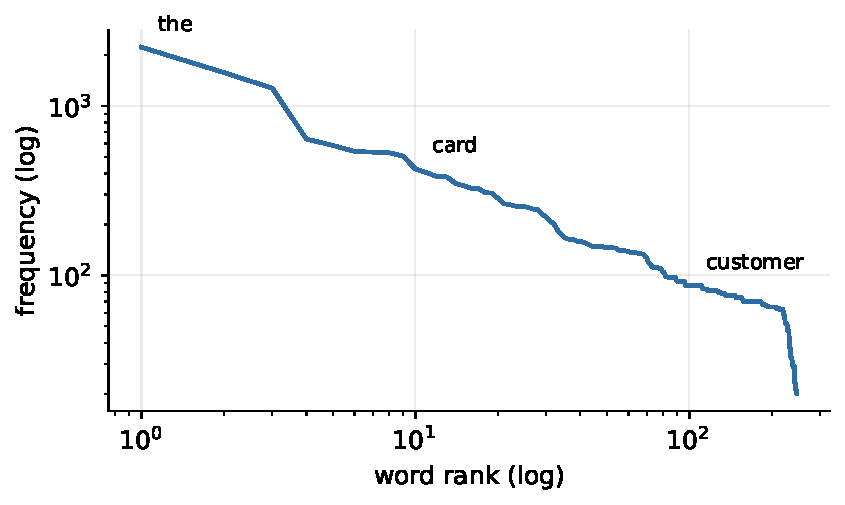
\includegraphics[width=0.56\textwidth]{lecture_5/figures/fig_zipf.pdf}
\caption{Zipf's law in the complaint corpus.}
\label{fig:zipf5}
\end{figure}

\subsubsection{Zipf's law and what it implies}
Every corpus obeys Zipf's law (Figure~\ref{fig:zipf5}): a few words
everywhere, most words rare, a near-line on log-log axes -
frequency falling roughly as one over rank. Both ends are
trouble - the head carries no distinction, the tail no statistics -
and \texttt{max\_df}/\texttt{min\_df} are the vectoriser's leash. The
law has a consequence worth stating explicitly, because it drives half
the engineering in this section: as the corpus grows, the
\emph{vocabulary} keeps growing (new rare words keep arriving,
essentially forever) while the \emph{information} does not grow with it
- each new column is rarer, appears in fewer documents, and supports
weaker statistics than the last. Feature matrices built from text
therefore widen without bound unless pruned, and pruning the tail with
\texttt{min\_df} is nearly free: a token seen in one document cannot
generalise to a second one anyway.

\subsubsection{TF-IDF, with the arithmetic on the table}
TF-IDF then weighs each count by rarity,
\[
  w_{d,t} = \text{tf}_{d,t} \times
  \Bigl(\ln\tfrac{1 + n_{\text{docs}}}{1 + n_{\text{docs with } t}} + 1\Bigr),
\]
so \texttt{account} costs almost nothing while \texttt{skimmed} and
\texttt{casino} scream card fraud (Figure~\ref{fig:idf5}); length
normalisation keeps rambling complaints from outweighing terse ones. A
tiny worked example fixes the mechanics. Take a four-document corpus and
a document in which some term appears 3 times. If the term occurs in all
four documents, its idf is $\ln\frac{1+4}{1+4} + 1 = \ln 1 + 1 = 1$:
weight $3 \times 1 = 3$, the raw count, no boost - ubiquity buys
nothing. If instead it occurs in only two documents, idf is
$\ln\frac{5}{3} + 1 \approx 0.51 + 1 = 1.51$: weight
$3 \times 1.51 \approx 4.5$. Same count, half the corpus coverage, fifty
percent more weight - and the rarer the term, the steeper the boost.
Note that idf is a \emph{corpus} statistic: it is estimated from the
training documents and then applied, frozen, to every future document -
which is why it is a fitted parameter and why it leaks if computed on
the full dataset before the split.

\begin{figure}[htbp]
\centering
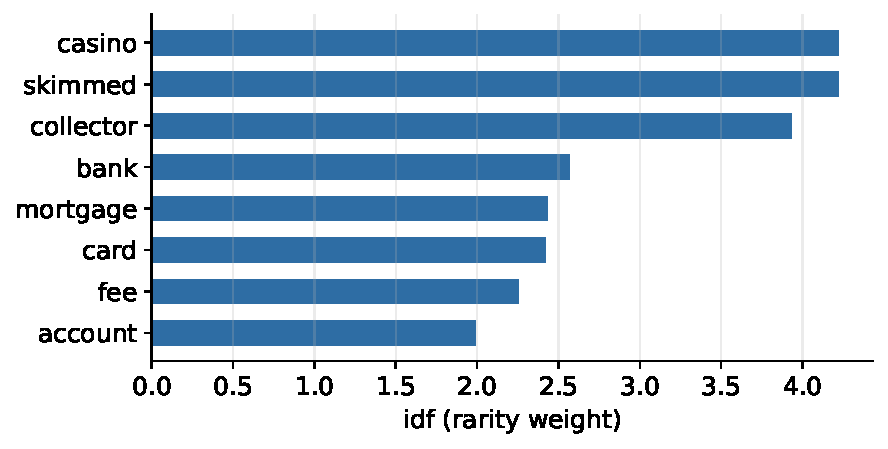
\includegraphics[width=0.46\textwidth]{lecture_5/figures/fig_idf_words.pdf}
\caption{idf in our corpus: rarity as a weight.}
\label{fig:idf5}
\end{figure}

\subsubsection{N-grams, sparsity, and cosine}
N-grams buy back fragments of word order - \emph{collection calls},
\emph{unauthorized transactions} - worth three accuracy points on our
corpus at the price of a vocabulary explosion ($247 \to 865$ features;
real corpora shed thousands of one-off tokens to \texttt{min\_df} with no
loss). The trade is always the same shape: longer n-grams capture more
context and appear less often, so each added order buys specificity and
pays in Zipf-tail sparsity - word bigrams are usually worth it,
trigrams rarely, beyond that almost never for classification. Character
n-grams run the same trade at the sub-word level: a 3--5 character window
slides over the string, so \emph{opłata} and \emph{opłatach} share most
of their features automatically, typos cost one n-gram instead of a
whole word, and morphology-rich languages get robustness that word
tokens cannot offer - the standard fallback when no good lemmatiser
exists.

The resulting matrix is $\sim$90--97\% zeros - a complaint uses a few
dozen distinct words of a vocabulary of hundreds - and sparsity is not
a defect but the resource that makes text mining affordable. Sparse
storage keeps only the non-zero entries, megabytes instead of gigabytes;
sparse-aware linear algebra multiplies only what is stored, so training
cost scales with the number of \emph{words in the corpus}, not with the
matrix's nominal area. That is why wide text models stay fast - and one
more reason wide-and-sparse is linear-model country. The practical
corollary from the lab: never densify a sparse matrix ``just to look'';
that single \texttt{.toarray()} is how notebooks die.

For distances, cosine similarity compares direction rather than length,
\[
  \cos(\theta) = \frac{x \cdot y}{\lVert x \rVert \, \lVert y \rVert},
\]
- Block 4's ``distance is a modelling choice'', text edition. The
reason length-normalisation matters is mechanical: a long and a short
complaint about the same fraud contain the same word \emph{mix} but very
different word \emph{amounts}, so Euclidean distance places them far
apart on length alone. Dividing by the norms erases document length and
compares only proportions - two documents about skimmed cards are close
whether one is a paragraph and the other a page. And once text is
columns, the whole course applies: EDA on top words, clustering
complaints, truncated SVD as latent semantic analysis, and
classification - next.

\begin{figure}[htbp]
\centering
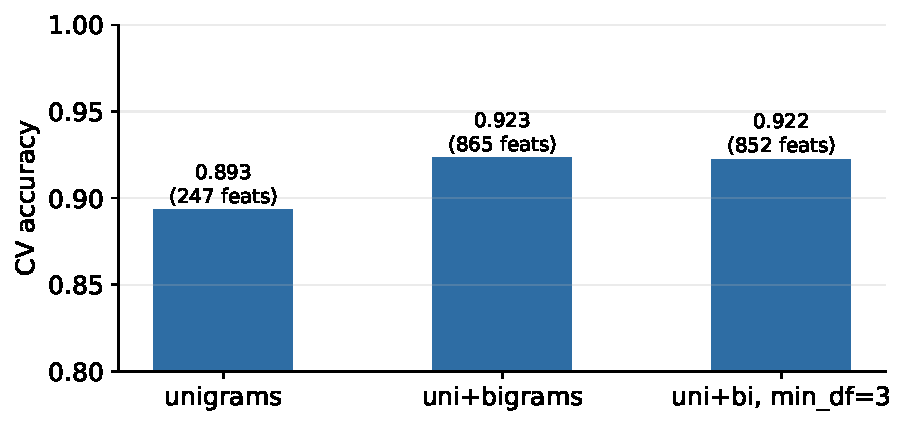
\includegraphics[width=0.6\textwidth]{lecture_5/figures/fig_ngram_effect.pdf}
\caption{N-grams buy accuracy and cost dimensions.}
\label{fig:ngram5}
\end{figure}

\subsection{Classifying complaints}
The router is two familiar pieces - a \texttt{TfidfVectorizer} welded to
\texttt{LogisticRegression} in a pipeline - with the golden rule in its
text edition: vocabulary and idf are fitted parameters, so the vectoriser
fits on training data only. Test accuracy:
\textbf{90.3\%} on five balanced classes against a 20\% chance floor
(Figure~\ref{fig:conf5}), with errors concentrated exactly where
complaints ramble across topics - the cases a human router also flags.
Balanced classes make accuracy honest here; real complaint streams are
imbalanced, and then per-class recall and macro-F1 (each class weighted
equally) take over, with the worst class - not the average - being
the number that pages you.

\subsubsection{Why linear models rule sparse text}
It is worth pausing on why so unfashionable a model wins here, because
the reason generalises. A TF-IDF matrix has thousands of columns, each
individually weak (\emph{casino} appears in a handful of documents) but
collectively decisive, and each acting near-additively: more fraud words,
more fraud evidence. That is precisely the regime a regularised linear
model is built for - it can carry a coefficient for every column,
regularisation keeps the thousands of weak coefficients from overfitting,
and sparse arithmetic makes the whole thing fast. Trees, by contrast,
must pick one feature per split; with signal smeared thinly across
thousands of near-binary columns, axis-by-axis splitting wastes most of
the evidence, which is why GBDT rarely beats logistic regression on raw
sparse text. Add interpretability - a coefficient per word per class is
an audit trail - and linear-on-TF-IDF remains the default that
alternatives must beat.

\subsubsection{Naive Bayes in one derivation sketch}
Naive Bayes remains the classical fast baseline
(\texttt{MultinomialNB}; the baseline discipline says try it), and its
logic fits in four lines. Bayes' rule gives
$P(c \mid d) \propto P(c)\, P(d \mid c)$; the ``naive'' step assumes
words are independent given the class, so
$P(d \mid c) \approx \prod_t P(t \mid c)^{\text{tf}_{d,t}}$, with each
$P(t \mid c)$ estimated by a smoothed count: how often word $t$ appears
in class-$c$ training documents. Take logarithms and the classifier
scores each class by
$\log P(c) + \sum_t \text{tf}_{d,t} \log P(t \mid c)$ - a linear
function of the counts, which is why NB and logistic regression are
siblings: same functional form, differently estimated weights. The
independence assumption is plainly false (\emph{collection} and
\emph{calls} travel together), so the estimated probabilities are badly
calibrated - but classification needs only the \emph{ranking} of class
scores, and correlated words mostly inflate all class scores together
without flipping the winner. Wrong model, right argmax - which is why
NB classifies far better than it estimates, and why it filtered the
world's spam for decades.

\begin{figure}[htbp]
\centering
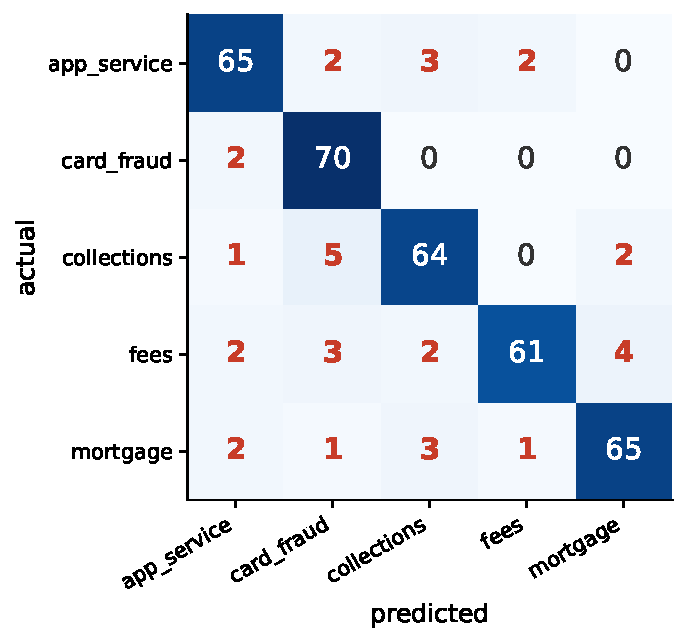
\includegraphics[width=0.44\textwidth]{lecture_5/figures/fig_confusion_text.pdf}
\caption{The router's confusion matrix (test set).}
\label{fig:conf5}
\end{figure}

\subsubsection{Reading the router, then operating it}
Interpretability carries over intact: top coefficients per class
(Figure~\ref{fig:words5}) are a sanity check you can read - fraud
listens for \emph{card, payments, online}; collections for
\emph{collector, calls}; mortgage for \emph{agreement, contradicts} -
and an off-topic top word is the leakage smell, text edition (imagine
\emph{refunded} predicting fraud, written after resolution). Read the
confusion matrix (Figure~\ref{fig:conf5}) the same way you read Block
3's: the diagonal is comfort, the off-diagonal cells are the product.
Each off-diagonal cell is a specific routing failure with a specific
cost - fees complaints landing in the mortgage queue waste a
specialist's morning; fraud complaints landing anywhere else delay a
card block - and ``done'' in the lab explicitly requires an explanation
per cell, because a cell you cannot explain is a cell you cannot fix.

\begin{figure}[htbp]
\centering
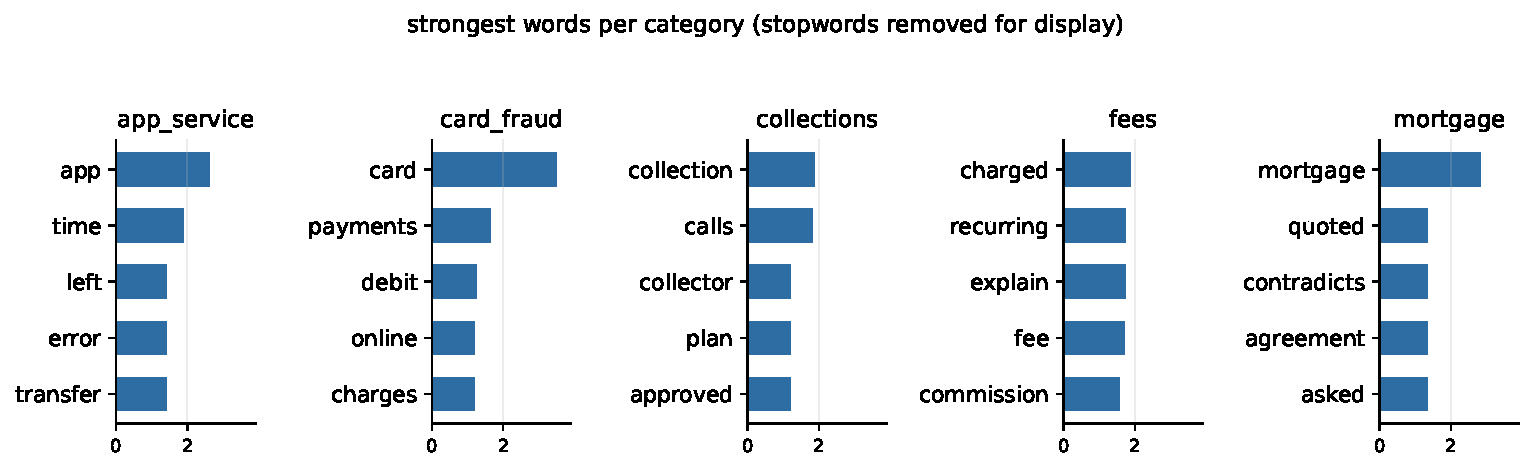
\includegraphics[width=0.92\textwidth]{lecture_5/figures/fig_class_words.pdf}
\caption{What the model reads: top words per category.}
\label{fig:words5}
\end{figure}

Operations adds Block 3's threshold logic in multiclass form: route
automatically only above a confidence bar. On our test set, a 0.6 bar
auto-routes 81\% of complaints at 98.3\% accuracy and queues the hard
19\% for humans - the bar chosen with the operations team, not by the
data scientist alone. The sweep around that point shows the trade
explicitly: no bar means 100\% automation at 90.3\% accuracy; a 0.5 bar
auto-routes 91\% at 93.6\%; 0.6 gives 81\% at 98.3\%; 0.7 gives 79\% at
100\% on this test set. The economics behind the choice are Block 3's
expected-cost logic verbatim: every point of the bar trades automation
volume (human minutes saved) against auto-routing errors (misfiled
complaints, each with a cleanup and reputation cost), and the right bar
depends on numbers only the operations team has. The human queue is not
an admission of failure - it is the design: human attention
concentrates exactly where the model itself signals difficulty.

Embeddings and LLMs are the modern bridge - dense vectors where ``the
app crashes'' and ``application keeps freezing'' finally meet - feeding
the same classical models: Block 2's feature-factory promise delivered,
with TF-IDF still winning when data is small, latency and cost matter,
and the auditor asks why. The shop rule is Block 3's discipline
verbatim: start with TF-IDF plus logistic, and let embeddings
\emph{earn} their complexity against that baseline.

\subsection{Pitfalls of both crafts}

\subsubsection{The shuffled-basket null test}
The sobering demonstration, basket edition: shuffle every product column
independently (killing all co-occurrence, keeping all penetrations) and
re-mine with identical settings - 312 ``rules'' still pass the filters,
against 545 on the real data. The rule \emph{count} is nearly
meaningless; what noise cannot fake is lift: 1.14 versus 4.28. Recognise
the move: this is Block 4's noise question - \emph{what would this
deliverable look like on data with no structure?} - answered with a
number instead of a shrug, the unsupervised cousin of a permutation
test. Shuffling each column independently preserves every marginal
(penetration rates are untouched) while destroying every joint pattern,
so anything the miner still ``finds'' is pure arithmetic of popular
items co-occurring by chance under the filters. The 312 phantom rules
calibrate your scepticism: a rule from real data impresses only to the
extent that its lift clears what the shuffled world produces. The test
costs five lines of code and should accompany any mined-rules
deliverable, for the same reason a shuffled-label baseline accompanies a
classifier.

\subsubsection{Text hygiene and the joint sin list}
Text hygiene mirrors it: the vectoriser inside the pipeline (vocabulary
leaks too - a vocabulary or idf computed on the full corpus has seen
the test documents, and rare-word idf is the sharpest leak); vocabulary
drift over time (out-of-time testing applies to text, and deserves
monitoring in production: new products, new slang and new fraud patterns
arrive as words the fitted vocabulary has never seen, the router's
failure is \emph{silent} - out-of-vocabulary tokens are simply dropped,
and the complaint is confidently misfiled into the nearest old category
- so the minimal monitoring watches the prediction-confidence
distribution for a growing low-confidence mass, per-class routing rates
against baseline, and a small ongoing human-labelled sample, with
retraining triggered by drift, not by the calendar); PII living inside
free text (anonymise before mining - GDPR is not a footnote); and
language reality beyond our conveniently English corpus. The joint sin
list: confidence without lift; one insight in ten costumes; reading
rules causally; stopword cargo-culting; evaluating text models on
near-duplicate documents across the split - templated complaints
landing on both sides of it are the duplicate leak, text edition; and
shipping a router with no human queue - 90\% right means one complaint
in ten lands on the wrong desk, silently.

\subsection{Lab and hand-in}
The lab notebook \texttt{05\_pattern\_mining\_text} mines the baskets
(penetration, Apriori, rules, the confidence trap on live output), runs
the shuffled-basket sobering check, builds the text bridge (Zipf, TF-IDF,
idf spot-checks), trains and audits the router (classification report,
confusion matrix, misrouted examples - which visibly ramble), operates
it with a confidence bar, and reads the per-class top words. Exercises add
n-grams, the Naive Bayes bake-off, a \texttt{min\_support} sweep ending in
a reporting decision, complaint clustering (Block 4 meets Block 5),
character n-grams for robustness, and a drift stress-test. ``Done'' means
three rules that survive the lift-versus-confidence interrogation and a
confusion matrix whose every off-diagonal cell has an explanation. Project
checkpoint: two weeks to the presentation - interpretation, a written
recommendation, and the presentation skeleton belong to this week, and the
code-plus-slides upload lands before Block 7. If your project touches
baskets or text, the honesty kit extends to it directly: lift over
confidence, deduplicated rules, the vectoriser inside the pipeline, and
one out-of-vocabulary sentence in the limitations.

% =====================================================================
\section{Block 6 - Neural networks \& responsible ML}

The last teaching block does two jobs. It completes the model-family tour
with the one family everyone has heard of - honestly, foundations first,
entered into the same tournament as everyone else. And it assembles the
course's scattered responsibility threads - selection bias, truthful
reasons, segments that must not decide, PII - into one section with our
own model's numbers in it.

\subsection{From the neuron to the MLP}

\subsubsection{One neuron is Block 2, wearing a new hat}
A neuron is a weighted sum squashed through a nonlinearity,
$\sigma(w_0 + w_1 x_1 + \dots)$ - which the attentive reader of Block 2
recognises immediately: one neuron with a sigmoid \emph{is} logistic
regression. Write both out and compare symbol by symbol. Logistic
regression computes $p = \sigma(w_0 + w_1 x_1 + \dots + w_d x_d)$ with
$\sigma(z) = 1/(1+e^{-z})$; a single sigmoid neuron computes exactly the
same expression. Same weights, same bias (the intercept under a new
name), same squashing function, and - as we will see shortly - the same
loss. The correspondence is not an analogy; it is an identity, and it
means everything you fear about neural networks already has a Block 2
anchor: weights as slopes, sigmoid as probability, log-loss as the
objective.
(The perceptron dates to 1958 - older than CRISP-DM and credit scoring;
two AI winters later, data and GPUs made the mathematics bloom largely
unchanged.)

What changes everything is not the neuron but the \emph{stacking}. The
multilayer perceptron (MLP) arranges neurons in layers: each hidden unit
computes its own logistic-like score of the layer below, and the next
layer combines \emph{those} scores rather than the raw features. Where
logistic regression sees `utilisation' and `delays' as given columns, a
hidden unit can learn to fire on `high utilisation \emph{and} recent
delays together' - a derived feature nobody typed in. The network
thereby \textbf{engineers its own features} - Block 1's craft, automated
- which is the entire selling point. Depth composes: layer two builds
combinations of layer one's combinations, so the representational
vocabulary grows multiplicatively with each layer while the parameter
count grows only additively.

\subsubsection{The XOR lesson: why linear models need hand-fed
interactions}
The classical XOR lesson says why depth matters. Consider the
``either-or'' pattern: risky iff high utilisation \emph{or} a savings
buffer, but not both (each alone is a warning; together they cancel). Put the two binary flags on axes: the risky cases
sit at $(1,0)$ and $(0,1)$, the safe ones at $(0,0)$ and $(1,1)$. No
single straight line separates the diagonal corners - try it - and a
single neuron \emph{is} a single straight cut, so it cannot learn this
pattern no matter how long you train. (That 1969 observation helped
freeze the field for a decade.) One hidden layer fixes it, and it is
worth seeing exactly how. Let $h_1$ fire when $x_1 + x_2 \ge 1$ (an OR
detector) and $h_2$ fire when $x_1 + x_2 \ge 2$ (an AND detector); then
an output unit that fires when $h_1 - h_2 \ge 1$ computes ``OR but not
AND'' - which is XOR, assembled from two linear cuts and one linear
combination of their outputs. The network \emph{learns} weights like
these from data; nobody hand-specifies the detectors. Contrast the
course's other families: trees find such interactions natively by
splitting twice (Block 3); linear models must be hand-fed a product
term $x_1 x_2$ (Block 2's interactions); the MLP builds the pieces
itself, at any angle, smoothly.

\subsubsection{What universal approximation does and does not promise}
You will meet the folklore claim that ``one wide-enough hidden layer can
fit anything.'' The underlying theorem (universal approximation) is
real: a single hidden layer with enough units can approximate any
reasonable continuous function to any desired accuracy. But read the
fine print the way you learned to read a model's AUC. It is an
\emph{existence} statement: such weights exist; nothing says gradient
descent will find them from your finite, noisy sample. ``Wide enough''
can mean absurdly wide - more units than you have training rows. And
decisively for this course: the theorem says \emph{can}, not
\emph{will} - a family rich enough to fit anything is exactly a family
rich enough to fit your noise. Universal approximation explains why the
MLP is a serious contender; the validation set still decides whether it
earned its keep.

\subsubsection{Counting parameters: sizing the ambition}
Counting parameters keeps the ambition honest, and the counting rule is
simple: each layer with $m$ inputs and $n$ units carries $m \times n$
weights plus $n$ biases. Our lab network maps 10 features through hidden
layers of 32 and 16 units to one output ($10 \to 32 \to 16 \to 1$):
$10 \times 32 + 32 = 352$, then $32 \times 16 + 16 = 528$, then
$16 \times 1 + 1 = 17$, totalling $897$ weights and biases - against
logistic regression's $11$ for the same task. Whether 897 knobs is a lot
depends entirely on the data budget: comfortable on 21{,}000 training
rows (roughly 23 rows per parameter), and in need of a much tighter
leash on Block 1's little 2{,}800-row world (barely 3 rows per
parameter). Size the leash to the data. The same counting exercise
scales unchanged to modern large language models - and so does the
data appetite.

\subsubsection{Activations: the bend is where the power lives}
Between layers sits the activation - sigmoid, tanh, or the modern
default ReLU ($\max(0,z)$, cheap, gradient-friendly)
(Figure~\ref{fig:act6}); without the bend, stacked layers collapse into
one linear model. The collapse is worth verifying once by hand: if
layer one computes $W_1 x$ and layer two computes $W_2 (W_1 x)$, the
composition is $(W_2 W_1) x$ - a single matrix, a single linear model,
no matter how many layers you stack. The nonlinearity is therefore
load-bearing: the only thing standing between a thousand-parameter
network and an overdressed linear regression. Why did ReLU displace the
sigmoid inside the network? Look at the derivatives. The sigmoid's
slope $\sigma'(z) = \sigma(z)(1-\sigma(z))$ never exceeds $1/4$ and
decays to zero for large $|z|$; backpropagation multiplies the gradient
by such a factor at every sigmoid layer, so ten stacked layers can
shrink it by $(1/4)^{10} \approx 10^{-6}$ - the \emph{vanishing
gradient}, and the practical reason deep sigmoid networks refused to
train for decades. ReLU's slope is exactly 1 wherever the unit is
active, so gradients pass through undiminished; its price is that a
unit pushed permanently negative goes silent (``dies'') - one entry on
the debugging checklist below. The sigmoid survives honourably at the
\emph{output}, where we need a probability - Block 2 says hello.

\begin{figure}[htbp]
\centering
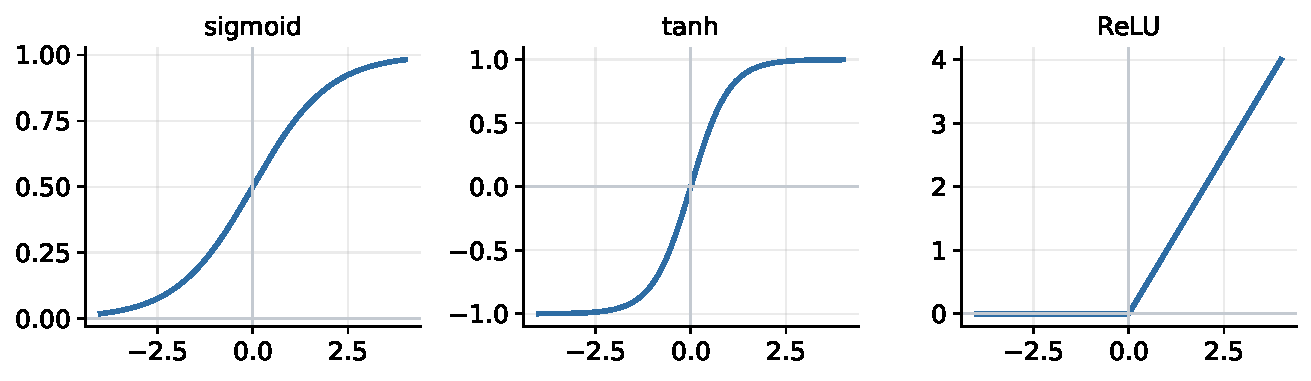
\includegraphics[width=0.78\textwidth]{lecture_6/figures/fig_activations.pdf}
\caption{Activations: the bend between the layers.}
\label{fig:act6}
\end{figure}

At the output, the head and the loss match the task: sigmoid with
log-loss for binary PD (Blocks 2--3's loss, verbatim), softmax with
cross-entropy for the five-class complaint router (Block 5), a linear
unit with squared error for regression. The softmax, for the record, is
$p_k = e^{z_k} / \sum_j e^{z_j}$ - the multi-way sigmoid: five scores
in, five probabilities out, summing to one. The body of the network is
task-agnostic feature machinery; only the head and the loss change -
one body, exchangeable heads, which is the design idea that carries all
of deep learning (and, in passing, is all multi-task learning is).

\subsubsection{Backpropagation: the chain rule doing bookkeeping}
Training is bookkeeping, not magic: forward pass, log-loss, then
\emph{backpropagation} - the chain rule attributing a share of the error
to every weight - and a small gradient-descent step
$w \leftarrow w - \eta\, \partial L / \partial w$ (with learning rate
$\eta$), repeated over epochs. To see that it really is just the chain
rule, work the smallest network that has any depth at all: one input
$x$, one hidden unit, one output, so
\[
z_1 = w_1 x, \qquad h = \sigma(z_1), \qquad z_2 = w_2 h, \qquad
p = \sigma(z_2),
\]
with log-loss $L = -\,y \log p - (1-y)\log(1-p)$. For the output weight,
the chain rule gives the same beautiful cancellation you met in Block 2:
\[
\frac{\partial L}{\partial w_2}
= \frac{\partial L}{\partial z_2}\cdot\frac{\partial z_2}{\partial w_2}
= (p - y)\, h ,
\]
the residual times the input to that weight. For the hidden weight,
simply keep chaining:
\[
\frac{\partial L}{\partial w_1}
= (p - y)\cdot w_2 \cdot \sigma'(z_1) \cdot x .
\]
Read it right to left: the error signal $(p-y)$ is passed backward
through $w_2$, scaled by the local slope $\sigma'(z_1)$, and finally
multiplied by the input $x$ - exactly the pattern ``error times
downstream weight times local slope times local input'' that repeats at
every layer of every network ever trained. Backpropagation is nothing
more than organising this computation so that each intermediate quantity
is computed once and reused instead of re-derived per weight - the
accountant's trick of running subtotals, which is why the honest name
for it is bookkeeping. You can also now see the vanishing gradient in
the formula: every $\sigma'$ factor is at most $1/4$, and deep chains
multiply many of them.

\subsubsection{Stochastic gradient descent, learning rates, and Adam}
In practice the gradient is estimated on mini-batches
(\emph{stochastic} gradient descent; one pass over all batches is an
epoch). Computing the exact gradient would mean touching every one of
21{,}000 customers before taking a single step - accurate, slow, and
pointless at scale; a random batch of, say, 200 customers gives a noisy
but unbiased estimate at a hundredth of the cost. The noise is even a
feature, not just a tolerated flaw: the jitter helps escape poor
valleys of the non-convex landscape - controlled chaos, cousin to the
bootstrap's controlled resampling in Block 3. The learning rate $\eta$
has simple physics: the loss surface near a minimum is a valley, and
the step you take is $\eta$ times the slope. Too large and you leap
across the valley to the opposite wall - and back, and across again -
settling, if at all, visibly higher than the floor. Too small and each
step is a shuffle: the loss creeps down so slowly the run looks dead.
\textbf{Adam}, the default optimiser, deserves one honest
paragraph: it keeps a running average of each weight's recent gradients
(momentum) and of their recent magnitudes, and scales each weight's
step by the ratio - so weights with consistently small gradients get
proportionally larger steps and vice versa, which makes it far less
temperamental about the initial rate. But it is still gradient descent
with a learning rate you own: Adam removes tantrums, not judgement, and
a bad rate still produces a bad run.

\subsubsection{Initialisation and seeds: why the MLP wobbles when trees
do not}
Unlike OLS there is no closed form, and unlike logistic regression the
landscape is not convex - many valleys, so initialisation and seeds
matter: the reproducibility rule, weights edition. The contrast with the
rest of the course is instructive: a single tree is deterministic given
the data, and a forest averages away its own randomness, but the MLP
starts from \emph{random} initial weights (it must - if all weights
started equal, every unit in a layer would compute the same thing and
receive the same gradient forever; symmetry has to be broken), and
gradient descent then rolls downhill into whichever valley is nearest.
Different seed, different valley, different network, slightly different
AUC. So fix the seed for reproducibility, but never mistake a fixed
seed for stability - run twice with different seeds before claiming an
improvement, and if the seed wobble is bigger than your claimed gain,
you have claimed noise (Block 3's CV-spread discipline, verbatim).

\begin{figure}[htbp]
\centering
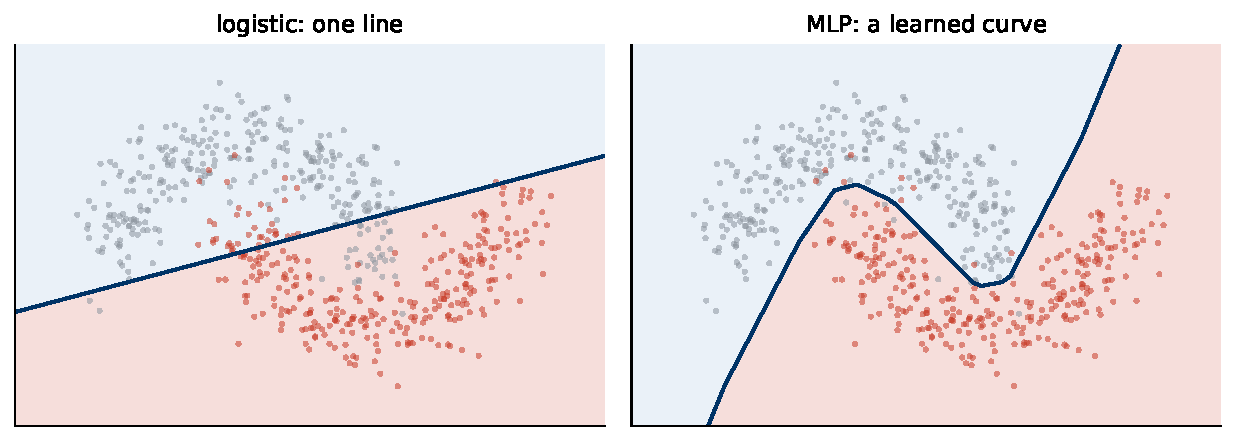
\includegraphics[width=0.78\textwidth]{lecture_6/figures/fig_mlp_boundary.pdf}
\caption{Block 3's crescents, revisited: the MLP learns the curve.}
\label{fig:moons6}
\end{figure}

\begin{figure}[htbp]
\centering
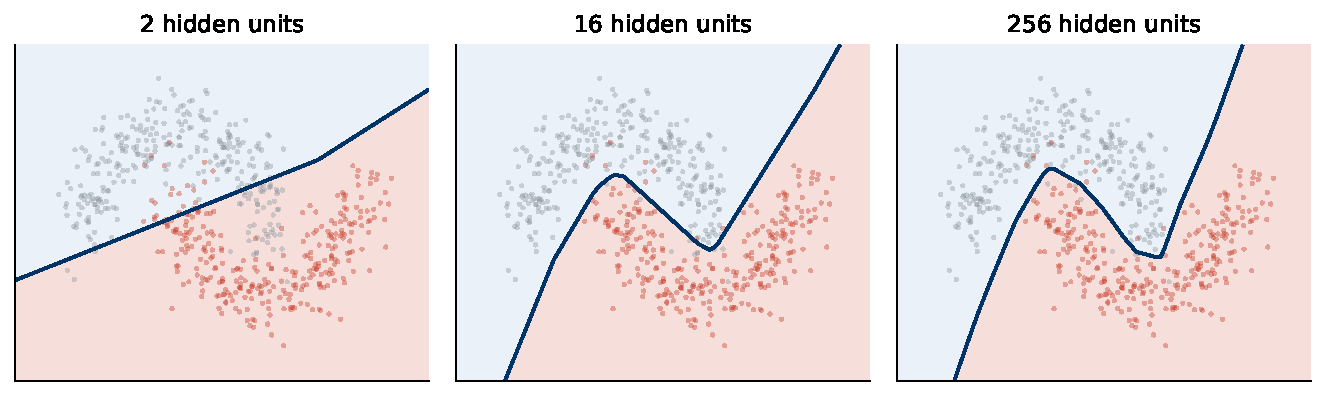
\includegraphics[width=0.82\textwidth]{lecture_6/figures/fig_capacity.pdf}
\caption{Capacity: width is a dial on the same U-curve.}
\label{fig:cap6}
\end{figure}

What the bend buys is visible on the course's favourite crescents
(Figure~\ref{fig:moons6}): logistic must draw a line, the MLP learns a
smooth curve with no hand-engineered features - compare the tree's
staircase from Block 3. And what capacity costs is equally visible
(Figure~\ref{fig:cap6}): two hidden units underfit, 256 memorise the
noise along the edge - the U-curve of Blocks 2 and 3, neural edition,
with width and depth as the capacity dials where degree, depth and
$1/\alpha$ used to be. Universal-approximation folklore (``one
wide-enough layer can fit anything'') is a statement about \emph{can},
not \emph{will}; nothing about neural networks repeals the U-curve.

\subsection{Training realities}

\subsubsection{Reading the canonical plot}
Reading a training run is a skill worth more than any architecture
trivia. The canonical plot (Figure~\ref{fig:loss6}): training loss falls
forever; validation accuracy rises, peaks, and decays as memorisation
sets in - \textbf{early stopping} halts at the peak and is the network's
everyday leash. The shape is inevitable, not accidental: early in
training the network learns genuinely general structure, which also
lives in the validation set, so both curves improve together; past some
point the cheapest way to keep lowering the \emph{training} loss is to
encode the training set's idiosyncrasies - noise, one-off customers,
label quirks - which by definition do not live in the validation set,
so the validation curve turns. The divergence of the two curves is
overfitting watched in real time: the U-curve traced along the
training-time axis instead of the capacity axis.

\subsubsection{Early stopping as regularisation}
That reframing explains why early stopping is a genuine regulariser and
not a mere convenience. Stopping at epoch 40 instead of 400 means the
weights never travelled far from their small random initial values - and
a network whose weights are constrained to stay small is, in effect, a
lower-capacity network - training time functions as a capacity dial.
Halting early is therefore first cousin to weight decay
(which pulls weights toward zero explicitly, ridge-style) and to simply
building a smaller network - three roads to the same place on the
U-curve. The complete leash inventory maps one-to-one onto the course:
early stopping (GBDT's number of rounds), weight decay (ridge), dropout
(randomly silencing units during training, a bagging-flavoured
randomiser), smaller networks (tree depth) - and more data, the only
leash that adds signal rather than restricting the fit. Every mechanism
is new; no idea is new. Ask the fixed question - where is the leash? -
and any future architecture becomes familiar in an afternoon.

\subsubsection{The learning rate, and the practicalities that bite}
The learning rate is the one knob that can consume an evening
(Figure~\ref{fig:lr6}): too high and the steps overshoot the narrow
valley and settle at a visibly worse loss; too low and the network
sleeps; the usable band spans orders of magnitude, so it is searched on
a log scale - try $10^{-1}, 10^{-2}, 10^{-3}, 10^{-4}$ before refining
(Block 3's tuning advice applies verbatim). GBDT's learning rate is the
same concept - humble steps, more of them. Practicalities that bite: scale the features - gradient
descent on unscaled inputs limps, because a feature measured in
thousands drags gradients around while a 0--1 flag whispers, so the
pipeline with a scaler is mandatory again (gradient country, not tree
country); impute-plus-indicator returns, because the MLP has no native
missing-value handling (GBDT stays the more convenient family here);
and everything costs more - minutes-not-milliseconds training, a larger
tuning surface, a hungrier data appetite - all of which must be paid for
by measured accuracy.

\begin{figure}[htbp]
\centering
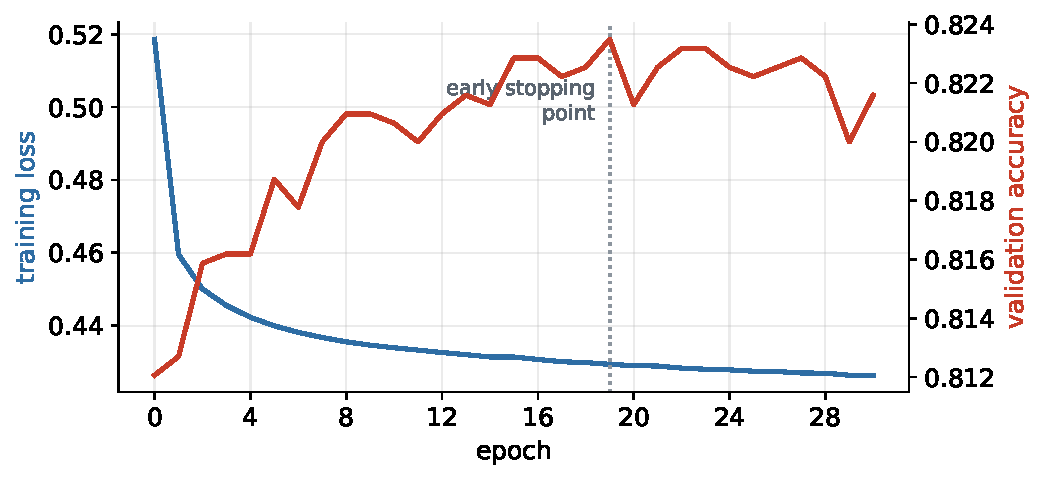
\includegraphics[width=0.6\textwidth]{lecture_6/figures/fig_loss_curve.pdf}
\caption{The canonical training plot, with the early-stopping point.}
\label{fig:loss6}
\end{figure}

\begin{figure}[htbp]
\centering
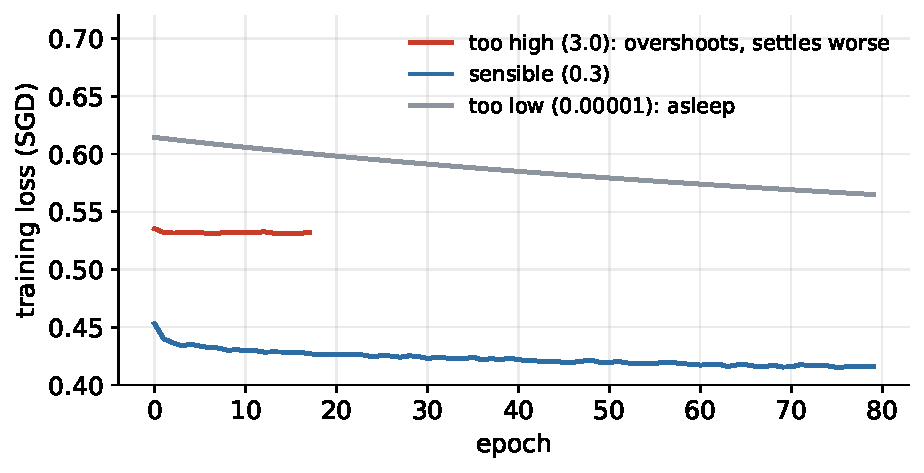
\includegraphics[width=0.6\textwidth]{lecture_6/figures/fig_lr_effect.pdf}
\caption{Three learning rates: overshoot, sensible, asleep.}
\label{fig:lr6}
\end{figure}

\subsubsection{Debugging a training run: the field checklist, in prose}
A field checklist for broken runs, expanded into the reasoning behind
each line. \emph{Loss is NaN or exploding}: the learning rate is too
high - each overshoot lands on a steeper slope, the next step is larger
still, and within a few iterations the weights overflow; drop the rate
tenfold and restart. \emph{Loss flat from epoch one}: three suspects,
checked in order - the rate is too low, the features are unscaled (one
loud feature dominating every gradient), or a layer of ReLUs has died
(all units stuck negative, passing zero gradient - often the scar of an
earlier too-high rate). \emph{Train great, validation ugly}: the
U-curve says hello - tighten a leash. And the classic smoke test: a
healthy network memorises 100 rows perfectly - 897 parameters should
crush 100 points - so if yours cannot, the bug is in the pipeline (a
label misaligned with its features, a broken scaler, a wrong loss), not
in your patience. Note the shape of this list: it is Block 1's
read-the-traceback discipline, upgraded to a stochastic system where
the failure is a curve, not an exception.

\begin{practice}
sklearn's \texttt{MLPClassifier} inside a pipeline is enough for
foundations and for this course's tournament; industry reaches for
PyTorch when architectures get custom. The habits transfer unchanged.
\end{practice}

\subsection{The verdict}
The final tournament (Figure~\ref{fig:final6}) closes the course's
longest-running experiment: MLP 0.759 - clearing the baseline (0.731) by
almost three points, so complexity earned its keep - yet still behind
the tuned GBDT (0.773). The real portfolio's final order reads GBDT $>$
MLP $>$ SVM $\approx$ logistic (the Block 3 interlude's SVM entered the
same tournament at 0.715): the most fashionable family takes second
place, and the tabular crown stays with boosted trees, exactly as the
benchmark literature predicts.

\begin{figure}[htbp]
\centering
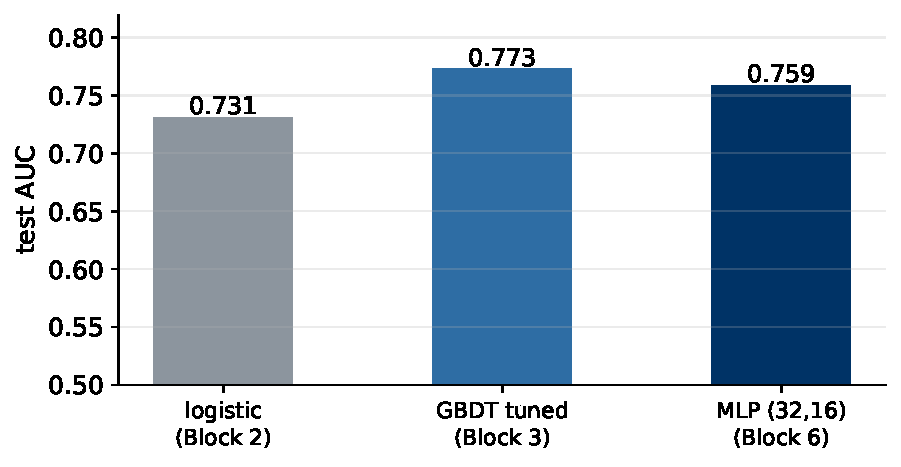
\includegraphics[width=0.56\textwidth]{lecture_6/figures/fig_final_tournament.pdf}
\caption{The final tournament: the crown stays with boosted trees.}
\label{fig:final6}
\end{figure}

\subsubsection{Where neural networks actually win}
That benchmark literature deserves an honest summary, because our
result is one instance of it. Across repeated public comparisons on
mid-size tabular problems - tens of columns, thousands to hundreds of
thousands of rows, the shape of most credit, churn and pricing datasets
- tuned gradient-boosted trees win most of the time, deep models win
sometimes, and the margin either way is usually modest. The structural
reason: tabular columns are heterogeneous and individually meaningful,
with no spatial or sequential arrangement for layers to exploit, so the
MLP spends capacity rediscovering what column structure gives trees for
free. Our 0.759 versus 0.773 is that paragraph in one line. Neural
networks win elsewhere, and win by
knockout: perception and sequence data - images, speech, text, time
series - where layers exploit structure that tabular rows lack (pixels
near pixels, words after words), and where the network's real product is
\emph{representation learning}: the hidden layers learn the features
that decades of hand-crafted pipelines failed to. Genuine tabular wins
exist too: entity embeddings for thousand-category features such as
merchant IDs, learned into dense vectors - the same idea as Block 5's
word embeddings; and representation reuse - autoencoders (Block 4's
reconstruction lens gone nonlinear, useful for anomaly scores) and
pretrained models. The shop rule, final form: logistic $\to$ GBDT $\to$
deep, each step only after the previous one is beaten on honest
numbers. What the course skipped on purpose - CNNs, transformers and
attention, pretraining - each reduces to one focused week of reading
once the neuron, the loss, SGD and the leash inventory are owned.

\subsubsection{The interpretability bill}
The interpretability bill prices the trade: Block 2's receipt was exact
and free - every coefficient a signed, quantified statement you could
read to a customer - and the tree's path was at least readable; the
MLP's hundreds of weights carry no individual meaning, so explanation
becomes approximate reconstruction (SHAP and friends): fitting an
explanatory account \emph{around} the model rather than reading one
\emph{off} it. Two practical shapes of that reconstruction: reason codes
- the top features pushing this customer's score toward decline,
extracted per decision and required, in some form, wherever adverse
decisions must be explained - and global surrogates, a small tree or
linear model trained to mimic the network, faithful in bulk but never
guaranteed faithful for the one customer on the phone. In regulated
lending the bill is concrete: adverse-action reasons that must be true,
model-validation teams that must reproduce and attack the model, and
regulator Q\&A - each harder, slower, more contestable than with the
receipt. The trade is therefore not accuracy versus beauty but accuracy
versus auditability, monitoring cost and legal risk - priced per use
case: a half-point of AUC that costs your explanation is a bad trade at
a bank and a fine one in ad ranking. Context prices it.

\subsection{Responsible ML}
A wrong sales forecast wastes money; a wrong credit model declines the
wrong people, systematically, at scale, silently - the social
consequences the course outcomes name as K3. Every earlier block planted
a piece - selection bias (Block 1), probabilities that price people
(Blocks 2--3), segments that must not decide (Block 4), PII in text
(Block 5) - and this section assembles them on our own model's numbers,
not hypotheticals. The operating question is never ``is the model
accurate?''; it is ``what does the model do to people, and who
checked?''

\subsubsection{The legal floor}
The legal floor (EU, sketched; the real thing is done with lawyers in
the room) has four planks. First, \textbf{GDPR Article~22}: a person
has the right not to be subject to a decision based \emph{solely} on
automated processing when it produces legal effects or similarly
significantly affects them - and credit refusal is the textbook case.
Automated decisions are permitted under exceptions (contractual
necessity among them), but only with safeguards: the right to obtain
human intervention, to express one's point of view, and to contest;
alongside it, the GDPR's transparency articles require \emph{meaningful
information about the logic involved} - not the weights file, but a
truthful, comprehensible account of what drives the decision. Second,
the \textbf{duty to state reasons}: declined customers are informed of
the grounds, and the grounds must be true ones - Block 1's punchline
about truthful reasons was never merely imputation hygiene; the US
calls this ``adverse action.'' Third, \textbf{protected attributes}:
sex, ethnicity and friends are off-limits for credit decisions - which
is precisely why the audit below runs by sex - with age in a grey,
jurisdiction-dependent zone (hence a lab exercise, not a lecture
assertion). Fourth, the \textbf{EU AI Act} lists creditworthiness
assessment as high-risk, which converts a familiar list from best
practice into statute: risk management, data governance, technical
documentation and logging, transparency, human oversight, demonstrated
accuracy and robustness. Your job as a builder is not to practise law;
it is to know when to invite the lawyers - earlier than feels natural.

\subsubsection{Where bias enters: the doors}
Bias needs no malice to enter - it has doors, and each door is a
mechanism you can name. \emph{Labels}: ``default'' is not a fact of
nature but a record of past collection practices - if one group was
historically pursued harder, its recorded default rate is inflated, and
the model faithfully learns the inflation (historical bias, living in
the target). \emph{Selection}: the training data contains approved
customers only; the rejected are absent by construction (Block 1), so
the model learns the approved world and is deployed on the whole one.
\emph{Features}: proxies encode group membership without naming it -
more below. \emph{Measurement}: the same quantity is captured with
different fidelity across segments - income verified for some and
self-declared for others is two different features wearing one column
name. \emph{Objective}: optimising average
cost ignores who pays it; a threshold that is cost-optimal in aggregate
can concentrate its errors in one group. And \emph{feedback loops} -
selection bias motorised. Walk the credit example through one full turn:
the model declines a group at a higher rate; fewer loans to that group
are observed; there is consequently no evidence the declines were wrong
(a declined customer generates no repayment record); next year's model,
trained on the new data, declines them again - now with better
``justification.'' The model does not merely inherit the bias; it
manufactures more of it, and every system that acts on its own
predictions contains such a loop somewhere. Loop breakers: reject
inference (Block 1's vocabulary), deliberate exploration - approve a
small random slice near the boundary, expensive but informative - and
monitoring group gaps over vintages, not snapshots. None of these doors
is opened by malice. All of them are opened by default, unless someone
checks.

\subsubsection{Fairness, formally - and why you must choose}
Fairness itself has competing formalisations. For a protected group $g$,
decision $\hat{y}$ (1 = decline) and outcome $y$ (1 = default):
\emph{demographic parity} demands equal decline rates,
$P(\hat{y}{=}1 \mid g)$ equal across groups; \emph{equalised odds}
demands equal error rates - the same FPR (creditworthy people wrongly
declined) and FNR (defaulters missed) in every group; \emph{calibration
within groups} demands that a predicted 0.3 means 0.3 for everyone -
$P(y{=}1 \mid \hat{p}, g)$ independent of $g$. All three sound obviously
right, and the impossibility results of Kleinberg et al.\ and
Chouldechova say they cannot all hold at once when base rates differ.
A toy portfolio makes the conflict tangible. Two groups of 100
applicants; group A contains 30 true future defaulters, group B contains
10 - differing base rates, as in every real portfolio. Give yourself the
best possible model: a perfect one, declining exactly the future
defaulters. It satisfies equalised odds trivially (FPR and FNR are zero
in both groups) and is perfectly calibrated - yet it declines 30\% of
group A and 10\% of group B, violating demographic parity by 20 points.
Now force parity instead, say by declining 20\% of each group: in group
A you must approve 10 future defaulters (misses), and in group B you
must decline 10 creditworthy people (false positives) - you have
manufactured unequal error rates to equalise decline rates. The general
lesson is exactly this arithmetic: when base rates differ, decline
rates, error rates and calibration are linked by accounting identities,
and equalising one forces gaps in another. ``Make it fair'' is therefore
not a specification; \emph{choosing which fairness} is the decision,
and it is not the data scientist's alone.

\begin{figure}[htbp]
\centering
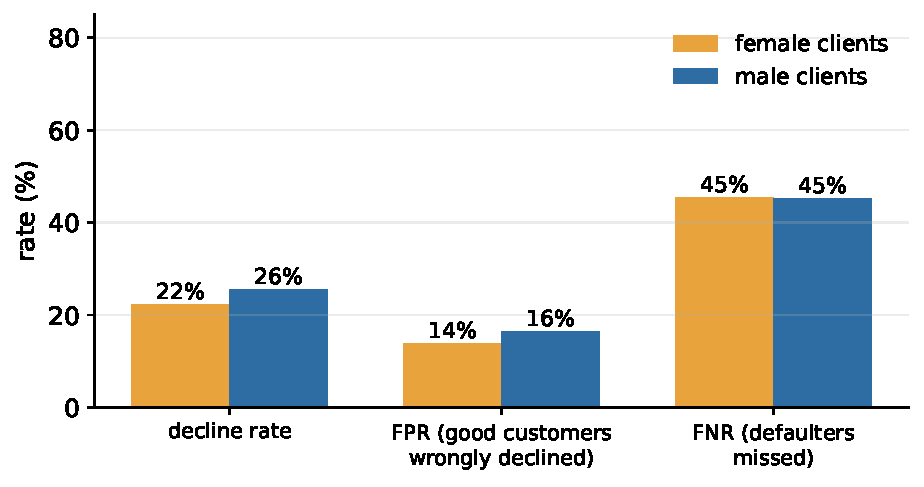
\includegraphics[width=0.66\textwidth]{lecture_6/figures/fig_fairness.pdf}
\caption{Our own model, audited by sex at the cost-optimal threshold.}
\label{fig:fair6}
\end{figure}

\begin{figure}[htbp]
\centering
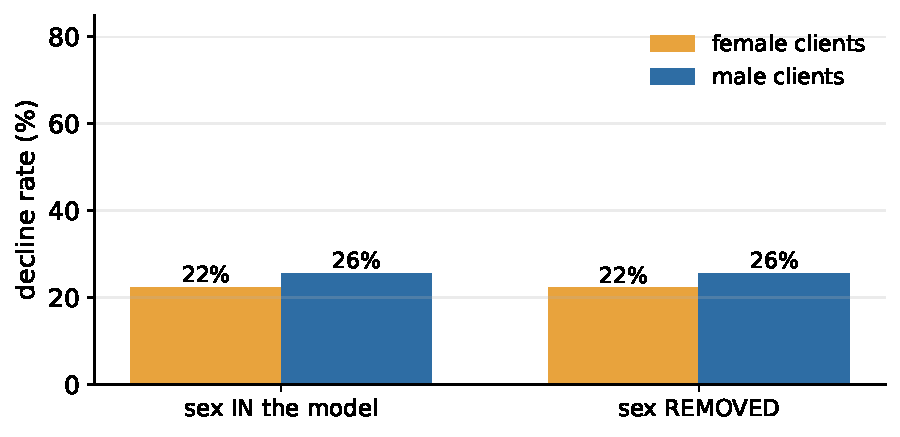
\includegraphics[width=0.6\textwidth]{lecture_6/figures/fig_proxy.pdf}
\caption{The unawareness experiment: removing sex changes essentially
nothing - the behaviour already carries the information.}
\label{fig:proxy6}
\end{figure}

\subsubsection{The audit, on real people}
Then the audit itself, on real people: our GBDT at Block 3's
cost-optimal threshold (0.26), split by sex - an unambiguously protected
attribute (Figure~\ref{fig:fair6}). Men are declined at 25.6\% versus
22.3\% for women, wrongly declined (FPR) at 16.5\% versus 13.8\% - with
base default rates of 23.9\% versus 21.0\%. Read honestly: the gaps are
modest and track the base-rate difference - the 3.3-point decline gap
sits close to the 2.9-point base-rate gap - so this model does not
amplify what the portfolio brought in. The verdict could have gone the
other way: on the synthetic portfolio an age audit once turned a
3.6-point base gap into an 18-point decline gap - a model that
manufactures disparity far beyond what the data contains - and nothing
about the two models' code or AUC would have told you which one you
had. The only way to know which model you have is to measure.

\subsubsection{Proxy discrimination: why removal fails}
The ``just remove sex'' experiment (Figure~\ref{fig:proxy6}) then lands
the proxy lesson in its purest form: retrain the identical pipeline
without the column, and removal changes essentially nothing - every bar
identical - because six months of payment behaviour already carries
whatever group structure exists. The model never needed the label: any
feature correlated with group membership lets it reconstruct the group
statistically, without anyone intending it. Deleting the label does not
delete the information; ``fairness through unawareness'' here is free
and toothless at once. The corollary cuts deep: if the measured gaps
had needed fixing, no edit to the column list would have fixed them -
any real repair would have to act on \emph{decisions} (thresholds,
constraints, data), not on feature names. This is why blindness-based
compliance arguments (``the model cannot discriminate, it never sees
sex'') fail on contact with data, and why the audit measures outcomes
rather than inputs.

\subsubsection{Mitigation and governance}
The mitigation menu spans three stages of the pipeline.
\emph{Pre-processing} - fix the data: rebalance, collect better labels,
attack selection bias at its source (recall that the rejected are
missing by construction). \emph{In-processing} - fairness constraints
inside training, such as equalised-odds penalties added to the loss;
Block 3's monotonic constraints were a mild cousin of the same move.
\emph{Post-processing} - per-group thresholds: effective and
transparent in exactly the way the toy arithmetic above suggests, and
legally delicate, because it explicitly uses the protected attribute to
repair its own harm - a decision that belongs with lawyers, not in a
notebook. One option is always available and never delicate: measure
the gaps and publish them internally, so that the people entitled to
decide the trade-off can decide it with numbers in front of them.
Toolkits exist (fairlearn, AIF360); the hard part was never the code.

Responsibility extends past fairness: drift monitoring that watches gaps
and not just Gini - portfolios move, and yesterday's fair model can be
today's unfair one; documentation - time-travel audits, imputation
recipes, threshold rationales, fairness measurements - because at audit
time the written trail \emph{is} the model; human oversight as
architecture, not UX - Block 5's confidence bars and queues, statutory
under the AI Act; and data minimisation - collect what the decision
needs, not what the crawler found. Governance assigns the seats: the
builder is the first line - measurements, documentation, honesty
clauses, everything this course drilled; independent model validation
is the second - a professional adversarial verifier that rebuilds your
results and attacks your assumptions (a common first job for graduates
of courses like this one); the model-risk committee owns the
trade-offs no analyst should carry alone (which fairness, whose cost);
audit and regulator arrive later and read everything. The take-home
checklist has six lines - when is each feature known and may we use it
(two written answers per column); gaps measured (decline, FPR, FNR,
calibration by group) before go-live and on schedule after; a true
explanation path per declined customer; a reachable human who can
overrule; alarms on drift and on gap widening; an owner who is a name,
not a department - and most real-world model-risk findings are a
missing line from it.

\subsection{Defence briefing, exam, and the course in five sentences}
The lab notebook \texttt{06\_neural\_networks} trains the MLP in a
pipeline, reads its loss curve, sweeps the learning rate, reruns the
final tournament, and then performs the fairness audit - the group
report by sex at the cost-optimal threshold, the age audit as an
exercise, and the sex-removal experiment - ending with the exercise that
matters beyond the course: run the same audit on your own project's
model and put the table in your limitations section. ``Done'' means your
MLP verdict matches your tournament table and your fairness audit has
numbers in it.

The defence briefing: presentations run $\sim$6--8 minutes plus
questions - business framing, data work, two model families against a
baseline, honest evaluation, recommendation - with all code and the
exact final slides uploaded before Block 7 starts; notebooks must
survive Restart \& Run All (the habit since Block 1 - this is why); the
honesty kit (CV spread, leakage audit, threshold argument, limitations
paragraph) is the differentiator; and AI assistants were allowed all
semester, but you answer for every submitted line - expect to explain
and modify your code live. The canonical failure modes, from the
graveyard: a proud suspicious AUC (find the leak before we do),
unexamined accuracy on an imbalanced target, complexity without a
baseline, structure without honesty clauses, an order-dependent
notebook, and analysis that ends in metrics instead of a decision. The
exam (term 0, 120 minutes) weighs conceptual multiple choice at
$\sim$40\% and short open questions at $\sim$60\%, testing selection and
interpretation - ``here is a confusion matrix, a rule, a coefficient, a
dendrogram: what do you tell the business?'' - not derivations; the
worked-example slides calibrate the by-hand questions, and the six
``Block $N$ in five sentences'' slides are the compressed syllabus.

The course itself compresses to five: start from the decision; judge on
unseen data with money attached; every family has a leash and complexity
must earn its keep; unlabelled structure is found, argued and named
honestly; and models act on people - explanations, fairness gaps and
human oversight are deliverables, not decoration. The subtitle kept its
promise: how not to fool yourself.

% =====================================================================
\section{Block 7 - Defences \& exam}
Project presentations ($\sim$6--8 minutes per team) in part one; written exam
(term 0) in part two. Details in Appendix~\ref{app:org}.

% =====================================================================
\appendix
% =====================================================================
\section{Course organisation and assessment}
\label{app:org}

\subsection{Course at a glance}
\begin{center}
\begin{tabular}{@{}ll@{}}
\toprule
Programme & SMMD-ADA: Analiza danych -- Big Data (full-time, second cycle); \\
          & English-language equivalent: SMMD-AAB \\
Also elective for & SMMD-EKO (Economics; likewise SMMD-QEM) and SMMD-MIS \\
          & (Quantitative Methods in Economics and Information Systems) \\
Language & English (deliverables in English) \\
Meetings & 7 blocks, Tuesdays 17:10--20:30, Group 120 \\
Dates & 06.10, 13.10, 20.10, 27.10, 03.11, 10.11, 17.11 \\
Assessment & Project 50\% + Exam (term 0) 50\%; pass $\geq$ 60\% overall \\
Prerequisite & Basic Python fluency (see primer notebook \texttt{00}) \\
Running example & Retail-credit / PD (probability-of-default) portfolio \\
Tooling & Python, \texttt{scikit-learn}, \texttt{pandas}; Jupyter / Colab; \texttt{uv} \\
\bottomrule
\end{tabular}
\end{center}

\subsection{Learning outcomes}
On the university description, students should:

\paragraph{Knowledge (W).}
\begin{description}[leftmargin=3.2em,style=nextline,itemsep=1pt]
  \item[W1] Know and understand the steps of data mining from structured and unstructured data.
  \item[W2] Understand data-mining methods and models, and the basics of text-mining theory.
  \item[W3] Be able to select the proper methods/models for a specific decision problem.
  \item[W4] Understand the idea of the presented algorithms and the interpretation of results.
\end{description}

\paragraph{Skills (U).}
\begin{description}[leftmargin=3.2em,style=nextline,itemsep=1pt]
  \item[U1] Solve a decision problem using the proper software.
  \item[U2] Prepare data for a data-mining method.
  \item[U3] Estimate data-mining models.
  \item[U4] Assess the quality of estimated models.
  \item[U5] Understand advantages and disadvantages of applied methods.
\end{description}

\paragraph{Social competences (K).}
\begin{description}[leftmargin=3.2em,style=nextline,itemsep=1pt]
  \item[K1] Appreciate the meaning of data analysis in enterprises.
  \item[K2] Be able to assess the acquired knowledge in practical use.
  \item[K3] Understand the social consequences of a wrong analysis.
\end{description}

\subsection{Outcome $\leftrightarrow$ block coverage matrix}
\begin{center}\small
\begin{tabular}{@{}lccccccc|cc@{}}
\toprule
 & B1 & B2 & B3 & B4 & B5 & B6 & B7 & Proj. & Exam \\
\midrule
W1 & \yes & \yes &      &      & \yes &      &      & \yes & \yes \\
W2 &      & \yes & \yes & \yes & \yes & \yes &      & \yes & \yes \\
W3 &      & \yes & \yes & \yes & \yes & \yes & \yes & \yes & \yes \\
W4 & \yes & \yes & \yes & \yes & \yes & \yes &      & \yes & \yes \\
U1 & \yes & \yes & \yes & \yes & \yes & \yes &      & \yes &      \\
U2 & \yes & \yes & \yes & \yes & \yes &      &      & \yes &      \\
U3 &      & \yes & \yes & \yes & \yes & \yes &      & \yes &      \\
U4 &      & \yes & \yes & \yes &      & \yes &      & \yes & \yes \\
U5 &      & \yes & \yes & \yes & \yes & \yes &      & \yes & \yes \\
K1 & \yes &      &      &      &      &      & \yes & \yes &      \\
K2 &      &      & \yes & \yes & \yes & \yes & \yes & \yes &      \\
K3 & \yes &      & \yes &      &      & \yes &      & \yes & \yes \\
\bottomrule
\end{tabular}
\end{center}

\subsection{Project (50\%)}
\textbf{Format.} Teams of 3. A full mini CRISP-DM cycle on a dataset of the
team's choice: business framing $\rightarrow$ data preparation $\rightarrow$
at least two model families $\rightarrow$ correct evaluation $\rightarrow$
interpretation $\rightarrow$ a recommendation. The project ends with a
presentation of results in Block 7 (the last class).\\
\textbf{Deliverables.} (i) all code, as a reproducible notebook, and (ii) the
exact presentation to be shown - both uploaded \emph{before Block 7 starts}.
The presentation itself runs $\sim$6--8 minutes plus questions.\\
\textbf{Data.} The team's own choice: any real dataset that can carry the
full cycle - a meaningful business decision, a predictable target, and enough
rows for an honest split. Typical sources: Kaggle, the UCI repository, open
government data. The choice is declared in the topic description due before
Block 3, which is also where it is approved; teams unsure whether a dataset
qualifies should ask before the deadline.\\
\textbf{Deadlines.} Teams of 3: before Block 2 (13.10). Topic plus a short
written description (the decision, the dataset, the target, the planned two
model families): before Block 3 (20.10) - students without an idea should
consult before the deadline. Code and presentation: uploaded before Block 7
(17.11).\\
\textbf{A sensible week-by-week split.} Week 1: form the team; first contact
with a candidate dataset (\texttt{head}/\texttt{info}/\texttt{describe},
target balance, a missingness map). Week 2: topic and description; EDA of the
chosen data - distributions, bivariate plots against the target, data-quality
risks. Week 3: data preparation (imputation with indicators, one-hot
encoding) and the baseline - logistic regression in a scaled pipeline (or
linear regression for a numeric target) on a stratified, seeded split, plus a
written leakage audit. Week 4: the second family (random forest or gradient
boosting) and the evaluation kit - CV mean $\pm$ sd, ROC/PR, calibration, a
cost-based threshold. Week 5: an optional add-on (segmentation, rules, or
text features) only if it serves the business question; interpretation and a
written recommendation; the presentation skeleton. Week 6: freeze the
notebook (Restart \& Run All), finish the slides, rehearse, and upload.\\
\textbf{Use of AI.} Assistants are allowed, but each student answers for every
submitted line. Every submission is read for the fingerprints of unchecked
generation: conventions nobody in the team can explain, claims that do not
match what the notebook actually computes, boilerplate that ignores the
course's methods. The stronger the impression that the project was produced
solely by AI, the harder the questions at the defence - students should expect
to explain, justify, and modify any part of their code live. Work a team
cannot explain is treated as work the team did not do.

\subsubsection{Rubric (mapped to outcomes)}
\begin{center}\small
\begin{tabular}{@{}p{6.8cm}cl@{}}
\toprule
Criterion & Weight & Outcomes \\
\midrule
Business framing \& problem definition & 10\% & W3, K1 \\
Data preparation \& missingness handling & 15\% & U2, W1 \\
Modelling: $\geq$2 families, justified & 15\% & W2--W3, U3 \\
Evaluation: correct, leakage-aware & 20\% & U4, W4 \\
Interpretation \& recommendation & 15\% & U5, K2 \\
Reproducibility & 5\% & U1 \\
Presentation \& defence & 20\% & K2, K3 \\
\bottomrule
\end{tabular}
\end{center}

\subsection{Exam - term 0 (50\%)}
Held in the second part of Block 7.
\begin{itemize}[leftmargin=1.4em,itemsep=1pt]
  \item $\sim$40\% conceptual multiple choice (definitions, when-to-use, reading a metric).
  \item $\sim$60\% short open questions: pick a method for a described problem and
        interpret a given result.
\end{itemize}
\textbf{Passing.} Project and exam are weighted 50/50; a student passes with
$\geq 60\%$ of the combined score.

\subsection{Datasets \& tooling}
\begin{description}[leftmargin=1.4em,style=nextline,itemsep=2pt]
  \item[Running example: retail-credit / PD portfolio.] Loaded via the shared
        \texttt{finance\_data.load\_credit()} helper, which fetches the German
        Credit (Statlog) set from OpenML and falls back to a realistic synthetic
        Polish credit portfolio when offline. Carries built-in missingness of
        every type and one deliberate leakage column.
  \item[Block 5 add-ons.] Product cross-holding baskets (Market Basket) and a
        consumer-complaint text corpus for text mining.
  \item[Environment.] Python 3, \texttt{scikit-learn}, \texttt{pandas},
        \texttt{matplotlib}, \texttt{mlxtend}; \texttt{uv sync} in the course
        repository creates the environment; runs locally or on Google Colab.
        Non-programmers start with notebook \texttt{00\_python\_primer}.
  \item[Further reading.] James, Witten, Hastie \& Tibshirani, \emph{An
        Introduction to Statistical Learning} (free PDF); Géron,
        \emph{Hands-On Machine Learning}; the scikit-learn User Guide; Kaggle
        write-ups, read critically.
\end{description}

\end{document}
